\documentclass[spanish]{beamer}

%%% CODIFICACIÓN

\usepackage[utf8]{inputenc}
\usepackage[spanish]{babel}
\usepackage{graphics,tikz}

%%% FUENTES

\usepackage[T1]{fontenc}
\usepackage[familydefault,regular]{Chivo}
\usepackage{newtxsf} % Fuente de matemáticas

\setbeamertemplate{navigation symbols}{}

%%% COLORES

\definecolor{background}{RGB}{237,237,237}
\definecolor{text}{RGB}{78,78,78}
\definecolor{accent}{RGB}{129, 26, 24}

\setbeamerfont{framesubtitle}{size=\normalfont\tiny}
\setbeamercolor{framesubtitle}{fg=white}


%%% AJUSTES DE BEAMER

% ¿Negrita en el título de diapositiva o no?
%\setbeamertemplate{frametitle}{\color{accent}\vspace*{1cm}\bfseries\insertframetitle\par\vskip-6pt}

\setbeamertemplate{frametitle}{\color{accent}\vspace*{1cm}\insertframetitle\par\vskip-6pt}

\setbeamertemplate{itemize items}[circle] % Viñetas de itemize

%%% CONFIGURACIÓN DE COLORES DE BEAMER

\setbeamercolor{background canvas}{bg=background}
\setbeamercolor{normal text}{fg=text}
\setbeamercolor{alerted text}{fg=accent}
\setbeamercolor{block title}{fg=accent}
\setbeamercolor{alerted text}{fg=accent}
\setbeamercolor{itemize item}{fg=accent}
\setbeamercolor{enumerate item}{fg=accent}
\setbeamercolor*{title}{fg=accent}
\setbeamercolor{qed symbol}{fg=accent}
\usebeamercolor[fg]{normal text}

%%% PGFPLOTSTABLE

\usepackage{pgfplotstable}


\pgfplotstableset{
columns/0/.style={
     column name={Elementos},
   },
columns/1/.style={
     column name={Tiempo en segundos},
   },
}

%%% INFORMACIÓN DEL DOCUMENTO

\title{Algorítmica: práctica 1}
\subtitle{Análisis de la eficiencia de algoritmos}
\author{Sofía Almeida Bruno\\ Antonio Coín Castro\\ María Victoria Granados Pozo\\ Miguel Lentisco Ballesteros\\ José María Martín Luque\\ \vspace{1em}Grupo 2}
\begin{document}




\maketitle

\begin{frame}{Objetivo}
	Estudiar la eficiencia teórica, empírica e híbrida de 8 algoritmos. También, realizar comparaciones entre sus tiempos de ejecución, así como la influencia de otros factores, como S.O. utilizado o prestaciones del PC.
	
	\begin{itemize}
		\item Burbuja, Inserción y Selección
		\item Mergesort, Quicksort y Heapsort
		\item Floyd
		\item Hanoi
	\end{itemize}
\end{frame}

\begin{frame}{Burbuja}
	Revisa cada elemento de la lista con el siguiente, intercambiándose de posición si no están en el orden correcto.
	
	\vskip 0.5cm
	
	Es $O(n^2)$.
	
\end{frame}

\begin{frame}{}
	\begin{center}
		% GNUPLOT: LaTeX picture with Postscript
\begingroup
  \makeatletter
  \providecommand\color[2][]{%
    \GenericError{(gnuplot) \space\space\space\@spaces}{%
      Package color not loaded in conjunction with
      terminal option `colourtext'%
    }{See the gnuplot documentation for explanation.%
    }{Either use 'blacktext' in gnuplot or load the package
      color.sty in LaTeX.}%
    \renewcommand\color[2][]{}%
  }%
  \providecommand\includegraphics[2][]{%
    \GenericError{(gnuplot) \space\space\space\@spaces}{%
      Package graphicx or graphics not loaded%
    }{See the gnuplot documentation for explanation.%
    }{The gnuplot epslatex terminal needs graphicx.sty or graphics.sty.}%
    \renewcommand\includegraphics[2][]{}%
  }%
  \providecommand\rotatebox[2]{#2}%
  \@ifundefined{ifGPcolor}{%
    \newif\ifGPcolor
    \GPcolortrue
  }{}%
  \@ifundefined{ifGPblacktext}{%
    \newif\ifGPblacktext
    \GPblacktextfalse
  }{}%
  % define a \g@addto@macro without @ in the name:
  \let\gplgaddtomacro\g@addto@macro
  % define empty templates for all commands taking text:
  \gdef\gplbacktext{}%
  \gdef\gplfronttext{}%
  \makeatother
  \ifGPblacktext
    % no textcolor at all
    \def\colorrgb#1{}%
    \def\colorgray#1{}%
  \else
    % gray or color?
    \ifGPcolor
      \def\colorrgb#1{\color[rgb]{#1}}%
      \def\colorgray#1{\color[gray]{#1}}%
      \expandafter\def\csname LTw\endcsname{\color{white}}%
      \expandafter\def\csname LTb\endcsname{\color{black}}%
      \expandafter\def\csname LTa\endcsname{\color{black}}%
      \expandafter\def\csname LT0\endcsname{\color[rgb]{1,0,0}}%
      \expandafter\def\csname LT1\endcsname{\color[rgb]{0,1,0}}%
      \expandafter\def\csname LT2\endcsname{\color[rgb]{0,0,1}}%
      \expandafter\def\csname LT3\endcsname{\color[rgb]{1,0,1}}%
      \expandafter\def\csname LT4\endcsname{\color[rgb]{0,1,1}}%
      \expandafter\def\csname LT5\endcsname{\color[rgb]{1,1,0}}%
      \expandafter\def\csname LT6\endcsname{\color[rgb]{0,0,0}}%
      \expandafter\def\csname LT7\endcsname{\color[rgb]{1,0.3,0}}%
      \expandafter\def\csname LT8\endcsname{\color[rgb]{0.5,0.5,0.5}}%
    \else
      % gray
      \def\colorrgb#1{\color{black}}%
      \def\colorgray#1{\color[gray]{#1}}%
      \expandafter\def\csname LTw\endcsname{\color{white}}%
      \expandafter\def\csname LTb\endcsname{\color{black}}%
      \expandafter\def\csname LTa\endcsname{\color{black}}%
      \expandafter\def\csname LT0\endcsname{\color{black}}%
      \expandafter\def\csname LT1\endcsname{\color{black}}%
      \expandafter\def\csname LT2\endcsname{\color{black}}%
      \expandafter\def\csname LT3\endcsname{\color{black}}%
      \expandafter\def\csname LT4\endcsname{\color{black}}%
      \expandafter\def\csname LT5\endcsname{\color{black}}%
      \expandafter\def\csname LT6\endcsname{\color{black}}%
      \expandafter\def\csname LT7\endcsname{\color{black}}%
      \expandafter\def\csname LT8\endcsname{\color{black}}%
    \fi
  \fi
    \setlength{\unitlength}{0.0500bp}%
    \ifx\gptboxheight\undefined%
      \newlength{\gptboxheight}%
      \newlength{\gptboxwidth}%
      \newsavebox{\gptboxtext}%
    \fi%
    \setlength{\fboxrule}{0.5pt}%
    \setlength{\fboxsep}{1pt}%
\begin{picture}(5760.00,4320.00)%
    \gplgaddtomacro\gplbacktext{%
      \colorrgb{0.30,0.30,0.30}%
      \put(990,1153){\makebox(0,0)[r]{\strut{}$\textcolor{text}{0}$}}%
      \colorrgb{0.30,0.30,0.30}%
      \put(990,1466){\makebox(0,0)[r]{\strut{}$\textcolor{text}{1}$}}%
      \colorrgb{0.30,0.30,0.30}%
      \put(990,1780){\makebox(0,0)[r]{\strut{}$\textcolor{text}{2}$}}%
      \colorrgb{0.30,0.30,0.30}%
      \put(990,2093){\makebox(0,0)[r]{\strut{}$\textcolor{text}{3}$}}%
      \colorrgb{0.30,0.30,0.30}%
      \put(990,2406){\makebox(0,0)[r]{\strut{}$\textcolor{text}{4}$}}%
      \colorrgb{0.30,0.30,0.30}%
      \put(990,2719){\makebox(0,0)[r]{\strut{}$\textcolor{text}{5}$}}%
      \colorrgb{0.30,0.30,0.30}%
      \put(990,3033){\makebox(0,0)[r]{\strut{}$\textcolor{text}{6}$}}%
      \colorrgb{0.30,0.30,0.30}%
      \put(990,3346){\makebox(0,0)[r]{\strut{}$\textcolor{text}{7}$}}%
      \colorrgb{0.30,0.30,0.30}%
      \put(990,3659){\makebox(0,0)[r]{\strut{}$\textcolor{text}{8}$}}%
      \colorrgb{0.30,0.30,0.30}%
      \put(1122,1021){\rotatebox{45}{\makebox(0,0)[r]{\strut{}$\textcolor{text}{0}$}}}%
      \colorrgb{0.30,0.30,0.30}%
      \put(1546,1021){\rotatebox{45}{\makebox(0,0)[r]{\strut{}$\textcolor{text}{5000}$}}}%
      \colorrgb{0.30,0.30,0.30}%
      \put(1970,1021){\rotatebox{45}{\makebox(0,0)[r]{\strut{}$\textcolor{text}{10000}$}}}%
      \colorrgb{0.30,0.30,0.30}%
      \put(2394,1021){\rotatebox{45}{\makebox(0,0)[r]{\strut{}$\textcolor{text}{15000}$}}}%
      \colorrgb{0.30,0.30,0.30}%
      \put(2818,1021){\rotatebox{45}{\makebox(0,0)[r]{\strut{}$\textcolor{text}{20000}$}}}%
      \colorrgb{0.30,0.30,0.30}%
      \put(3243,1021){\rotatebox{45}{\makebox(0,0)[r]{\strut{}$\textcolor{text}{25000}$}}}%
      \colorrgb{0.30,0.30,0.30}%
      \put(3667,1021){\rotatebox{45}{\makebox(0,0)[r]{\strut{}$\textcolor{text}{30000}$}}}%
      \colorrgb{0.30,0.30,0.30}%
      \put(4091,1021){\rotatebox{45}{\makebox(0,0)[r]{\strut{}$\textcolor{text}{35000}$}}}%
      \colorrgb{0.30,0.30,0.30}%
      \put(4515,1021){\rotatebox{45}{\makebox(0,0)[r]{\strut{}$\textcolor{text}{40000}$}}}%
      \colorrgb{0.30,0.30,0.30}%
      \put(4939,1021){\rotatebox{45}{\makebox(0,0)[r]{\strut{}$\textcolor{text}{45000}$}}}%
      \colorrgb{0.30,0.30,0.30}%
      \put(5363,1021){\rotatebox{45}{\makebox(0,0)[r]{\strut{}$\textcolor{text}{50000}$}}}%
    }%
    \gplgaddtomacro\gplfronttext{%
      \colorrgb{0.30,0.30,0.30}%
      \put(220,2406){\rotatebox{-270}{\makebox(0,0){\strut{}Tiempo de ejecución (s)}}}%
      \colorrgb{0.30,0.30,0.30}%
      \put(3242,220){\makebox(0,0){\strut{}Tamaño del vector (elementos)}}%
      \colorrgb{0.30,0.30,0.30}%
      \put(3242,3989){\makebox(0,0){\strut{}Eficiencia empírica burbuja-linux-O0}}%
    }%
    \gplbacktext
    \put(0,0){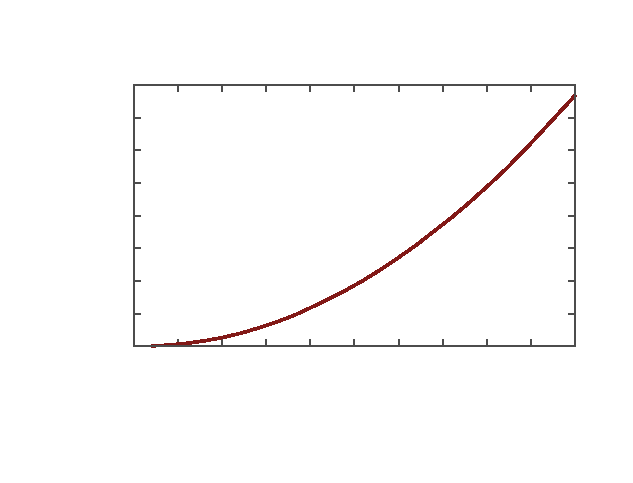
\includegraphics{./graficos/burbuja-linux-O0}}%
    \gplfronttext
  \end{picture}%
\endgroup

	\end{center}
\end{frame}

\begin{frame}{Inserción}
	Consideramos el elemento N-ésimo de la lista y lo ordenamos respecto de los elementos desde el primero hasta el N-1-ésimo.
	
	\vskip 0.5cm
	
	Es $O(n^2)$.
\end{frame}

\begin{frame}
	\begin{center}
		% GNUPLOT: LaTeX picture with Postscript
\begingroup
  \makeatletter
  \providecommand\color[2][]{%
    \GenericError{(gnuplot) \space\space\space\@spaces}{%
      Package color not loaded in conjunction with
      terminal option `colourtext'%
    }{See the gnuplot documentation for explanation.%
    }{Either use 'blacktext' in gnuplot or load the package
      color.sty in LaTeX.}%
    \renewcommand\color[2][]{}%
  }%
  \providecommand\includegraphics[2][]{%
    \GenericError{(gnuplot) \space\space\space\@spaces}{%
      Package graphicx or graphics not loaded%
    }{See the gnuplot documentation for explanation.%
    }{The gnuplot epslatex terminal needs graphicx.sty or graphics.sty.}%
    \renewcommand\includegraphics[2][]{}%
  }%
  \providecommand\rotatebox[2]{#2}%
  \@ifundefined{ifGPcolor}{%
    \newif\ifGPcolor
    \GPcolortrue
  }{}%
  \@ifundefined{ifGPblacktext}{%
    \newif\ifGPblacktext
    \GPblacktextfalse
  }{}%
  % define a \g@addto@macro without @ in the name:
  \let\gplgaddtomacro\g@addto@macro
  % define empty templates for all commands taking text:
  \gdef\gplbacktext{}%
  \gdef\gplfronttext{}%
  \makeatother
  \ifGPblacktext
    % no textcolor at all
    \def\colorrgb#1{}%
    \def\colorgray#1{}%
  \else
    % gray or color?
    \ifGPcolor
      \def\colorrgb#1{\color[rgb]{#1}}%
      \def\colorgray#1{\color[gray]{#1}}%
      \expandafter\def\csname LTw\endcsname{\color{white}}%
      \expandafter\def\csname LTb\endcsname{\color{black}}%
      \expandafter\def\csname LTa\endcsname{\color{black}}%
      \expandafter\def\csname LT0\endcsname{\color[rgb]{1,0,0}}%
      \expandafter\def\csname LT1\endcsname{\color[rgb]{0,1,0}}%
      \expandafter\def\csname LT2\endcsname{\color[rgb]{0,0,1}}%
      \expandafter\def\csname LT3\endcsname{\color[rgb]{1,0,1}}%
      \expandafter\def\csname LT4\endcsname{\color[rgb]{0,1,1}}%
      \expandafter\def\csname LT5\endcsname{\color[rgb]{1,1,0}}%
      \expandafter\def\csname LT6\endcsname{\color[rgb]{0,0,0}}%
      \expandafter\def\csname LT7\endcsname{\color[rgb]{1,0.3,0}}%
      \expandafter\def\csname LT8\endcsname{\color[rgb]{0.5,0.5,0.5}}%
    \else
      % gray
      \def\colorrgb#1{\color{black}}%
      \def\colorgray#1{\color[gray]{#1}}%
      \expandafter\def\csname LTw\endcsname{\color{white}}%
      \expandafter\def\csname LTb\endcsname{\color{black}}%
      \expandafter\def\csname LTa\endcsname{\color{black}}%
      \expandafter\def\csname LT0\endcsname{\color{black}}%
      \expandafter\def\csname LT1\endcsname{\color{black}}%
      \expandafter\def\csname LT2\endcsname{\color{black}}%
      \expandafter\def\csname LT3\endcsname{\color{black}}%
      \expandafter\def\csname LT4\endcsname{\color{black}}%
      \expandafter\def\csname LT5\endcsname{\color{black}}%
      \expandafter\def\csname LT6\endcsname{\color{black}}%
      \expandafter\def\csname LT7\endcsname{\color{black}}%
      \expandafter\def\csname LT8\endcsname{\color{black}}%
    \fi
  \fi
    \setlength{\unitlength}{0.0500bp}%
    \ifx\gptboxheight\undefined%
      \newlength{\gptboxheight}%
      \newlength{\gptboxwidth}%
      \newsavebox{\gptboxtext}%
    \fi%
    \setlength{\fboxrule}{0.5pt}%
    \setlength{\fboxsep}{1pt}%
\begin{picture}(5760.00,4320.00)%
    \gplgaddtomacro\gplbacktext{%
      \colorrgb{0.30,0.30,0.30}%
      \put(1254,1153){\makebox(0,0)[r]{\strut{}$\textcolor{text}{0}$}}%
      \colorrgb{0.30,0.30,0.30}%
      \put(1254,1571){\makebox(0,0)[r]{\strut{}$\textcolor{text}{0.5}$}}%
      \colorrgb{0.30,0.30,0.30}%
      \put(1254,1988){\makebox(0,0)[r]{\strut{}$\textcolor{text}{1}$}}%
      \colorrgb{0.30,0.30,0.30}%
      \put(1254,2406){\makebox(0,0)[r]{\strut{}$\textcolor{text}{1.5}$}}%
      \colorrgb{0.30,0.30,0.30}%
      \put(1254,2824){\makebox(0,0)[r]{\strut{}$\textcolor{text}{2}$}}%
      \colorrgb{0.30,0.30,0.30}%
      \put(1254,3241){\makebox(0,0)[r]{\strut{}$\textcolor{text}{2.5}$}}%
      \colorrgb{0.30,0.30,0.30}%
      \put(1254,3659){\makebox(0,0)[r]{\strut{}$\textcolor{text}{3}$}}%
      \colorrgb{0.30,0.30,0.30}%
      \put(1386,1021){\rotatebox{45}{\makebox(0,0)[r]{\strut{}$\textcolor{text}{0}$}}}%
      \colorrgb{0.30,0.30,0.30}%
      \put(1784,1021){\rotatebox{45}{\makebox(0,0)[r]{\strut{}$\textcolor{text}{5000}$}}}%
      \colorrgb{0.30,0.30,0.30}%
      \put(2181,1021){\rotatebox{45}{\makebox(0,0)[r]{\strut{}$\textcolor{text}{10000}$}}}%
      \colorrgb{0.30,0.30,0.30}%
      \put(2579,1021){\rotatebox{45}{\makebox(0,0)[r]{\strut{}$\textcolor{text}{15000}$}}}%
      \colorrgb{0.30,0.30,0.30}%
      \put(2977,1021){\rotatebox{45}{\makebox(0,0)[r]{\strut{}$\textcolor{text}{20000}$}}}%
      \colorrgb{0.30,0.30,0.30}%
      \put(3375,1021){\rotatebox{45}{\makebox(0,0)[r]{\strut{}$\textcolor{text}{25000}$}}}%
      \colorrgb{0.30,0.30,0.30}%
      \put(3772,1021){\rotatebox{45}{\makebox(0,0)[r]{\strut{}$\textcolor{text}{30000}$}}}%
      \colorrgb{0.30,0.30,0.30}%
      \put(4170,1021){\rotatebox{45}{\makebox(0,0)[r]{\strut{}$\textcolor{text}{35000}$}}}%
      \colorrgb{0.30,0.30,0.30}%
      \put(4568,1021){\rotatebox{45}{\makebox(0,0)[r]{\strut{}$\textcolor{text}{40000}$}}}%
      \colorrgb{0.30,0.30,0.30}%
      \put(4965,1021){\rotatebox{45}{\makebox(0,0)[r]{\strut{}$\textcolor{text}{45000}$}}}%
      \colorrgb{0.30,0.30,0.30}%
      \put(5363,1021){\rotatebox{45}{\makebox(0,0)[r]{\strut{}$\textcolor{text}{50000}$}}}%
    }%
    \gplgaddtomacro\gplfronttext{%
      \colorrgb{0.30,0.30,0.30}%
      \put(220,2406){\rotatebox{-270}{\makebox(0,0){\strut{}Tiempo de ejecución (s)}}}%
      \colorrgb{0.30,0.30,0.30}%
      \put(3374,220){\makebox(0,0){\strut{}Tamaño del vector (elementos)}}%
      \colorrgb{0.30,0.30,0.30}%
      \put(3374,3989){\makebox(0,0){\strut{}insercion-linux-O0}}%
    }%
    \gplbacktext
    \put(0,0){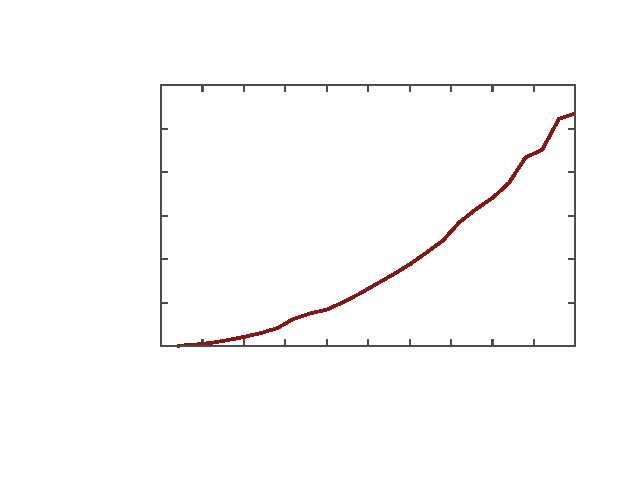
\includegraphics{./graficos/insercion-linux-O0}}%
    \gplfronttext
  \end{picture}%
\endgroup

	\end{center}
\end{frame}

\begin{frame}{Selección}
	Consiste en encontrar el menor de todos los elementos de la lista e intercambiarlo con el de la primera posición. Luego con el segundo, y así sucesivamente hasta ordenarlo todo.
	\vskip 0.5cm
	
	Es $O(n^2)$.
\end{frame}

\begin{frame}
	\begin{center}
		% GNUPLOT: LaTeX picture with Postscript
\begingroup
  \makeatletter
  \providecommand\color[2][]{%
    \GenericError{(gnuplot) \space\space\space\@spaces}{%
      Package color not loaded in conjunction with
      terminal option `colourtext'%
    }{See the gnuplot documentation for explanation.%
    }{Either use 'blacktext' in gnuplot or load the package
      color.sty in LaTeX.}%
    \renewcommand\color[2][]{}%
  }%
  \providecommand\includegraphics[2][]{%
    \GenericError{(gnuplot) \space\space\space\@spaces}{%
      Package graphicx or graphics not loaded%
    }{See the gnuplot documentation for explanation.%
    }{The gnuplot epslatex terminal needs graphicx.sty or graphics.sty.}%
    \renewcommand\includegraphics[2][]{}%
  }%
  \providecommand\rotatebox[2]{#2}%
  \@ifundefined{ifGPcolor}{%
    \newif\ifGPcolor
    \GPcolortrue
  }{}%
  \@ifundefined{ifGPblacktext}{%
    \newif\ifGPblacktext
    \GPblacktextfalse
  }{}%
  % define a \g@addto@macro without @ in the name:
  \let\gplgaddtomacro\g@addto@macro
  % define empty templates for all commands taking text:
  \gdef\gplbacktext{}%
  \gdef\gplfronttext{}%
  \makeatother
  \ifGPblacktext
    % no textcolor at all
    \def\colorrgb#1{}%
    \def\colorgray#1{}%
  \else
    % gray or color?
    \ifGPcolor
      \def\colorrgb#1{\color[rgb]{#1}}%
      \def\colorgray#1{\color[gray]{#1}}%
      \expandafter\def\csname LTw\endcsname{\color{white}}%
      \expandafter\def\csname LTb\endcsname{\color{black}}%
      \expandafter\def\csname LTa\endcsname{\color{black}}%
      \expandafter\def\csname LT0\endcsname{\color[rgb]{1,0,0}}%
      \expandafter\def\csname LT1\endcsname{\color[rgb]{0,1,0}}%
      \expandafter\def\csname LT2\endcsname{\color[rgb]{0,0,1}}%
      \expandafter\def\csname LT3\endcsname{\color[rgb]{1,0,1}}%
      \expandafter\def\csname LT4\endcsname{\color[rgb]{0,1,1}}%
      \expandafter\def\csname LT5\endcsname{\color[rgb]{1,1,0}}%
      \expandafter\def\csname LT6\endcsname{\color[rgb]{0,0,0}}%
      \expandafter\def\csname LT7\endcsname{\color[rgb]{1,0.3,0}}%
      \expandafter\def\csname LT8\endcsname{\color[rgb]{0.5,0.5,0.5}}%
    \else
      % gray
      \def\colorrgb#1{\color{black}}%
      \def\colorgray#1{\color[gray]{#1}}%
      \expandafter\def\csname LTw\endcsname{\color{white}}%
      \expandafter\def\csname LTb\endcsname{\color{black}}%
      \expandafter\def\csname LTa\endcsname{\color{black}}%
      \expandafter\def\csname LT0\endcsname{\color{black}}%
      \expandafter\def\csname LT1\endcsname{\color{black}}%
      \expandafter\def\csname LT2\endcsname{\color{black}}%
      \expandafter\def\csname LT3\endcsname{\color{black}}%
      \expandafter\def\csname LT4\endcsname{\color{black}}%
      \expandafter\def\csname LT5\endcsname{\color{black}}%
      \expandafter\def\csname LT6\endcsname{\color{black}}%
      \expandafter\def\csname LT7\endcsname{\color{black}}%
      \expandafter\def\csname LT8\endcsname{\color{black}}%
    \fi
  \fi
    \setlength{\unitlength}{0.0500bp}%
    \ifx\gptboxheight\undefined%
      \newlength{\gptboxheight}%
      \newlength{\gptboxwidth}%
      \newsavebox{\gptboxtext}%
    \fi%
    \setlength{\fboxrule}{0.5pt}%
    \setlength{\fboxsep}{1pt}%
\begin{picture}(5760.00,4320.00)%
    \gplgaddtomacro\gplbacktext{%
      \colorrgb{0.30,0.30,0.30}%
      \put(1254,1153){\makebox(0,0)[r]{\strut{}$\textcolor{text}{0}$}}%
      \colorrgb{0.30,0.30,0.30}%
      \put(1254,1511){\makebox(0,0)[r]{\strut{}$\textcolor{text}{0.5}$}}%
      \colorrgb{0.30,0.30,0.30}%
      \put(1254,1869){\makebox(0,0)[r]{\strut{}$\textcolor{text}{1}$}}%
      \colorrgb{0.30,0.30,0.30}%
      \put(1254,2227){\makebox(0,0)[r]{\strut{}$\textcolor{text}{1.5}$}}%
      \colorrgb{0.30,0.30,0.30}%
      \put(1254,2585){\makebox(0,0)[r]{\strut{}$\textcolor{text}{2}$}}%
      \colorrgb{0.30,0.30,0.30}%
      \put(1254,2943){\makebox(0,0)[r]{\strut{}$\textcolor{text}{2.5}$}}%
      \colorrgb{0.30,0.30,0.30}%
      \put(1254,3301){\makebox(0,0)[r]{\strut{}$\textcolor{text}{3}$}}%
      \colorrgb{0.30,0.30,0.30}%
      \put(1254,3659){\makebox(0,0)[r]{\strut{}$\textcolor{text}{3.5}$}}%
      \colorrgb{0.30,0.30,0.30}%
      \put(1386,1021){\rotatebox{45}{\makebox(0,0)[r]{\strut{}$\textcolor{text}{0}$}}}%
      \colorrgb{0.30,0.30,0.30}%
      \put(1784,1021){\rotatebox{45}{\makebox(0,0)[r]{\strut{}$\textcolor{text}{5000}$}}}%
      \colorrgb{0.30,0.30,0.30}%
      \put(2181,1021){\rotatebox{45}{\makebox(0,0)[r]{\strut{}$\textcolor{text}{10000}$}}}%
      \colorrgb{0.30,0.30,0.30}%
      \put(2579,1021){\rotatebox{45}{\makebox(0,0)[r]{\strut{}$\textcolor{text}{15000}$}}}%
      \colorrgb{0.30,0.30,0.30}%
      \put(2977,1021){\rotatebox{45}{\makebox(0,0)[r]{\strut{}$\textcolor{text}{20000}$}}}%
      \colorrgb{0.30,0.30,0.30}%
      \put(3375,1021){\rotatebox{45}{\makebox(0,0)[r]{\strut{}$\textcolor{text}{25000}$}}}%
      \colorrgb{0.30,0.30,0.30}%
      \put(3772,1021){\rotatebox{45}{\makebox(0,0)[r]{\strut{}$\textcolor{text}{30000}$}}}%
      \colorrgb{0.30,0.30,0.30}%
      \put(4170,1021){\rotatebox{45}{\makebox(0,0)[r]{\strut{}$\textcolor{text}{35000}$}}}%
      \colorrgb{0.30,0.30,0.30}%
      \put(4568,1021){\rotatebox{45}{\makebox(0,0)[r]{\strut{}$\textcolor{text}{40000}$}}}%
      \colorrgb{0.30,0.30,0.30}%
      \put(4965,1021){\rotatebox{45}{\makebox(0,0)[r]{\strut{}$\textcolor{text}{45000}$}}}%
      \colorrgb{0.30,0.30,0.30}%
      \put(5363,1021){\rotatebox{45}{\makebox(0,0)[r]{\strut{}$\textcolor{text}{50000}$}}}%
    }%
    \gplgaddtomacro\gplfronttext{%
      \colorrgb{0.30,0.30,0.30}%
      \put(220,2406){\rotatebox{-270}{\makebox(0,0){\strut{}Tiempo de ejecución (s)}}}%
      \colorrgb{0.30,0.30,0.30}%
      \put(3374,220){\makebox(0,0){\strut{}Tamaño del vector (elementos)}}%
      \colorrgb{0.30,0.30,0.30}%
      \put(3374,3989){\makebox(0,0){\strut{}seleccion-linux-O0}}%
    }%
    \gplbacktext
    \put(0,0){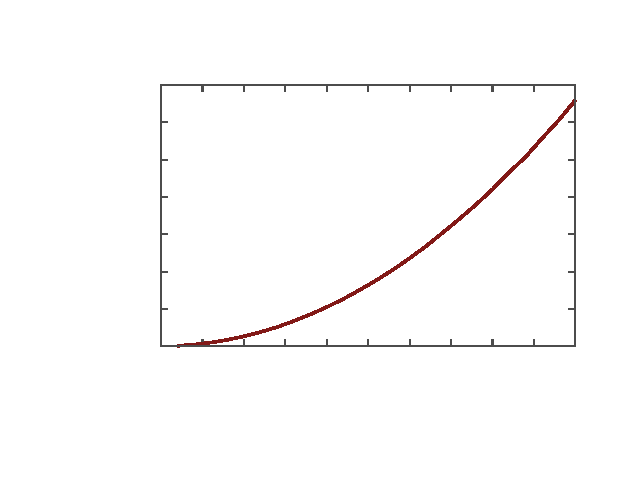
\includegraphics{./graficos/seleccion-linux-O0}}%
    \gplfronttext
  \end{picture}%
\endgroup

	\end{center}
\end{frame}

\begin{frame}{Mergesort}

	Se basa en la técnica de \textit{divide y vencerás}.

	\vskip 0.5cm
	
	\begin{itemize}
		\item Se divide la lista a ordenar en dos sublistas de la mitad de tamaño.
		\item Se ordena cada sublista de forma recursiva.
		\item Si el tamaño de una sublista es 0 o 1 entonces ya está ordenada.
		\item Se unen todas las sublistas en una sola.
	\end{itemize}
	
	\vskip 0.5cm
	
	Es $O(nlogn)$.
\end{frame}

\begin{frame}
	\begin{center}
		% GNUPLOT: LaTeX picture with Postscript
\begingroup
  \makeatletter
  \providecommand\color[2][]{%
    \GenericError{(gnuplot) \space\space\space\@spaces}{%
      Package color not loaded in conjunction with
      terminal option `colourtext'%
    }{See the gnuplot documentation for explanation.%
    }{Either use 'blacktext' in gnuplot or load the package
      color.sty in LaTeX.}%
    \renewcommand\color[2][]{}%
  }%
  \providecommand\includegraphics[2][]{%
    \GenericError{(gnuplot) \space\space\space\@spaces}{%
      Package graphicx or graphics not loaded%
    }{See the gnuplot documentation for explanation.%
    }{The gnuplot epslatex terminal needs graphicx.sty or graphics.sty.}%
    \renewcommand\includegraphics[2][]{}%
  }%
  \providecommand\rotatebox[2]{#2}%
  \@ifundefined{ifGPcolor}{%
    \newif\ifGPcolor
    \GPcolortrue
  }{}%
  \@ifundefined{ifGPblacktext}{%
    \newif\ifGPblacktext
    \GPblacktextfalse
  }{}%
  % define a \g@addto@macro without @ in the name:
  \let\gplgaddtomacro\g@addto@macro
  % define empty templates for all commands taking text:
  \gdef\gplbacktext{}%
  \gdef\gplfronttext{}%
  \makeatother
  \ifGPblacktext
    % no textcolor at all
    \def\colorrgb#1{}%
    \def\colorgray#1{}%
  \else
    % gray or color?
    \ifGPcolor
      \def\colorrgb#1{\color[rgb]{#1}}%
      \def\colorgray#1{\color[gray]{#1}}%
      \expandafter\def\csname LTw\endcsname{\color{white}}%
      \expandafter\def\csname LTb\endcsname{\color{black}}%
      \expandafter\def\csname LTa\endcsname{\color{black}}%
      \expandafter\def\csname LT0\endcsname{\color[rgb]{1,0,0}}%
      \expandafter\def\csname LT1\endcsname{\color[rgb]{0,1,0}}%
      \expandafter\def\csname LT2\endcsname{\color[rgb]{0,0,1}}%
      \expandafter\def\csname LT3\endcsname{\color[rgb]{1,0,1}}%
      \expandafter\def\csname LT4\endcsname{\color[rgb]{0,1,1}}%
      \expandafter\def\csname LT5\endcsname{\color[rgb]{1,1,0}}%
      \expandafter\def\csname LT6\endcsname{\color[rgb]{0,0,0}}%
      \expandafter\def\csname LT7\endcsname{\color[rgb]{1,0.3,0}}%
      \expandafter\def\csname LT8\endcsname{\color[rgb]{0.5,0.5,0.5}}%
    \else
      % gray
      \def\colorrgb#1{\color{black}}%
      \def\colorgray#1{\color[gray]{#1}}%
      \expandafter\def\csname LTw\endcsname{\color{white}}%
      \expandafter\def\csname LTb\endcsname{\color{black}}%
      \expandafter\def\csname LTa\endcsname{\color{black}}%
      \expandafter\def\csname LT0\endcsname{\color{black}}%
      \expandafter\def\csname LT1\endcsname{\color{black}}%
      \expandafter\def\csname LT2\endcsname{\color{black}}%
      \expandafter\def\csname LT3\endcsname{\color{black}}%
      \expandafter\def\csname LT4\endcsname{\color{black}}%
      \expandafter\def\csname LT5\endcsname{\color{black}}%
      \expandafter\def\csname LT6\endcsname{\color{black}}%
      \expandafter\def\csname LT7\endcsname{\color{black}}%
      \expandafter\def\csname LT8\endcsname{\color{black}}%
    \fi
  \fi
    \setlength{\unitlength}{0.0500bp}%
    \ifx\gptboxheight\undefined%
      \newlength{\gptboxheight}%
      \newlength{\gptboxwidth}%
      \newsavebox{\gptboxtext}%
    \fi%
    \setlength{\fboxrule}{0.5pt}%
    \setlength{\fboxsep}{1pt}%
\begin{picture}(5760.00,4320.00)%
    \gplgaddtomacro\gplbacktext{%
      \colorrgb{0.30,0.30,0.30}%
      \put(1518,1246){\makebox(0,0)[r]{\strut{}$\textcolor{text}{0}$}}%
      \colorrgb{0.30,0.30,0.30}%
      \put(1518,1591){\makebox(0,0)[r]{\strut{}$\textcolor{text}{0.005}$}}%
      \colorrgb{0.30,0.30,0.30}%
      \put(1518,1935){\makebox(0,0)[r]{\strut{}$\textcolor{text}{0.01}$}}%
      \colorrgb{0.30,0.30,0.30}%
      \put(1518,2280){\makebox(0,0)[r]{\strut{}$\textcolor{text}{0.015}$}}%
      \colorrgb{0.30,0.30,0.30}%
      \put(1518,2625){\makebox(0,0)[r]{\strut{}$\textcolor{text}{0.02}$}}%
      \colorrgb{0.30,0.30,0.30}%
      \put(1518,2970){\makebox(0,0)[r]{\strut{}$\textcolor{text}{0.025}$}}%
      \colorrgb{0.30,0.30,0.30}%
      \put(1518,3314){\makebox(0,0)[r]{\strut{}$\textcolor{text}{0.03}$}}%
      \colorrgb{0.30,0.30,0.30}%
      \put(1518,3659){\makebox(0,0)[r]{\strut{}$\textcolor{text}{0.035}$}}%
      \colorrgb{0.30,0.30,0.30}%
      \put(1650,1114){\rotatebox{45}{\makebox(0,0)[r]{\strut{}$\textcolor{text}{0}$}}}%
      \colorrgb{0.30,0.30,0.30}%
      \put(2114,1114){\rotatebox{45}{\makebox(0,0)[r]{\strut{}$\textcolor{text}{20000}$}}}%
      \colorrgb{0.30,0.30,0.30}%
      \put(2578,1114){\rotatebox{45}{\makebox(0,0)[r]{\strut{}$\textcolor{text}{40000}$}}}%
      \colorrgb{0.30,0.30,0.30}%
      \put(3042,1114){\rotatebox{45}{\makebox(0,0)[r]{\strut{}$\textcolor{text}{60000}$}}}%
      \colorrgb{0.30,0.30,0.30}%
      \put(3507,1114){\rotatebox{45}{\makebox(0,0)[r]{\strut{}$\textcolor{text}{80000}$}}}%
      \colorrgb{0.30,0.30,0.30}%
      \put(3971,1114){\rotatebox{45}{\makebox(0,0)[r]{\strut{}$\textcolor{text}{100000}$}}}%
      \colorrgb{0.30,0.30,0.30}%
      \put(4435,1114){\rotatebox{45}{\makebox(0,0)[r]{\strut{}$\textcolor{text}{120000}$}}}%
      \colorrgb{0.30,0.30,0.30}%
      \put(4899,1114){\rotatebox{45}{\makebox(0,0)[r]{\strut{}$\textcolor{text}{140000}$}}}%
      \colorrgb{0.30,0.30,0.30}%
      \put(5363,1114){\rotatebox{45}{\makebox(0,0)[r]{\strut{}$\textcolor{text}{160000}$}}}%
    }%
    \gplgaddtomacro\gplfronttext{%
      \colorrgb{0.30,0.30,0.30}%
      \put(220,2452){\rotatebox{-270}{\makebox(0,0){\strut{}Tiempo de ejecución (s)}}}%
      \colorrgb{0.30,0.30,0.30}%
      \put(3506,220){\makebox(0,0){\strut{}Tamaño del vector (elementos)}}%
      \colorrgb{0.30,0.30,0.30}%
      \put(3506,3989){\makebox(0,0){\strut{}mergesort-linux-O0}}%
    }%
    \gplbacktext
    \put(0,0){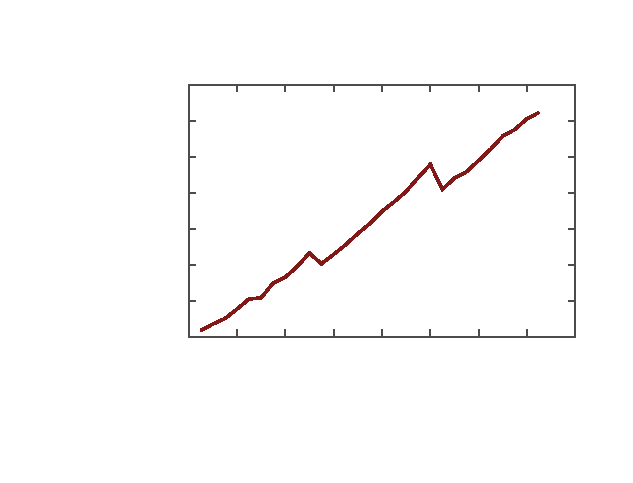
\includegraphics{./graficos/mergesort-linux-O0}}%
    \gplfronttext
  \end{picture}%
\endgroup

	\end{center}
\end{frame}

\begin{frame}{Quicksort}

	Se basa en la técnica de \textit{divide y vencerás}.

	\vskip 0.5cm
	
	\begin{itemize}
		\item Elegimos un elemento de la lista, el \textit{pivote}.
		\item Se ordena la lista, dejando los elementos mayores a la derecha del pivote y los menores a la izquierda.
		\item Realizamos el proceso recursivamente en las dos sublistas que nos quedan (derecha e izquierda) hasta que tengan 0 o 1 elemento.
	\end{itemize}
	
	\vskip 0.5cm
	
	Es $O(nlogn)$.
\end{frame}

\begin{frame}
	\begin{center}
		% GNUPLOT: LaTeX picture with Postscript
\begingroup
  \makeatletter
  \providecommand\color[2][]{%
    \GenericError{(gnuplot) \space\space\space\@spaces}{%
      Package color not loaded in conjunction with
      terminal option `colourtext'%
    }{See the gnuplot documentation for explanation.%
    }{Either use 'blacktext' in gnuplot or load the package
      color.sty in LaTeX.}%
    \renewcommand\color[2][]{}%
  }%
  \providecommand\includegraphics[2][]{%
    \GenericError{(gnuplot) \space\space\space\@spaces}{%
      Package graphicx or graphics not loaded%
    }{See the gnuplot documentation for explanation.%
    }{The gnuplot epslatex terminal needs graphicx.sty or graphics.sty.}%
    \renewcommand\includegraphics[2][]{}%
  }%
  \providecommand\rotatebox[2]{#2}%
  \@ifundefined{ifGPcolor}{%
    \newif\ifGPcolor
    \GPcolortrue
  }{}%
  \@ifundefined{ifGPblacktext}{%
    \newif\ifGPblacktext
    \GPblacktextfalse
  }{}%
  % define a \g@addto@macro without @ in the name:
  \let\gplgaddtomacro\g@addto@macro
  % define empty templates for all commands taking text:
  \gdef\gplbacktext{}%
  \gdef\gplfronttext{}%
  \makeatother
  \ifGPblacktext
    % no textcolor at all
    \def\colorrgb#1{}%
    \def\colorgray#1{}%
  \else
    % gray or color?
    \ifGPcolor
      \def\colorrgb#1{\color[rgb]{#1}}%
      \def\colorgray#1{\color[gray]{#1}}%
      \expandafter\def\csname LTw\endcsname{\color{white}}%
      \expandafter\def\csname LTb\endcsname{\color{black}}%
      \expandafter\def\csname LTa\endcsname{\color{black}}%
      \expandafter\def\csname LT0\endcsname{\color[rgb]{1,0,0}}%
      \expandafter\def\csname LT1\endcsname{\color[rgb]{0,1,0}}%
      \expandafter\def\csname LT2\endcsname{\color[rgb]{0,0,1}}%
      \expandafter\def\csname LT3\endcsname{\color[rgb]{1,0,1}}%
      \expandafter\def\csname LT4\endcsname{\color[rgb]{0,1,1}}%
      \expandafter\def\csname LT5\endcsname{\color[rgb]{1,1,0}}%
      \expandafter\def\csname LT6\endcsname{\color[rgb]{0,0,0}}%
      \expandafter\def\csname LT7\endcsname{\color[rgb]{1,0.3,0}}%
      \expandafter\def\csname LT8\endcsname{\color[rgb]{0.5,0.5,0.5}}%
    \else
      % gray
      \def\colorrgb#1{\color{black}}%
      \def\colorgray#1{\color[gray]{#1}}%
      \expandafter\def\csname LTw\endcsname{\color{white}}%
      \expandafter\def\csname LTb\endcsname{\color{black}}%
      \expandafter\def\csname LTa\endcsname{\color{black}}%
      \expandafter\def\csname LT0\endcsname{\color{black}}%
      \expandafter\def\csname LT1\endcsname{\color{black}}%
      \expandafter\def\csname LT2\endcsname{\color{black}}%
      \expandafter\def\csname LT3\endcsname{\color{black}}%
      \expandafter\def\csname LT4\endcsname{\color{black}}%
      \expandafter\def\csname LT5\endcsname{\color{black}}%
      \expandafter\def\csname LT6\endcsname{\color{black}}%
      \expandafter\def\csname LT7\endcsname{\color{black}}%
      \expandafter\def\csname LT8\endcsname{\color{black}}%
    \fi
  \fi
    \setlength{\unitlength}{0.0500bp}%
    \ifx\gptboxheight\undefined%
      \newlength{\gptboxheight}%
      \newlength{\gptboxwidth}%
      \newsavebox{\gptboxtext}%
    \fi%
    \setlength{\fboxrule}{0.5pt}%
    \setlength{\fboxsep}{1pt}%
\begin{picture}(5760.00,4320.00)%
    \gplgaddtomacro\gplbacktext{%
      \colorrgb{0.30,0.30,0.30}%
      \put(1650,1246){\makebox(0,0)[r]{\strut{}$\textcolor{text}{0.0001}$}}%
      \colorrgb{0.30,0.30,0.30}%
      \put(1650,2050){\makebox(0,0)[r]{\strut{}$\textcolor{text}{0.001}$}}%
      \colorrgb{0.30,0.30,0.30}%
      \put(1650,2855){\makebox(0,0)[r]{\strut{}$\textcolor{text}{0.01}$}}%
      \colorrgb{0.30,0.30,0.30}%
      \put(1650,3659){\makebox(0,0)[r]{\strut{}$\textcolor{text}{0.1}$}}%
      \colorrgb{0.30,0.30,0.30}%
      \put(1782,1114){\rotatebox{45}{\makebox(0,0)[r]{\strut{}$\textcolor{text}{0}$}}}%
      \colorrgb{0.30,0.30,0.30}%
      \put(2230,1114){\rotatebox{45}{\makebox(0,0)[r]{\strut{}$\textcolor{text}{20000}$}}}%
      \colorrgb{0.30,0.30,0.30}%
      \put(2677,1114){\rotatebox{45}{\makebox(0,0)[r]{\strut{}$\textcolor{text}{40000}$}}}%
      \colorrgb{0.30,0.30,0.30}%
      \put(3125,1114){\rotatebox{45}{\makebox(0,0)[r]{\strut{}$\textcolor{text}{60000}$}}}%
      \colorrgb{0.30,0.30,0.30}%
      \put(3573,1114){\rotatebox{45}{\makebox(0,0)[r]{\strut{}$\textcolor{text}{80000}$}}}%
      \colorrgb{0.30,0.30,0.30}%
      \put(4020,1114){\rotatebox{45}{\makebox(0,0)[r]{\strut{}$\textcolor{text}{100000}$}}}%
      \colorrgb{0.30,0.30,0.30}%
      \put(4468,1114){\rotatebox{45}{\makebox(0,0)[r]{\strut{}$\textcolor{text}{120000}$}}}%
      \colorrgb{0.30,0.30,0.30}%
      \put(4915,1114){\rotatebox{45}{\makebox(0,0)[r]{\strut{}$\textcolor{text}{140000}$}}}%
      \colorrgb{0.30,0.30,0.30}%
      \put(5363,1114){\rotatebox{45}{\makebox(0,0)[r]{\strut{}$\textcolor{text}{160000}$}}}%
    }%
    \gplgaddtomacro\gplfronttext{%
      \colorrgb{0.30,0.30,0.30}%
      \put(220,2452){\rotatebox{-270}{\makebox(0,0){\strut{}Tiempo de ejecución (s)}}}%
      \colorrgb{0.30,0.30,0.30}%
      \put(3572,220){\makebox(0,0){\strut{}Tamaño del vector (elementos)}}%
      \colorrgb{0.30,0.30,0.30}%
      \put(3572,3989){\makebox(0,0){\strut{}quicksort-linux-O0}}%
    }%
    \gplbacktext
    \put(0,0){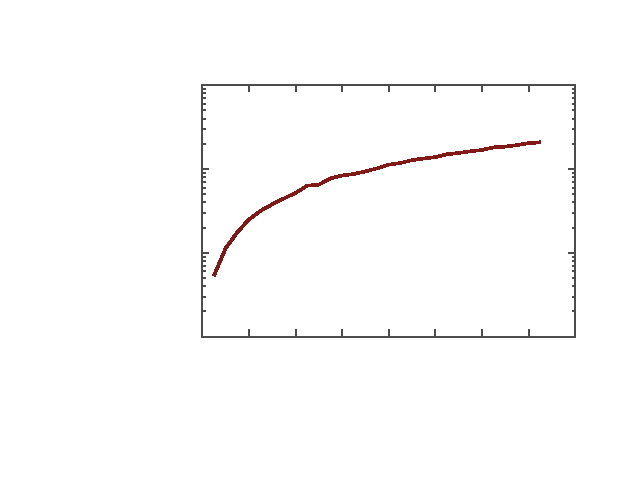
\includegraphics{./graficos/quicksort-linux-O0}}%
    \gplfronttext
  \end{picture}%
\endgroup

	\end{center}
\end{frame}

\begin{frame}{Heapsort}

	Es un método de ordenación por selección.

	\vskip 0.5cm
	
	\begin{itemize}
		\item El \textit{heap} es un árbol binario de altura mínima, en el que los nodos del nivel más bajo están lo más a la izquierda posible.
		\item Los hijos de cada nodo son siempre menores que el padre.
		\item No es necesario recorrer el árbol de forma desordenada para encontrar los elementos máximos.
	\end{itemize}
	
	\vskip 0.5cm
	
	Es $O(nlogn)$.
\end{frame}


\begin{frame}
	\begin{center}
		% GNUPLOT: LaTeX picture with Postscript
\begingroup
  \makeatletter
  \providecommand\color[2][]{%
    \GenericError{(gnuplot) \space\space\space\@spaces}{%
      Package color not loaded in conjunction with
      terminal option `colourtext'%
    }{See the gnuplot documentation for explanation.%
    }{Either use 'blacktext' in gnuplot or load the package
      color.sty in LaTeX.}%
    \renewcommand\color[2][]{}%
  }%
  \providecommand\includegraphics[2][]{%
    \GenericError{(gnuplot) \space\space\space\@spaces}{%
      Package graphicx or graphics not loaded%
    }{See the gnuplot documentation for explanation.%
    }{The gnuplot epslatex terminal needs graphicx.sty or graphics.sty.}%
    \renewcommand\includegraphics[2][]{}%
  }%
  \providecommand\rotatebox[2]{#2}%
  \@ifundefined{ifGPcolor}{%
    \newif\ifGPcolor
    \GPcolortrue
  }{}%
  \@ifundefined{ifGPblacktext}{%
    \newif\ifGPblacktext
    \GPblacktextfalse
  }{}%
  % define a \g@addto@macro without @ in the name:
  \let\gplgaddtomacro\g@addto@macro
  % define empty templates for all commands taking text:
  \gdef\gplbacktext{}%
  \gdef\gplfronttext{}%
  \makeatother
  \ifGPblacktext
    % no textcolor at all
    \def\colorrgb#1{}%
    \def\colorgray#1{}%
  \else
    % gray or color?
    \ifGPcolor
      \def\colorrgb#1{\color[rgb]{#1}}%
      \def\colorgray#1{\color[gray]{#1}}%
      \expandafter\def\csname LTw\endcsname{\color{white}}%
      \expandafter\def\csname LTb\endcsname{\color{black}}%
      \expandafter\def\csname LTa\endcsname{\color{black}}%
      \expandafter\def\csname LT0\endcsname{\color[rgb]{1,0,0}}%
      \expandafter\def\csname LT1\endcsname{\color[rgb]{0,1,0}}%
      \expandafter\def\csname LT2\endcsname{\color[rgb]{0,0,1}}%
      \expandafter\def\csname LT3\endcsname{\color[rgb]{1,0,1}}%
      \expandafter\def\csname LT4\endcsname{\color[rgb]{0,1,1}}%
      \expandafter\def\csname LT5\endcsname{\color[rgb]{1,1,0}}%
      \expandafter\def\csname LT6\endcsname{\color[rgb]{0,0,0}}%
      \expandafter\def\csname LT7\endcsname{\color[rgb]{1,0.3,0}}%
      \expandafter\def\csname LT8\endcsname{\color[rgb]{0.5,0.5,0.5}}%
    \else
      % gray
      \def\colorrgb#1{\color{black}}%
      \def\colorgray#1{\color[gray]{#1}}%
      \expandafter\def\csname LTw\endcsname{\color{white}}%
      \expandafter\def\csname LTb\endcsname{\color{black}}%
      \expandafter\def\csname LTa\endcsname{\color{black}}%
      \expandafter\def\csname LT0\endcsname{\color{black}}%
      \expandafter\def\csname LT1\endcsname{\color{black}}%
      \expandafter\def\csname LT2\endcsname{\color{black}}%
      \expandafter\def\csname LT3\endcsname{\color{black}}%
      \expandafter\def\csname LT4\endcsname{\color{black}}%
      \expandafter\def\csname LT5\endcsname{\color{black}}%
      \expandafter\def\csname LT6\endcsname{\color{black}}%
      \expandafter\def\csname LT7\endcsname{\color{black}}%
      \expandafter\def\csname LT8\endcsname{\color{black}}%
    \fi
  \fi
    \setlength{\unitlength}{0.0500bp}%
    \ifx\gptboxheight\undefined%
      \newlength{\gptboxheight}%
      \newlength{\gptboxwidth}%
      \newsavebox{\gptboxtext}%
    \fi%
    \setlength{\fboxrule}{0.5pt}%
    \setlength{\fboxsep}{1pt}%
\begin{picture}(5760.00,4320.00)%
    \gplgaddtomacro\gplbacktext{%
      \colorrgb{0.30,0.30,0.30}%
      \put(1650,1246){\makebox(0,0)[r]{\strut{}$\textcolor{text}{0.0001}$}}%
      \colorrgb{0.30,0.30,0.30}%
      \put(1650,2050){\makebox(0,0)[r]{\strut{}$\textcolor{text}{0.001}$}}%
      \colorrgb{0.30,0.30,0.30}%
      \put(1650,2855){\makebox(0,0)[r]{\strut{}$\textcolor{text}{0.01}$}}%
      \colorrgb{0.30,0.30,0.30}%
      \put(1650,3659){\makebox(0,0)[r]{\strut{}$\textcolor{text}{0.1}$}}%
      \colorrgb{0.30,0.30,0.30}%
      \put(1782,1114){\rotatebox{45}{\makebox(0,0)[r]{\strut{}$\textcolor{text}{0}$}}}%
      \colorrgb{0.30,0.30,0.30}%
      \put(2230,1114){\rotatebox{45}{\makebox(0,0)[r]{\strut{}$\textcolor{text}{20000}$}}}%
      \colorrgb{0.30,0.30,0.30}%
      \put(2677,1114){\rotatebox{45}{\makebox(0,0)[r]{\strut{}$\textcolor{text}{40000}$}}}%
      \colorrgb{0.30,0.30,0.30}%
      \put(3125,1114){\rotatebox{45}{\makebox(0,0)[r]{\strut{}$\textcolor{text}{60000}$}}}%
      \colorrgb{0.30,0.30,0.30}%
      \put(3573,1114){\rotatebox{45}{\makebox(0,0)[r]{\strut{}$\textcolor{text}{80000}$}}}%
      \colorrgb{0.30,0.30,0.30}%
      \put(4020,1114){\rotatebox{45}{\makebox(0,0)[r]{\strut{}$\textcolor{text}{100000}$}}}%
      \colorrgb{0.30,0.30,0.30}%
      \put(4468,1114){\rotatebox{45}{\makebox(0,0)[r]{\strut{}$\textcolor{text}{120000}$}}}%
      \colorrgb{0.30,0.30,0.30}%
      \put(4915,1114){\rotatebox{45}{\makebox(0,0)[r]{\strut{}$\textcolor{text}{140000}$}}}%
      \colorrgb{0.30,0.30,0.30}%
      \put(5363,1114){\rotatebox{45}{\makebox(0,0)[r]{\strut{}$\textcolor{text}{160000}$}}}%
    }%
    \gplgaddtomacro\gplfronttext{%
      \colorrgb{0.30,0.30,0.30}%
      \put(220,2452){\rotatebox{-270}{\makebox(0,0){\strut{}Tiempo de ejecución (s)}}}%
      \colorrgb{0.30,0.30,0.30}%
      \put(3572,220){\makebox(0,0){\strut{}Tamaño del vector (elementos)}}%
      \colorrgb{0.30,0.30,0.30}%
      \put(3572,3989){\makebox(0,0){\strut{}heapsort-linux-O0}}%
    }%
    \gplbacktext
    \put(0,0){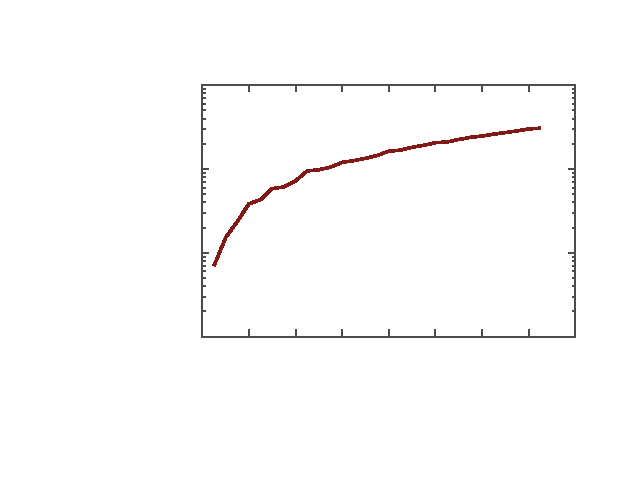
\includegraphics{./graficos/heapsort-linux-O0}}%
    \gplfronttext
  \end{picture}%
\endgroup

	\end{center}
\end{frame}

\begin{frame}{Floyd}

	Algoritmo de análisis sobre grafos para encontrar el camino mínimo en grafos ponderados.

	\vskip 0.5cm
	
	\begin{itemize}
		\item El algoritmo compara todos los posibles caminos a través del grafo entre cada par de vértices.
	\end{itemize}
	
	\vskip 0.5cm
	
	Es $O(n^3)$.
\end{frame}

\begin{frame}
	\begin{center}
		% GNUPLOT: LaTeX picture with Postscript
\begingroup
  \makeatletter
  \providecommand\color[2][]{%
    \GenericError{(gnuplot) \space\space\space\@spaces}{%
      Package color not loaded in conjunction with
      terminal option `colourtext'%
    }{See the gnuplot documentation for explanation.%
    }{Either use 'blacktext' in gnuplot or load the package
      color.sty in LaTeX.}%
    \renewcommand\color[2][]{}%
  }%
  \providecommand\includegraphics[2][]{%
    \GenericError{(gnuplot) \space\space\space\@spaces}{%
      Package graphicx or graphics not loaded%
    }{See the gnuplot documentation for explanation.%
    }{The gnuplot epslatex terminal needs graphicx.sty or graphics.sty.}%
    \renewcommand\includegraphics[2][]{}%
  }%
  \providecommand\rotatebox[2]{#2}%
  \@ifundefined{ifGPcolor}{%
    \newif\ifGPcolor
    \GPcolortrue
  }{}%
  \@ifundefined{ifGPblacktext}{%
    \newif\ifGPblacktext
    \GPblacktextfalse
  }{}%
  % define a \g@addto@macro without @ in the name:
  \let\gplgaddtomacro\g@addto@macro
  % define empty templates for all commands taking text:
  \gdef\gplbacktext{}%
  \gdef\gplfronttext{}%
  \makeatother
  \ifGPblacktext
    % no textcolor at all
    \def\colorrgb#1{}%
    \def\colorgray#1{}%
  \else
    % gray or color?
    \ifGPcolor
      \def\colorrgb#1{\color[rgb]{#1}}%
      \def\colorgray#1{\color[gray]{#1}}%
      \expandafter\def\csname LTw\endcsname{\color{white}}%
      \expandafter\def\csname LTb\endcsname{\color{black}}%
      \expandafter\def\csname LTa\endcsname{\color{black}}%
      \expandafter\def\csname LT0\endcsname{\color[rgb]{1,0,0}}%
      \expandafter\def\csname LT1\endcsname{\color[rgb]{0,1,0}}%
      \expandafter\def\csname LT2\endcsname{\color[rgb]{0,0,1}}%
      \expandafter\def\csname LT3\endcsname{\color[rgb]{1,0,1}}%
      \expandafter\def\csname LT4\endcsname{\color[rgb]{0,1,1}}%
      \expandafter\def\csname LT5\endcsname{\color[rgb]{1,1,0}}%
      \expandafter\def\csname LT6\endcsname{\color[rgb]{0,0,0}}%
      \expandafter\def\csname LT7\endcsname{\color[rgb]{1,0.3,0}}%
      \expandafter\def\csname LT8\endcsname{\color[rgb]{0.5,0.5,0.5}}%
    \else
      % gray
      \def\colorrgb#1{\color{black}}%
      \def\colorgray#1{\color[gray]{#1}}%
      \expandafter\def\csname LTw\endcsname{\color{white}}%
      \expandafter\def\csname LTb\endcsname{\color{black}}%
      \expandafter\def\csname LTa\endcsname{\color{black}}%
      \expandafter\def\csname LT0\endcsname{\color{black}}%
      \expandafter\def\csname LT1\endcsname{\color{black}}%
      \expandafter\def\csname LT2\endcsname{\color{black}}%
      \expandafter\def\csname LT3\endcsname{\color{black}}%
      \expandafter\def\csname LT4\endcsname{\color{black}}%
      \expandafter\def\csname LT5\endcsname{\color{black}}%
      \expandafter\def\csname LT6\endcsname{\color{black}}%
      \expandafter\def\csname LT7\endcsname{\color{black}}%
      \expandafter\def\csname LT8\endcsname{\color{black}}%
    \fi
  \fi
    \setlength{\unitlength}{0.0500bp}%
    \ifx\gptboxheight\undefined%
      \newlength{\gptboxheight}%
      \newlength{\gptboxwidth}%
      \newsavebox{\gptboxtext}%
    \fi%
    \setlength{\fboxrule}{0.5pt}%
    \setlength{\fboxsep}{1pt}%
\begin{picture}(5760.00,4320.00)%
    \gplgaddtomacro\gplbacktext{%
      \colorrgb{0.30,0.30,0.30}%
      \put(1122,1060){\makebox(0,0)[r]{\strut{}$\textcolor{text}{0}$}}%
      \colorrgb{0.30,0.30,0.30}%
      \put(1122,1349){\makebox(0,0)[r]{\strut{}$\textcolor{text}{2}$}}%
      \colorrgb{0.30,0.30,0.30}%
      \put(1122,1638){\makebox(0,0)[r]{\strut{}$\textcolor{text}{4}$}}%
      \colorrgb{0.30,0.30,0.30}%
      \put(1122,1926){\makebox(0,0)[r]{\strut{}$\textcolor{text}{6}$}}%
      \colorrgb{0.30,0.30,0.30}%
      \put(1122,2215){\makebox(0,0)[r]{\strut{}$\textcolor{text}{8}$}}%
      \colorrgb{0.30,0.30,0.30}%
      \put(1122,2504){\makebox(0,0)[r]{\strut{}$\textcolor{text}{10}$}}%
      \colorrgb{0.30,0.30,0.30}%
      \put(1122,2793){\makebox(0,0)[r]{\strut{}$\textcolor{text}{12}$}}%
      \colorrgb{0.30,0.30,0.30}%
      \put(1122,3081){\makebox(0,0)[r]{\strut{}$\textcolor{text}{14}$}}%
      \colorrgb{0.30,0.30,0.30}%
      \put(1122,3370){\makebox(0,0)[r]{\strut{}$\textcolor{text}{16}$}}%
      \colorrgb{0.30,0.30,0.30}%
      \put(1122,3659){\makebox(0,0)[r]{\strut{}$\textcolor{text}{18}$}}%
      \colorrgb{0.30,0.30,0.30}%
      \put(1254,928){\rotatebox{45}{\makebox(0,0)[r]{\strut{}$\textcolor{text}{0}$}}}%
      \colorrgb{0.30,0.30,0.30}%
      \put(1768,928){\rotatebox{45}{\makebox(0,0)[r]{\strut{}$\textcolor{text}{200}$}}}%
      \colorrgb{0.30,0.30,0.30}%
      \put(2281,928){\rotatebox{45}{\makebox(0,0)[r]{\strut{}$\textcolor{text}{400}$}}}%
      \colorrgb{0.30,0.30,0.30}%
      \put(2795,928){\rotatebox{45}{\makebox(0,0)[r]{\strut{}$\textcolor{text}{600}$}}}%
      \colorrgb{0.30,0.30,0.30}%
      \put(3309,928){\rotatebox{45}{\makebox(0,0)[r]{\strut{}$\textcolor{text}{800}$}}}%
      \colorrgb{0.30,0.30,0.30}%
      \put(3822,928){\rotatebox{45}{\makebox(0,0)[r]{\strut{}$\textcolor{text}{1000}$}}}%
      \colorrgb{0.30,0.30,0.30}%
      \put(4336,928){\rotatebox{45}{\makebox(0,0)[r]{\strut{}$\textcolor{text}{1200}$}}}%
      \colorrgb{0.30,0.30,0.30}%
      \put(4849,928){\rotatebox{45}{\makebox(0,0)[r]{\strut{}$\textcolor{text}{1400}$}}}%
      \colorrgb{0.30,0.30,0.30}%
      \put(5363,928){\rotatebox{45}{\makebox(0,0)[r]{\strut{}$\textcolor{text}{1600}$}}}%
    }%
    \gplgaddtomacro\gplfronttext{%
      \colorrgb{0.30,0.30,0.30}%
      \put(220,2359){\rotatebox{-270}{\makebox(0,0){\strut{}Tiempo de ejecución (s)}}}%
      \colorrgb{0.30,0.30,0.30}%
      \put(3308,220){\makebox(0,0){\strut{}Tamaño del grafo (vértices)}}%
      \colorrgb{0.30,0.30,0.30}%
      \put(3308,3989){\makebox(0,0){\strut{}Eficiencia empírica floyd-linux-O0}}%
    }%
    \gplbacktext
    \put(0,0){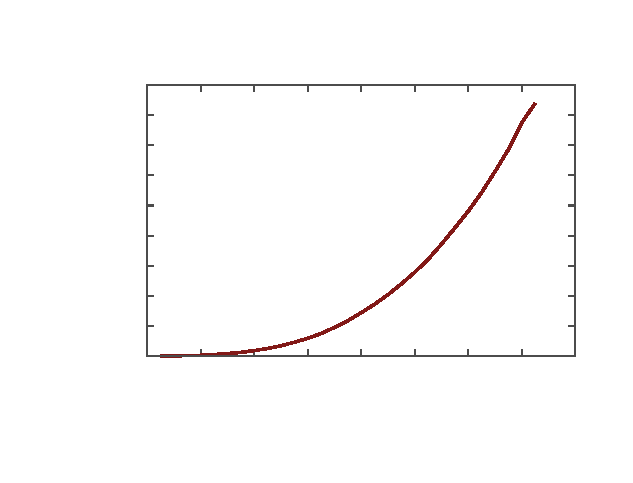
\includegraphics{./graficos/floyd-linux-O0}}%
    \gplfronttext
  \end{picture}%
\endgroup

	\end{center}
\end{frame}

\begin{frame}{Hanoi}

	Las torres de Hanoi son un puzzle matemático.

	\vskip 0.5cm
	
	\begin{itemize}
		\item Tenemos 3 pilas: origen, auxiliar y destino.
		\item Origen está ordenada por tamaño creciente de discos.
		\item Se mueve un disco de la pila origen a la de destino si hay un único disco en la pila origen.
		\item Si no, se mueven todos los discos a la auxiliar, excepto el más grande.
		\item Por último, movemos el disco mayor al destino, y los $n-1$ restantes encima del mayor.
	\end{itemize}
	
	\vskip 0.5cm
	
	Es $O(2^n)$.
\end{frame}

\begin{frame}
	\begin{center}
		% GNUPLOT: LaTeX picture with Postscript
\begingroup
  \makeatletter
  \providecommand\color[2][]{%
    \GenericError{(gnuplot) \space\space\space\@spaces}{%
      Package color not loaded in conjunction with
      terminal option `colourtext'%
    }{See the gnuplot documentation for explanation.%
    }{Either use 'blacktext' in gnuplot or load the package
      color.sty in LaTeX.}%
    \renewcommand\color[2][]{}%
  }%
  \providecommand\includegraphics[2][]{%
    \GenericError{(gnuplot) \space\space\space\@spaces}{%
      Package graphicx or graphics not loaded%
    }{See the gnuplot documentation for explanation.%
    }{The gnuplot epslatex terminal needs graphicx.sty or graphics.sty.}%
    \renewcommand\includegraphics[2][]{}%
  }%
  \providecommand\rotatebox[2]{#2}%
  \@ifundefined{ifGPcolor}{%
    \newif\ifGPcolor
    \GPcolortrue
  }{}%
  \@ifundefined{ifGPblacktext}{%
    \newif\ifGPblacktext
    \GPblacktextfalse
  }{}%
  % define a \g@addto@macro without @ in the name:
  \let\gplgaddtomacro\g@addto@macro
  % define empty templates for all commands taking text:
  \gdef\gplbacktext{}%
  \gdef\gplfronttext{}%
  \makeatother
  \ifGPblacktext
    % no textcolor at all
    \def\colorrgb#1{}%
    \def\colorgray#1{}%
  \else
    % gray or color?
    \ifGPcolor
      \def\colorrgb#1{\color[rgb]{#1}}%
      \def\colorgray#1{\color[gray]{#1}}%
      \expandafter\def\csname LTw\endcsname{\color{white}}%
      \expandafter\def\csname LTb\endcsname{\color{black}}%
      \expandafter\def\csname LTa\endcsname{\color{black}}%
      \expandafter\def\csname LT0\endcsname{\color[rgb]{1,0,0}}%
      \expandafter\def\csname LT1\endcsname{\color[rgb]{0,1,0}}%
      \expandafter\def\csname LT2\endcsname{\color[rgb]{0,0,1}}%
      \expandafter\def\csname LT3\endcsname{\color[rgb]{1,0,1}}%
      \expandafter\def\csname LT4\endcsname{\color[rgb]{0,1,1}}%
      \expandafter\def\csname LT5\endcsname{\color[rgb]{1,1,0}}%
      \expandafter\def\csname LT6\endcsname{\color[rgb]{0,0,0}}%
      \expandafter\def\csname LT7\endcsname{\color[rgb]{1,0.3,0}}%
      \expandafter\def\csname LT8\endcsname{\color[rgb]{0.5,0.5,0.5}}%
    \else
      % gray
      \def\colorrgb#1{\color{black}}%
      \def\colorgray#1{\color[gray]{#1}}%
      \expandafter\def\csname LTw\endcsname{\color{white}}%
      \expandafter\def\csname LTb\endcsname{\color{black}}%
      \expandafter\def\csname LTa\endcsname{\color{black}}%
      \expandafter\def\csname LT0\endcsname{\color{black}}%
      \expandafter\def\csname LT1\endcsname{\color{black}}%
      \expandafter\def\csname LT2\endcsname{\color{black}}%
      \expandafter\def\csname LT3\endcsname{\color{black}}%
      \expandafter\def\csname LT4\endcsname{\color{black}}%
      \expandafter\def\csname LT5\endcsname{\color{black}}%
      \expandafter\def\csname LT6\endcsname{\color{black}}%
      \expandafter\def\csname LT7\endcsname{\color{black}}%
      \expandafter\def\csname LT8\endcsname{\color{black}}%
    \fi
  \fi
    \setlength{\unitlength}{0.0500bp}%
    \ifx\gptboxheight\undefined%
      \newlength{\gptboxheight}%
      \newlength{\gptboxwidth}%
      \newsavebox{\gptboxtext}%
    \fi%
    \setlength{\fboxrule}{0.5pt}%
    \setlength{\fboxsep}{1pt}%
\begin{picture}(5760.00,4320.00)%
    \gplgaddtomacro\gplbacktext{%
      \colorrgb{0.30,0.30,0.30}%
      \put(990,873){\makebox(0,0)[r]{\strut{}$\textcolor{text}{0}$}}%
      \colorrgb{0.30,0.30,0.30}%
      \put(990,1271){\makebox(0,0)[r]{\strut{}$\textcolor{text}{1}$}}%
      \colorrgb{0.30,0.30,0.30}%
      \put(990,1669){\makebox(0,0)[r]{\strut{}$\textcolor{text}{2}$}}%
      \colorrgb{0.30,0.30,0.30}%
      \put(990,2067){\makebox(0,0)[r]{\strut{}$\textcolor{text}{3}$}}%
      \colorrgb{0.30,0.30,0.30}%
      \put(990,2465){\makebox(0,0)[r]{\strut{}$\textcolor{text}{4}$}}%
      \colorrgb{0.30,0.30,0.30}%
      \put(990,2863){\makebox(0,0)[r]{\strut{}$\textcolor{text}{5}$}}%
      \colorrgb{0.30,0.30,0.30}%
      \put(990,3261){\makebox(0,0)[r]{\strut{}$\textcolor{text}{6}$}}%
      \colorrgb{0.30,0.30,0.30}%
      \put(990,3659){\makebox(0,0)[r]{\strut{}$\textcolor{text}{7}$}}%
      \colorrgb{0.30,0.30,0.30}%
      \put(1122,741){\rotatebox{45}{\makebox(0,0)[r]{\strut{}$\textcolor{text}{5}$}}}%
      \colorrgb{0.30,0.30,0.30}%
      \put(1970,741){\rotatebox{45}{\makebox(0,0)[r]{\strut{}$\textcolor{text}{10}$}}}%
      \colorrgb{0.30,0.30,0.30}%
      \put(2818,741){\rotatebox{45}{\makebox(0,0)[r]{\strut{}$\textcolor{text}{15}$}}}%
      \colorrgb{0.30,0.30,0.30}%
      \put(3667,741){\rotatebox{45}{\makebox(0,0)[r]{\strut{}$\textcolor{text}{20}$}}}%
      \colorrgb{0.30,0.30,0.30}%
      \put(4515,741){\rotatebox{45}{\makebox(0,0)[r]{\strut{}$\textcolor{text}{25}$}}}%
      \colorrgb{0.30,0.30,0.30}%
      \put(5363,741){\rotatebox{45}{\makebox(0,0)[r]{\strut{}$\textcolor{text}{30}$}}}%
    }%
    \gplgaddtomacro\gplfronttext{%
      \colorrgb{0.30,0.30,0.30}%
      \put(220,2266){\rotatebox{-270}{\makebox(0,0){\strut{}Tiempo de ejecución (s)}}}%
      \colorrgb{0.30,0.30,0.30}%
      \put(3242,220){\makebox(0,0){\strut{}Tamaño del vector (elementos)}}%
      \colorrgb{0.30,0.30,0.30}%
      \put(3242,3989){\makebox(0,0){\strut{}Eficiencia empírica hanoi-linux-O0}}%
    }%
    \gplbacktext
    \put(0,0){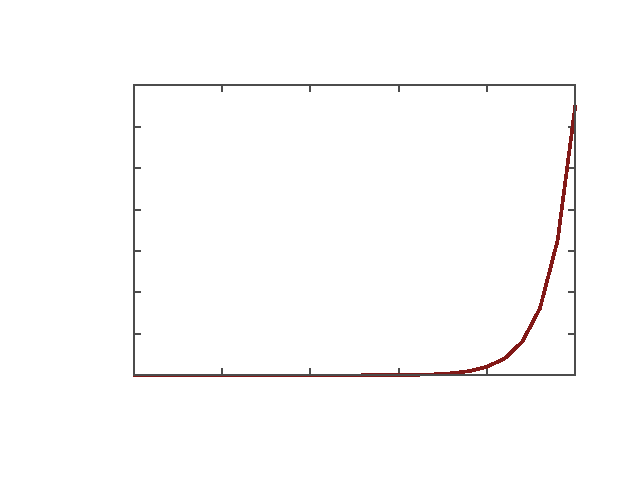
\includegraphics{./graficos/hanoi-linux-O0}}%
    \gplfronttext
  \end{picture}%
\endgroup

	\end{center}
\end{frame}

\begin{frame}{Datos de la eficiencia empírica}
	Hemos recopilado los datos de la eficiencia empírica de la ejecución de los distintos algoritmos en varias tablas comparativas. Los datos han sido obtenidos ejecutandose en la misma máquina con Linux y sin optimización.
	
	\vskip 0.5cm
	
	Hemos creado tablas para los distintos órdenes de eficiencia de los algoritmos y hemos puesto juntos aquellos que tienen el mismo.
	
	\vskip 0.5cm
	
	Finalmente, para cada tabla comparativa hemos creado una gráfica.
	
\end{frame}

%%% TABLAS ALGORITMOS O(n2) CON OPTIMIZACIÓN O0

\pgfplotstableread{datos/burbuja_datos/burbuja-linux-O0.dat}\burbujalinuxOCero
	\pgfplotstableread{datos/seleccion_datos/seleccion-linux-O0.dat}\seleccionlinuxOCero
	\pgfplotstableread{datos/insercion_datos/insercion-linux-O0.dat}\insercionlinuxOCero
	
	\pgfplotstablecreatecol[copy column from table={\burbujalinuxOCero}{[index] 1}] {Burbuja} {\burbujalinuxOCero}
	\pgfplotstablecreatecol[copy column from table={\seleccionlinuxOCero}{[index] 1}] {Selección} {\burbujalinuxOCero}
	\pgfplotstablecreatecol[copy column from table={\insercionlinuxOCero}{[index] 1}] {Inserción} {\burbujalinuxOCero}

\begin{frame}
	\begin{columns}[c] % align columns
		\begin{column}{.6\textwidth}
			\resizebox*{!}{9cm}{
				\pgfplotstabletypeset[columns={0, Burbuja, Inserción, Selección}]{\burbujalinuxOCero}
			}
		\end{column}%
		
		\hfill%
		
		\begin{column}{.3\textwidth}
			Algoritmos que son $O(n^2)$
		\end{column}%
		
	\end{columns}
\end{frame}

\begin{frame}
	\begin{center}
		% GNUPLOT: LaTeX picture with Postscript
\begingroup
  \makeatletter
  \providecommand\color[2][]{%
    \GenericError{(gnuplot) \space\space\space\@spaces}{%
      Package color not loaded in conjunction with
      terminal option `colourtext'%
    }{See the gnuplot documentation for explanation.%
    }{Either use 'blacktext' in gnuplot or load the package
      color.sty in LaTeX.}%
    \renewcommand\color[2][]{}%
  }%
  \providecommand\includegraphics[2][]{%
    \GenericError{(gnuplot) \space\space\space\@spaces}{%
      Package graphicx or graphics not loaded%
    }{See the gnuplot documentation for explanation.%
    }{The gnuplot epslatex terminal needs graphicx.sty or graphics.sty.}%
    \renewcommand\includegraphics[2][]{}%
  }%
  \providecommand\rotatebox[2]{#2}%
  \@ifundefined{ifGPcolor}{%
    \newif\ifGPcolor
    \GPcolortrue
  }{}%
  \@ifundefined{ifGPblacktext}{%
    \newif\ifGPblacktext
    \GPblacktextfalse
  }{}%
  % define a \g@addto@macro without @ in the name:
  \let\gplgaddtomacro\g@addto@macro
  % define empty templates for all commands taking text:
  \gdef\gplbacktext{}%
  \gdef\gplfronttext{}%
  \makeatother
  \ifGPblacktext
    % no textcolor at all
    \def\colorrgb#1{}%
    \def\colorgray#1{}%
  \else
    % gray or color?
    \ifGPcolor
      \def\colorrgb#1{\color[rgb]{#1}}%
      \def\colorgray#1{\color[gray]{#1}}%
      \expandafter\def\csname LTw\endcsname{\color{white}}%
      \expandafter\def\csname LTb\endcsname{\color{black}}%
      \expandafter\def\csname LTa\endcsname{\color{black}}%
      \expandafter\def\csname LT0\endcsname{\color[rgb]{1,0,0}}%
      \expandafter\def\csname LT1\endcsname{\color[rgb]{0,1,0}}%
      \expandafter\def\csname LT2\endcsname{\color[rgb]{0,0,1}}%
      \expandafter\def\csname LT3\endcsname{\color[rgb]{1,0,1}}%
      \expandafter\def\csname LT4\endcsname{\color[rgb]{0,1,1}}%
      \expandafter\def\csname LT5\endcsname{\color[rgb]{1,1,0}}%
      \expandafter\def\csname LT6\endcsname{\color[rgb]{0,0,0}}%
      \expandafter\def\csname LT7\endcsname{\color[rgb]{1,0.3,0}}%
      \expandafter\def\csname LT8\endcsname{\color[rgb]{0.5,0.5,0.5}}%
    \else
      % gray
      \def\colorrgb#1{\color{black}}%
      \def\colorgray#1{\color[gray]{#1}}%
      \expandafter\def\csname LTw\endcsname{\color{white}}%
      \expandafter\def\csname LTb\endcsname{\color{black}}%
      \expandafter\def\csname LTa\endcsname{\color{black}}%
      \expandafter\def\csname LT0\endcsname{\color{black}}%
      \expandafter\def\csname LT1\endcsname{\color{black}}%
      \expandafter\def\csname LT2\endcsname{\color{black}}%
      \expandafter\def\csname LT3\endcsname{\color{black}}%
      \expandafter\def\csname LT4\endcsname{\color{black}}%
      \expandafter\def\csname LT5\endcsname{\color{black}}%
      \expandafter\def\csname LT6\endcsname{\color{black}}%
      \expandafter\def\csname LT7\endcsname{\color{black}}%
      \expandafter\def\csname LT8\endcsname{\color{black}}%
    \fi
  \fi
    \setlength{\unitlength}{0.0500bp}%
    \ifx\gptboxheight\undefined%
      \newlength{\gptboxheight}%
      \newlength{\gptboxwidth}%
      \newsavebox{\gptboxtext}%
    \fi%
    \setlength{\fboxrule}{0.5pt}%
    \setlength{\fboxsep}{1pt}%
\begin{picture}(5760.00,4320.00)%
    \gplgaddtomacro\gplbacktext{%
      \colorrgb{0.30,0.30,0.30}%
      \put(990,1153){\makebox(0,0)[r]{\strut{}$\textcolor{text}{0}$}}%
      \colorrgb{0.30,0.30,0.30}%
      \put(990,1466){\makebox(0,0)[r]{\strut{}$\textcolor{text}{1}$}}%
      \colorrgb{0.30,0.30,0.30}%
      \put(990,1780){\makebox(0,0)[r]{\strut{}$\textcolor{text}{2}$}}%
      \colorrgb{0.30,0.30,0.30}%
      \put(990,2093){\makebox(0,0)[r]{\strut{}$\textcolor{text}{3}$}}%
      \colorrgb{0.30,0.30,0.30}%
      \put(990,2406){\makebox(0,0)[r]{\strut{}$\textcolor{text}{4}$}}%
      \colorrgb{0.30,0.30,0.30}%
      \put(990,2719){\makebox(0,0)[r]{\strut{}$\textcolor{text}{5}$}}%
      \colorrgb{0.30,0.30,0.30}%
      \put(990,3033){\makebox(0,0)[r]{\strut{}$\textcolor{text}{6}$}}%
      \colorrgb{0.30,0.30,0.30}%
      \put(990,3346){\makebox(0,0)[r]{\strut{}$\textcolor{text}{7}$}}%
      \colorrgb{0.30,0.30,0.30}%
      \put(990,3659){\makebox(0,0)[r]{\strut{}$\textcolor{text}{8}$}}%
      \colorrgb{0.30,0.30,0.30}%
      \put(1122,1021){\rotatebox{45}{\makebox(0,0)[r]{\strut{}$\textcolor{text}{0}$}}}%
      \colorrgb{0.30,0.30,0.30}%
      \put(1546,1021){\rotatebox{45}{\makebox(0,0)[r]{\strut{}$\textcolor{text}{5000}$}}}%
      \colorrgb{0.30,0.30,0.30}%
      \put(1970,1021){\rotatebox{45}{\makebox(0,0)[r]{\strut{}$\textcolor{text}{10000}$}}}%
      \colorrgb{0.30,0.30,0.30}%
      \put(2394,1021){\rotatebox{45}{\makebox(0,0)[r]{\strut{}$\textcolor{text}{15000}$}}}%
      \colorrgb{0.30,0.30,0.30}%
      \put(2818,1021){\rotatebox{45}{\makebox(0,0)[r]{\strut{}$\textcolor{text}{20000}$}}}%
      \colorrgb{0.30,0.30,0.30}%
      \put(3243,1021){\rotatebox{45}{\makebox(0,0)[r]{\strut{}$\textcolor{text}{25000}$}}}%
      \colorrgb{0.30,0.30,0.30}%
      \put(3667,1021){\rotatebox{45}{\makebox(0,0)[r]{\strut{}$\textcolor{text}{30000}$}}}%
      \colorrgb{0.30,0.30,0.30}%
      \put(4091,1021){\rotatebox{45}{\makebox(0,0)[r]{\strut{}$\textcolor{text}{35000}$}}}%
      \colorrgb{0.30,0.30,0.30}%
      \put(4515,1021){\rotatebox{45}{\makebox(0,0)[r]{\strut{}$\textcolor{text}{40000}$}}}%
      \colorrgb{0.30,0.30,0.30}%
      \put(4939,1021){\rotatebox{45}{\makebox(0,0)[r]{\strut{}$\textcolor{text}{45000}$}}}%
      \colorrgb{0.30,0.30,0.30}%
      \put(5363,1021){\rotatebox{45}{\makebox(0,0)[r]{\strut{}$\textcolor{text}{50000}$}}}%
    }%
    \gplgaddtomacro\gplfronttext{%
      \colorrgb{0.30,0.30,0.30}%
      \put(220,2406){\rotatebox{-270}{\makebox(0,0){\strut{}Tiempo de ejecución (s)}}}%
      \colorrgb{0.30,0.30,0.30}%
      \put(3242,220){\makebox(0,0){\strut{}Tamaño del vector (elementos)}}%
      \colorrgb{0.30,0.30,0.30}%
      \put(3242,3989){\makebox(0,0){\strut{}Algoritmos de ordenación $O(n^2)$}}%
      \csname LTb\endcsname%
      \put(4376,3486){\makebox(0,0)[r]{\strut{}Burbuja}}%
      \csname LTb\endcsname%
      \put(4376,3266){\makebox(0,0)[r]{\strut{}Inserción}}%
      \csname LTb\endcsname%
      \put(4376,3046){\makebox(0,0)[r]{\strut{}Selección}}%
    }%
    \gplbacktext
    \put(0,0){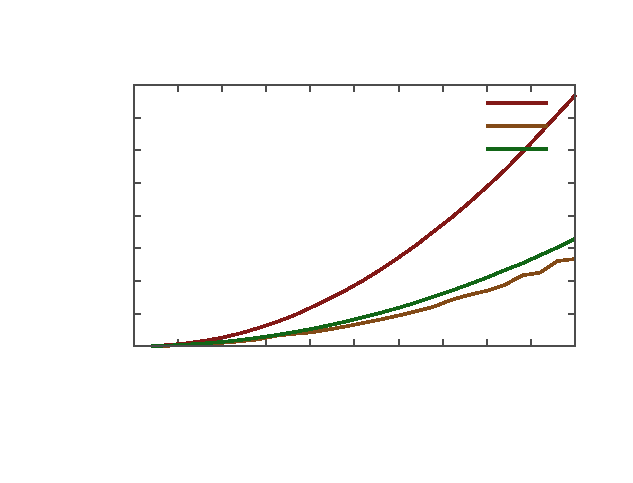
\includegraphics{./graficos/ncuadrado}}%
    \gplfronttext
  \end{picture}%
\endgroup

	\end{center}
\end{frame}

%%% TABLAS ALGORITMOS O(nlogn) CON OPTIMIZACIÓN O0

\pgfplotstableread{datos/mergesort_datos/mergesort-linux-O0.dat}\mergesortlinuxOCero
	\pgfplotstableread{datos/quicksort_datos/quicksort-linux-O0.dat}\quicksortlinuxOCero
	\pgfplotstableread{datos/heapsort_datos/heapsort-linux-O0.dat}\heapsortlinuxOCero
	
	\pgfplotstablecreatecol[copy column from table={\mergesortlinuxOCero}{[index] 1}] {Mergesort} {\mergesortlinuxOCero}
	\pgfplotstablecreatecol[copy column from table={\quicksortlinuxOCero}{[index] 1}] {Quicksort} {\mergesortlinuxOCero}
	\pgfplotstablecreatecol[copy column from table={\heapsortlinuxOCero}{[index] 1}] {Heapsort} {\mergesortlinuxOCero}

\begin{frame}
	\begin{columns}[c] % align columns
		\begin{column}{.6\textwidth}
			\resizebox*{!}{9cm}{
				\pgfplotstabletypeset[columns={0, Mergesort, Quicksort, Heapsort}]{\mergesortlinuxOCero}
			}
		\end{column}%
		
		\hfill%
		
		\begin{column}{.3\textwidth}
			Algoritmos que son $O(nlogn)$
		\end{column}%
		
	\end{columns}
\end{frame}

\begin{frame}
	\begin{center}
		\resizebox*{11cm}{!}{
				% GNUPLOT: LaTeX picture with Postscript
\begingroup
  \makeatletter
  \providecommand\color[2][]{%
    \GenericError{(gnuplot) \space\space\space\@spaces}{%
      Package color not loaded in conjunction with
      terminal option `colourtext'%
    }{See the gnuplot documentation for explanation.%
    }{Either use 'blacktext' in gnuplot or load the package
      color.sty in LaTeX.}%
    \renewcommand\color[2][]{}%
  }%
  \providecommand\includegraphics[2][]{%
    \GenericError{(gnuplot) \space\space\space\@spaces}{%
      Package graphicx or graphics not loaded%
    }{See the gnuplot documentation for explanation.%
    }{The gnuplot epslatex terminal needs graphicx.sty or graphics.sty.}%
    \renewcommand\includegraphics[2][]{}%
  }%
  \providecommand\rotatebox[2]{#2}%
  \@ifundefined{ifGPcolor}{%
    \newif\ifGPcolor
    \GPcolortrue
  }{}%
  \@ifundefined{ifGPblacktext}{%
    \newif\ifGPblacktext
    \GPblacktextfalse
  }{}%
  % define a \g@addto@macro without @ in the name:
  \let\gplgaddtomacro\g@addto@macro
  % define empty templates for all commands taking text:
  \gdef\gplbacktext{}%
  \gdef\gplfronttext{}%
  \makeatother
  \ifGPblacktext
    % no textcolor at all
    \def\colorrgb#1{}%
    \def\colorgray#1{}%
  \else
    % gray or color?
    \ifGPcolor
      \def\colorrgb#1{\color[rgb]{#1}}%
      \def\colorgray#1{\color[gray]{#1}}%
      \expandafter\def\csname LTw\endcsname{\color{white}}%
      \expandafter\def\csname LTb\endcsname{\color{black}}%
      \expandafter\def\csname LTa\endcsname{\color{black}}%
      \expandafter\def\csname LT0\endcsname{\color[rgb]{1,0,0}}%
      \expandafter\def\csname LT1\endcsname{\color[rgb]{0,1,0}}%
      \expandafter\def\csname LT2\endcsname{\color[rgb]{0,0,1}}%
      \expandafter\def\csname LT3\endcsname{\color[rgb]{1,0,1}}%
      \expandafter\def\csname LT4\endcsname{\color[rgb]{0,1,1}}%
      \expandafter\def\csname LT5\endcsname{\color[rgb]{1,1,0}}%
      \expandafter\def\csname LT6\endcsname{\color[rgb]{0,0,0}}%
      \expandafter\def\csname LT7\endcsname{\color[rgb]{1,0.3,0}}%
      \expandafter\def\csname LT8\endcsname{\color[rgb]{0.5,0.5,0.5}}%
    \else
      % gray
      \def\colorrgb#1{\color{black}}%
      \def\colorgray#1{\color[gray]{#1}}%
      \expandafter\def\csname LTw\endcsname{\color{white}}%
      \expandafter\def\csname LTb\endcsname{\color{black}}%
      \expandafter\def\csname LTa\endcsname{\color{black}}%
      \expandafter\def\csname LT0\endcsname{\color{black}}%
      \expandafter\def\csname LT1\endcsname{\color{black}}%
      \expandafter\def\csname LT2\endcsname{\color{black}}%
      \expandafter\def\csname LT3\endcsname{\color{black}}%
      \expandafter\def\csname LT4\endcsname{\color{black}}%
      \expandafter\def\csname LT5\endcsname{\color{black}}%
      \expandafter\def\csname LT6\endcsname{\color{black}}%
      \expandafter\def\csname LT7\endcsname{\color{black}}%
      \expandafter\def\csname LT8\endcsname{\color{black}}%
    \fi
  \fi
    \setlength{\unitlength}{0.0500bp}%
    \ifx\gptboxheight\undefined%
      \newlength{\gptboxheight}%
      \newlength{\gptboxwidth}%
      \newsavebox{\gptboxtext}%
    \fi%
    \setlength{\fboxrule}{0.5pt}%
    \setlength{\fboxsep}{1pt}%
\begin{picture}(5760.00,4320.00)%
    \gplgaddtomacro\gplbacktext{%
      \colorrgb{0.30,0.30,0.30}%
      \put(1650,1246){\makebox(0,0)[r]{\strut{}$\textcolor{text}{0.0001}$}}%
      \colorrgb{0.30,0.30,0.30}%
      \put(1650,2050){\makebox(0,0)[r]{\strut{}$\textcolor{text}{0.001}$}}%
      \colorrgb{0.30,0.30,0.30}%
      \put(1650,2855){\makebox(0,0)[r]{\strut{}$\textcolor{text}{0.01}$}}%
      \colorrgb{0.30,0.30,0.30}%
      \put(1650,3659){\makebox(0,0)[r]{\strut{}$\textcolor{text}{0.1}$}}%
      \colorrgb{0.30,0.30,0.30}%
      \put(1782,1114){\rotatebox{45}{\makebox(0,0)[r]{\strut{}$\textcolor{text}{0}$}}}%
      \colorrgb{0.30,0.30,0.30}%
      \put(2230,1114){\rotatebox{45}{\makebox(0,0)[r]{\strut{}$\textcolor{text}{20000}$}}}%
      \colorrgb{0.30,0.30,0.30}%
      \put(2677,1114){\rotatebox{45}{\makebox(0,0)[r]{\strut{}$\textcolor{text}{40000}$}}}%
      \colorrgb{0.30,0.30,0.30}%
      \put(3125,1114){\rotatebox{45}{\makebox(0,0)[r]{\strut{}$\textcolor{text}{60000}$}}}%
      \colorrgb{0.30,0.30,0.30}%
      \put(3573,1114){\rotatebox{45}{\makebox(0,0)[r]{\strut{}$\textcolor{text}{80000}$}}}%
      \colorrgb{0.30,0.30,0.30}%
      \put(4020,1114){\rotatebox{45}{\makebox(0,0)[r]{\strut{}$\textcolor{text}{100000}$}}}%
      \colorrgb{0.30,0.30,0.30}%
      \put(4468,1114){\rotatebox{45}{\makebox(0,0)[r]{\strut{}$\textcolor{text}{120000}$}}}%
      \colorrgb{0.30,0.30,0.30}%
      \put(4915,1114){\rotatebox{45}{\makebox(0,0)[r]{\strut{}$\textcolor{text}{140000}$}}}%
      \colorrgb{0.30,0.30,0.30}%
      \put(5363,1114){\rotatebox{45}{\makebox(0,0)[r]{\strut{}$\textcolor{text}{160000}$}}}%
    }%
    \gplgaddtomacro\gplfronttext{%
      \colorrgb{0.30,0.30,0.30}%
      \put(220,2452){\rotatebox{-270}{\makebox(0,0){\strut{}Tiempo de ejecución (s)}}}%
      \colorrgb{0.30,0.30,0.30}%
      \put(3572,220){\makebox(0,0){\strut{}Tamaño del vector (elementos)}}%
      \colorrgb{0.30,0.30,0.30}%
      \put(3572,3989){\makebox(0,0){\strut{}Algoritmos de ordenación $O(nlogn)$}}%
      \csname LTb\endcsname%
      \put(4376,3486){\makebox(0,0)[r]{\strut{}Mergesort}}%
      \csname LTb\endcsname%
      \put(4376,3266){\makebox(0,0)[r]{\strut{}Heapsort}}%
      \csname LTb\endcsname%
      \put(4376,3046){\makebox(0,0)[r]{\strut{}Quicksort}}%
    }%
    \gplbacktext
    \put(0,0){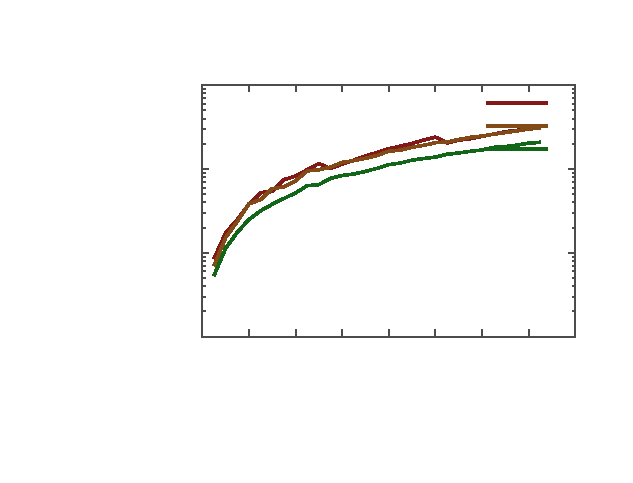
\includegraphics{./graficos/nlogn}}%
    \gplfronttext
  \end{picture}%
\endgroup

			}
	\end{center}
\end{frame}

%%% TABLA FLOYD
\begin{frame}
	\begin{columns}[c] % align columns
		\begin{column}{.6\textwidth}
			\resizebox*{!}{9cm}{
				\pgfplotstabletypeset[]{./datos/floyd_datos/floyd-linux-O0.dat}
			}
		\end{column}%
		
		\hfill%
		
		\begin{column}{.3\textwidth}
			Floyd
		\end{column}%
		
	\end{columns}
\end{frame}

%%% TABLA HANOI
\begin{frame}
	\begin{columns}[c] % align columns
		\begin{column}{.6\textwidth}
			\resizebox*{!}{9cm}{
				\pgfplotstabletypeset[]{./datos/hanoi_datos/hanoi-linux-O0.dat}
			}
		\end{column}%
		
		\hfill%
		
		\begin{column}{.3\textwidth}
			Hanoi
		\end{column}%
		
	\end{columns}
\end{frame}

\begin{frame}{Comparativa de los algoritmos de ordenación}
	Recopilando los datos de todos los algoritmos de ordenación hemos realizado una tabla comparativa en la que se muestra qué algoritmo es el más eficiente.
\end{frame}

\begin{frame}
	\begin{center}
		\resizebox*{11cm}{!}{
				% GNUPLOT: LaTeX picture with Postscript
\begingroup
  \makeatletter
  \providecommand\color[2][]{%
    \GenericError{(gnuplot) \space\space\space\@spaces}{%
      Package color not loaded in conjunction with
      terminal option `colourtext'%
    }{See the gnuplot documentation for explanation.%
    }{Either use 'blacktext' in gnuplot or load the package
      color.sty in LaTeX.}%
    \renewcommand\color[2][]{}%
  }%
  \providecommand\includegraphics[2][]{%
    \GenericError{(gnuplot) \space\space\space\@spaces}{%
      Package graphicx or graphics not loaded%
    }{See the gnuplot documentation for explanation.%
    }{The gnuplot epslatex terminal needs graphicx.sty or graphics.sty.}%
    \renewcommand\includegraphics[2][]{}%
  }%
  \providecommand\rotatebox[2]{#2}%
  \@ifundefined{ifGPcolor}{%
    \newif\ifGPcolor
    \GPcolortrue
  }{}%
  \@ifundefined{ifGPblacktext}{%
    \newif\ifGPblacktext
    \GPblacktextfalse
  }{}%
  % define a \g@addto@macro without @ in the name:
  \let\gplgaddtomacro\g@addto@macro
  % define empty templates for all commands taking text:
  \gdef\gplbacktext{}%
  \gdef\gplfronttext{}%
  \makeatother
  \ifGPblacktext
    % no textcolor at all
    \def\colorrgb#1{}%
    \def\colorgray#1{}%
  \else
    % gray or color?
    \ifGPcolor
      \def\colorrgb#1{\color[rgb]{#1}}%
      \def\colorgray#1{\color[gray]{#1}}%
      \expandafter\def\csname LTw\endcsname{\color{white}}%
      \expandafter\def\csname LTb\endcsname{\color{black}}%
      \expandafter\def\csname LTa\endcsname{\color{black}}%
      \expandafter\def\csname LT0\endcsname{\color[rgb]{1,0,0}}%
      \expandafter\def\csname LT1\endcsname{\color[rgb]{0,1,0}}%
      \expandafter\def\csname LT2\endcsname{\color[rgb]{0,0,1}}%
      \expandafter\def\csname LT3\endcsname{\color[rgb]{1,0,1}}%
      \expandafter\def\csname LT4\endcsname{\color[rgb]{0,1,1}}%
      \expandafter\def\csname LT5\endcsname{\color[rgb]{1,1,0}}%
      \expandafter\def\csname LT6\endcsname{\color[rgb]{0,0,0}}%
      \expandafter\def\csname LT7\endcsname{\color[rgb]{1,0.3,0}}%
      \expandafter\def\csname LT8\endcsname{\color[rgb]{0.5,0.5,0.5}}%
    \else
      % gray
      \def\colorrgb#1{\color{black}}%
      \def\colorgray#1{\color[gray]{#1}}%
      \expandafter\def\csname LTw\endcsname{\color{white}}%
      \expandafter\def\csname LTb\endcsname{\color{black}}%
      \expandafter\def\csname LTa\endcsname{\color{black}}%
      \expandafter\def\csname LT0\endcsname{\color{black}}%
      \expandafter\def\csname LT1\endcsname{\color{black}}%
      \expandafter\def\csname LT2\endcsname{\color{black}}%
      \expandafter\def\csname LT3\endcsname{\color{black}}%
      \expandafter\def\csname LT4\endcsname{\color{black}}%
      \expandafter\def\csname LT5\endcsname{\color{black}}%
      \expandafter\def\csname LT6\endcsname{\color{black}}%
      \expandafter\def\csname LT7\endcsname{\color{black}}%
      \expandafter\def\csname LT8\endcsname{\color{black}}%
    \fi
  \fi
    \setlength{\unitlength}{0.0500bp}%
    \ifx\gptboxheight\undefined%
      \newlength{\gptboxheight}%
      \newlength{\gptboxwidth}%
      \newsavebox{\gptboxtext}%
    \fi%
    \setlength{\fboxrule}{0.5pt}%
    \setlength{\fboxsep}{1pt}%
\begin{picture}(5760.00,4320.00)%
    \gplgaddtomacro\gplbacktext{%
      \colorrgb{0.30,0.30,0.30}%
      \put(1650,1246){\makebox(0,0)[r]{\strut{}$\textcolor{text}{0.0001}$}}%
      \colorrgb{0.30,0.30,0.30}%
      \put(1650,1648){\makebox(0,0)[r]{\strut{}$\textcolor{text}{0.001}$}}%
      \colorrgb{0.30,0.30,0.30}%
      \put(1650,2050){\makebox(0,0)[r]{\strut{}$\textcolor{text}{0.01}$}}%
      \colorrgb{0.30,0.30,0.30}%
      \put(1650,2453){\makebox(0,0)[r]{\strut{}$\textcolor{text}{0.1}$}}%
      \colorrgb{0.30,0.30,0.30}%
      \put(1650,2855){\makebox(0,0)[r]{\strut{}$\textcolor{text}{1}$}}%
      \colorrgb{0.30,0.30,0.30}%
      \put(1650,3257){\makebox(0,0)[r]{\strut{}$\textcolor{text}{10}$}}%
      \colorrgb{0.30,0.30,0.30}%
      \put(1650,3659){\makebox(0,0)[r]{\strut{}$\textcolor{text}{100}$}}%
      \colorrgb{0.30,0.30,0.30}%
      \put(1782,1114){\rotatebox{45}{\makebox(0,0)[r]{\strut{}$\textcolor{text}{0}$}}}%
      \colorrgb{0.30,0.30,0.30}%
      \put(2230,1114){\rotatebox{45}{\makebox(0,0)[r]{\strut{}$\textcolor{text}{20000}$}}}%
      \colorrgb{0.30,0.30,0.30}%
      \put(2677,1114){\rotatebox{45}{\makebox(0,0)[r]{\strut{}$\textcolor{text}{40000}$}}}%
      \colorrgb{0.30,0.30,0.30}%
      \put(3125,1114){\rotatebox{45}{\makebox(0,0)[r]{\strut{}$\textcolor{text}{60000}$}}}%
      \colorrgb{0.30,0.30,0.30}%
      \put(3573,1114){\rotatebox{45}{\makebox(0,0)[r]{\strut{}$\textcolor{text}{80000}$}}}%
      \colorrgb{0.30,0.30,0.30}%
      \put(4020,1114){\rotatebox{45}{\makebox(0,0)[r]{\strut{}$\textcolor{text}{100000}$}}}%
      \colorrgb{0.30,0.30,0.30}%
      \put(4468,1114){\rotatebox{45}{\makebox(0,0)[r]{\strut{}$\textcolor{text}{120000}$}}}%
      \colorrgb{0.30,0.30,0.30}%
      \put(4915,1114){\rotatebox{45}{\makebox(0,0)[r]{\strut{}$\textcolor{text}{140000}$}}}%
      \colorrgb{0.30,0.30,0.30}%
      \put(5363,1114){\rotatebox{45}{\makebox(0,0)[r]{\strut{}$\textcolor{text}{160000}$}}}%
    }%
    \gplgaddtomacro\gplfronttext{%
      \colorrgb{0.30,0.30,0.30}%
      \put(220,2452){\rotatebox{-270}{\makebox(0,0){\strut{}Tiempo de ejecución (s)}}}%
      \colorrgb{0.30,0.30,0.30}%
      \put(3572,220){\makebox(0,0){\strut{}Tamaño del vector (elementos)}}%
      \colorrgb{0.30,0.30,0.30}%
      \put(3572,3989){\makebox(0,0){\strut{}Algoritmos de ordenación}}%
      \csname LTb\endcsname%
      \put(4376,3486){\makebox(0,0)[r]{\strut{}Mergesort}}%
      \csname LTb\endcsname%
      \put(4376,3266){\makebox(0,0)[r]{\strut{}Heapsort}}%
      \csname LTb\endcsname%
      \put(4376,3046){\makebox(0,0)[r]{\strut{}Quicksort}}%
      \csname LTb\endcsname%
      \put(4376,2826){\makebox(0,0)[r]{\strut{}Burbuja}}%
      \csname LTb\endcsname%
      \put(4376,2606){\makebox(0,0)[r]{\strut{}Inserción}}%
      \csname LTb\endcsname%
      \put(4376,2386){\makebox(0,0)[r]{\strut{}Selección}}%
    }%
    \gplbacktext
    \put(0,0){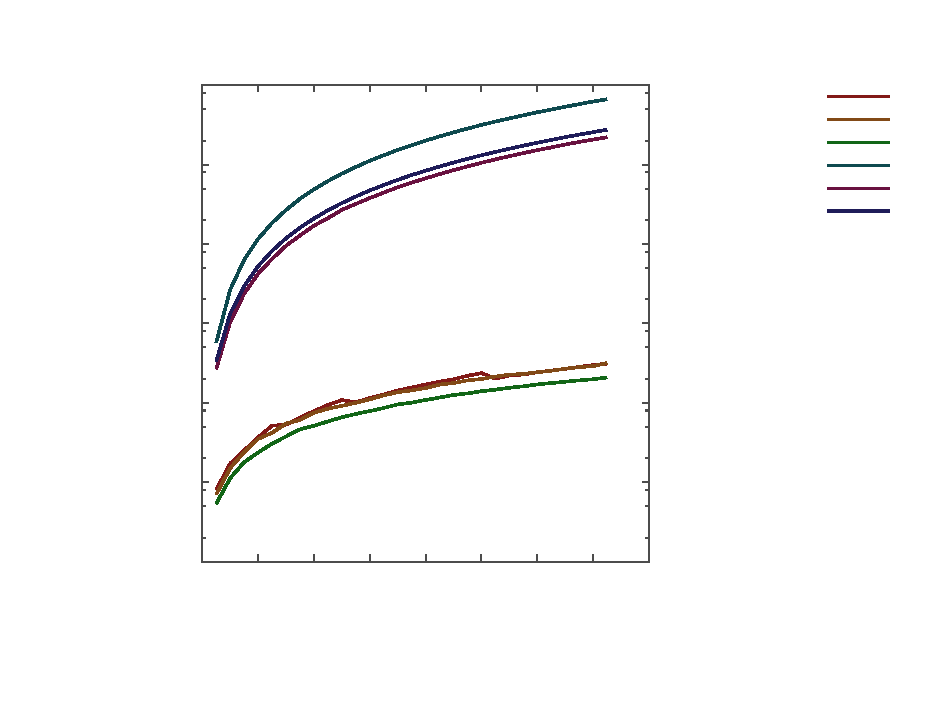
\includegraphics{./graficos/ordenacion}}%
    \gplfronttext
  \end{picture}%
\endgroup

			}
		
	\end{center}
\end{frame}


\begin{frame}
\frametitle{Comparativa según optimización y sistema operativo}

 Hemos elegido un representante de cada orden de eficiencia, y hemos realizado una comparativa para analizar cómo varían los tiempos de ejecución según el sistema operativo y el nivel de optimización.	
\end{frame}
	
\begin{frame}
\vspace{2em}
\textbf{Representante de $\boldsymbol{O(n^2)}$}
	\begin{center}
		% GNUPLOT: LaTeX picture with Postscript
\begingroup
  \makeatletter
  \providecommand\color[2][]{%
    \GenericError{(gnuplot) \space\space\space\@spaces}{%
      Package color not loaded in conjunction with
      terminal option `colourtext'%
    }{See the gnuplot documentation for explanation.%
    }{Either use 'blacktext' in gnuplot or load the package
      color.sty in LaTeX.}%
    \renewcommand\color[2][]{}%
  }%
  \providecommand\includegraphics[2][]{%
    \GenericError{(gnuplot) \space\space\space\@spaces}{%
      Package graphicx or graphics not loaded%
    }{See the gnuplot documentation for explanation.%
    }{The gnuplot epslatex terminal needs graphicx.sty or graphics.sty.}%
    \renewcommand\includegraphics[2][]{}%
  }%
  \providecommand\rotatebox[2]{#2}%
  \@ifundefined{ifGPcolor}{%
    \newif\ifGPcolor
    \GPcolortrue
  }{}%
  \@ifundefined{ifGPblacktext}{%
    \newif\ifGPblacktext
    \GPblacktextfalse
  }{}%
  % define a \g@addto@macro without @ in the name:
  \let\gplgaddtomacro\g@addto@macro
  % define empty templates for all commands taking text:
  \gdef\gplbacktext{}%
  \gdef\gplfronttext{}%
  \makeatother
  \ifGPblacktext
    % no textcolor at all
    \def\colorrgb#1{}%
    \def\colorgray#1{}%
  \else
    % gray or color?
    \ifGPcolor
      \def\colorrgb#1{\color[rgb]{#1}}%
      \def\colorgray#1{\color[gray]{#1}}%
      \expandafter\def\csname LTw\endcsname{\color{white}}%
      \expandafter\def\csname LTb\endcsname{\color{black}}%
      \expandafter\def\csname LTa\endcsname{\color{black}}%
      \expandafter\def\csname LT0\endcsname{\color[rgb]{1,0,0}}%
      \expandafter\def\csname LT1\endcsname{\color[rgb]{0,1,0}}%
      \expandafter\def\csname LT2\endcsname{\color[rgb]{0,0,1}}%
      \expandafter\def\csname LT3\endcsname{\color[rgb]{1,0,1}}%
      \expandafter\def\csname LT4\endcsname{\color[rgb]{0,1,1}}%
      \expandafter\def\csname LT5\endcsname{\color[rgb]{1,1,0}}%
      \expandafter\def\csname LT6\endcsname{\color[rgb]{0,0,0}}%
      \expandafter\def\csname LT7\endcsname{\color[rgb]{1,0.3,0}}%
      \expandafter\def\csname LT8\endcsname{\color[rgb]{0.5,0.5,0.5}}%
    \else
      % gray
      \def\colorrgb#1{\color{black}}%
      \def\colorgray#1{\color[gray]{#1}}%
      \expandafter\def\csname LTw\endcsname{\color{white}}%
      \expandafter\def\csname LTb\endcsname{\color{black}}%
      \expandafter\def\csname LTa\endcsname{\color{black}}%
      \expandafter\def\csname LT0\endcsname{\color{black}}%
      \expandafter\def\csname LT1\endcsname{\color{black}}%
      \expandafter\def\csname LT2\endcsname{\color{black}}%
      \expandafter\def\csname LT3\endcsname{\color{black}}%
      \expandafter\def\csname LT4\endcsname{\color{black}}%
      \expandafter\def\csname LT5\endcsname{\color{black}}%
      \expandafter\def\csname LT6\endcsname{\color{black}}%
      \expandafter\def\csname LT7\endcsname{\color{black}}%
      \expandafter\def\csname LT8\endcsname{\color{black}}%
    \fi
  \fi
    \setlength{\unitlength}{0.0500bp}%
    \ifx\gptboxheight\undefined%
      \newlength{\gptboxheight}%
      \newlength{\gptboxwidth}%
      \newsavebox{\gptboxtext}%
    \fi%
    \setlength{\fboxrule}{0.5pt}%
    \setlength{\fboxsep}{1pt}%
\begin{picture}(5760.00,4320.00)%
    \gplgaddtomacro\gplbacktext{%
      \colorrgb{0.30,0.30,0.30}%
      \put(1254,1153){\makebox(0,0)[r]{\strut{}$\textcolor{text}{0}$}}%
      \colorrgb{0.30,0.30,0.30}%
      \put(1254,1571){\makebox(0,0)[r]{\strut{}$\textcolor{text}{0.5}$}}%
      \colorrgb{0.30,0.30,0.30}%
      \put(1254,1988){\makebox(0,0)[r]{\strut{}$\textcolor{text}{1}$}}%
      \colorrgb{0.30,0.30,0.30}%
      \put(1254,2406){\makebox(0,0)[r]{\strut{}$\textcolor{text}{1.5}$}}%
      \colorrgb{0.30,0.30,0.30}%
      \put(1254,2824){\makebox(0,0)[r]{\strut{}$\textcolor{text}{2}$}}%
      \colorrgb{0.30,0.30,0.30}%
      \put(1254,3241){\makebox(0,0)[r]{\strut{}$\textcolor{text}{2.5}$}}%
      \colorrgb{0.30,0.30,0.30}%
      \put(1254,3659){\makebox(0,0)[r]{\strut{}$\textcolor{text}{3}$}}%
      \colorrgb{0.30,0.30,0.30}%
      \put(1386,1021){\rotatebox{45}{\makebox(0,0)[r]{\strut{}$\textcolor{text}{0}$}}}%
      \colorrgb{0.30,0.30,0.30}%
      \put(1784,1021){\rotatebox{45}{\makebox(0,0)[r]{\strut{}$\textcolor{text}{5000}$}}}%
      \colorrgb{0.30,0.30,0.30}%
      \put(2181,1021){\rotatebox{45}{\makebox(0,0)[r]{\strut{}$\textcolor{text}{10000}$}}}%
      \colorrgb{0.30,0.30,0.30}%
      \put(2579,1021){\rotatebox{45}{\makebox(0,0)[r]{\strut{}$\textcolor{text}{15000}$}}}%
      \colorrgb{0.30,0.30,0.30}%
      \put(2977,1021){\rotatebox{45}{\makebox(0,0)[r]{\strut{}$\textcolor{text}{20000}$}}}%
      \colorrgb{0.30,0.30,0.30}%
      \put(3375,1021){\rotatebox{45}{\makebox(0,0)[r]{\strut{}$\textcolor{text}{25000}$}}}%
      \colorrgb{0.30,0.30,0.30}%
      \put(3772,1021){\rotatebox{45}{\makebox(0,0)[r]{\strut{}$\textcolor{text}{30000}$}}}%
      \colorrgb{0.30,0.30,0.30}%
      \put(4170,1021){\rotatebox{45}{\makebox(0,0)[r]{\strut{}$\textcolor{text}{35000}$}}}%
      \colorrgb{0.30,0.30,0.30}%
      \put(4568,1021){\rotatebox{45}{\makebox(0,0)[r]{\strut{}$\textcolor{text}{40000}$}}}%
      \colorrgb{0.30,0.30,0.30}%
      \put(4965,1021){\rotatebox{45}{\makebox(0,0)[r]{\strut{}$\textcolor{text}{45000}$}}}%
      \colorrgb{0.30,0.30,0.30}%
      \put(5363,1021){\rotatebox{45}{\makebox(0,0)[r]{\strut{}$\textcolor{text}{50000}$}}}%
    }%
    \gplgaddtomacro\gplfronttext{%
      \colorrgb{0.30,0.30,0.30}%
      \put(220,2406){\rotatebox{-270}{\makebox(0,0){\strut{}Tiempo de ejecución (s)}}}%
      \colorrgb{0.30,0.30,0.30}%
      \put(3374,220){\makebox(0,0){\strut{}Tamaño del vector (elementos)}}%
      \colorrgb{0.30,0.30,0.30}%
      \put(3374,3989){\makebox(0,0){\strut{}Comparación inserción en macOS y Linux}}%
      \csname LTb\endcsname%
      \put(4376,3486){\makebox(0,0)[r]{\strut{}Linux}}%
      \csname LTb\endcsname%
      \put(4376,3266){\makebox(0,0)[r]{\strut{}Mac}}%
    }%
    \gplbacktext
    \put(0,0){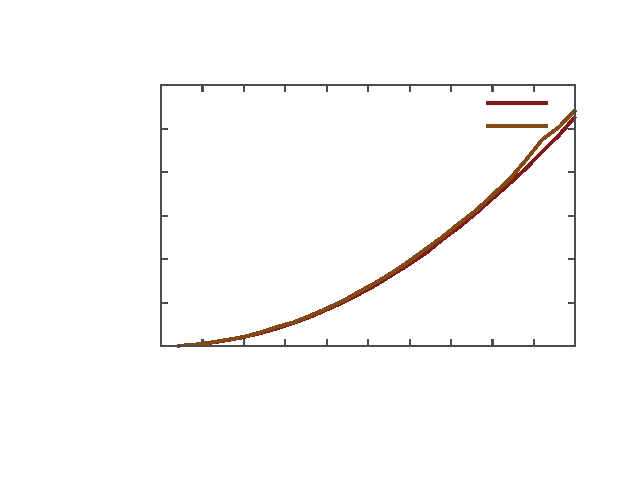
\includegraphics{./graficos/insercion-maclinux}}%
    \gplfronttext
  \end{picture}%
\endgroup

	\end{center}
\end{frame}

\begin{frame}
\vspace{2em}
\textbf{Representante de $\boldsymbol{O(n^2)}$}
	\begin{center}
		% GNUPLOT: LaTeX picture with Postscript
\begingroup
  \makeatletter
  \providecommand\color[2][]{%
    \GenericError{(gnuplot) \space\space\space\@spaces}{%
      Package color not loaded in conjunction with
      terminal option `colourtext'%
    }{See the gnuplot documentation for explanation.%
    }{Either use 'blacktext' in gnuplot or load the package
      color.sty in LaTeX.}%
    \renewcommand\color[2][]{}%
  }%
  \providecommand\includegraphics[2][]{%
    \GenericError{(gnuplot) \space\space\space\@spaces}{%
      Package graphicx or graphics not loaded%
    }{See the gnuplot documentation for explanation.%
    }{The gnuplot epslatex terminal needs graphicx.sty or graphics.sty.}%
    \renewcommand\includegraphics[2][]{}%
  }%
  \providecommand\rotatebox[2]{#2}%
  \@ifundefined{ifGPcolor}{%
    \newif\ifGPcolor
    \GPcolortrue
  }{}%
  \@ifundefined{ifGPblacktext}{%
    \newif\ifGPblacktext
    \GPblacktextfalse
  }{}%
  % define a \g@addto@macro without @ in the name:
  \let\gplgaddtomacro\g@addto@macro
  % define empty templates for all commands taking text:
  \gdef\gplbacktext{}%
  \gdef\gplfronttext{}%
  \makeatother
  \ifGPblacktext
    % no textcolor at all
    \def\colorrgb#1{}%
    \def\colorgray#1{}%
  \else
    % gray or color?
    \ifGPcolor
      \def\colorrgb#1{\color[rgb]{#1}}%
      \def\colorgray#1{\color[gray]{#1}}%
      \expandafter\def\csname LTw\endcsname{\color{white}}%
      \expandafter\def\csname LTb\endcsname{\color{black}}%
      \expandafter\def\csname LTa\endcsname{\color{black}}%
      \expandafter\def\csname LT0\endcsname{\color[rgb]{1,0,0}}%
      \expandafter\def\csname LT1\endcsname{\color[rgb]{0,1,0}}%
      \expandafter\def\csname LT2\endcsname{\color[rgb]{0,0,1}}%
      \expandafter\def\csname LT3\endcsname{\color[rgb]{1,0,1}}%
      \expandafter\def\csname LT4\endcsname{\color[rgb]{0,1,1}}%
      \expandafter\def\csname LT5\endcsname{\color[rgb]{1,1,0}}%
      \expandafter\def\csname LT6\endcsname{\color[rgb]{0,0,0}}%
      \expandafter\def\csname LT7\endcsname{\color[rgb]{1,0.3,0}}%
      \expandafter\def\csname LT8\endcsname{\color[rgb]{0.5,0.5,0.5}}%
    \else
      % gray
      \def\colorrgb#1{\color{black}}%
      \def\colorgray#1{\color[gray]{#1}}%
      \expandafter\def\csname LTw\endcsname{\color{white}}%
      \expandafter\def\csname LTb\endcsname{\color{black}}%
      \expandafter\def\csname LTa\endcsname{\color{black}}%
      \expandafter\def\csname LT0\endcsname{\color{black}}%
      \expandafter\def\csname LT1\endcsname{\color{black}}%
      \expandafter\def\csname LT2\endcsname{\color{black}}%
      \expandafter\def\csname LT3\endcsname{\color{black}}%
      \expandafter\def\csname LT4\endcsname{\color{black}}%
      \expandafter\def\csname LT5\endcsname{\color{black}}%
      \expandafter\def\csname LT6\endcsname{\color{black}}%
      \expandafter\def\csname LT7\endcsname{\color{black}}%
      \expandafter\def\csname LT8\endcsname{\color{black}}%
    \fi
  \fi
    \setlength{\unitlength}{0.0500bp}%
    \ifx\gptboxheight\undefined%
      \newlength{\gptboxheight}%
      \newlength{\gptboxwidth}%
      \newsavebox{\gptboxtext}%
    \fi%
    \setlength{\fboxrule}{0.5pt}%
    \setlength{\fboxsep}{1pt}%
\begin{picture}(5760.00,4320.00)%
    \gplgaddtomacro\gplbacktext{%
      \colorrgb{0.30,0.30,0.30}%
      \put(1254,1153){\makebox(0,0)[r]{\strut{}$\textcolor{text}{0}$}}%
      \colorrgb{0.30,0.30,0.30}%
      \put(1254,1571){\makebox(0,0)[r]{\strut{}$\textcolor{text}{0.5}$}}%
      \colorrgb{0.30,0.30,0.30}%
      \put(1254,1988){\makebox(0,0)[r]{\strut{}$\textcolor{text}{1}$}}%
      \colorrgb{0.30,0.30,0.30}%
      \put(1254,2406){\makebox(0,0)[r]{\strut{}$\textcolor{text}{1.5}$}}%
      \colorrgb{0.30,0.30,0.30}%
      \put(1254,2824){\makebox(0,0)[r]{\strut{}$\textcolor{text}{2}$}}%
      \colorrgb{0.30,0.30,0.30}%
      \put(1254,3241){\makebox(0,0)[r]{\strut{}$\textcolor{text}{2.5}$}}%
      \colorrgb{0.30,0.30,0.30}%
      \put(1254,3659){\makebox(0,0)[r]{\strut{}$\textcolor{text}{3}$}}%
      \colorrgb{0.30,0.30,0.30}%
      \put(1386,1021){\rotatebox{45}{\makebox(0,0)[r]{\strut{}$\textcolor{text}{0}$}}}%
      \colorrgb{0.30,0.30,0.30}%
      \put(1784,1021){\rotatebox{45}{\makebox(0,0)[r]{\strut{}$\textcolor{text}{5000}$}}}%
      \colorrgb{0.30,0.30,0.30}%
      \put(2181,1021){\rotatebox{45}{\makebox(0,0)[r]{\strut{}$\textcolor{text}{10000}$}}}%
      \colorrgb{0.30,0.30,0.30}%
      \put(2579,1021){\rotatebox{45}{\makebox(0,0)[r]{\strut{}$\textcolor{text}{15000}$}}}%
      \colorrgb{0.30,0.30,0.30}%
      \put(2977,1021){\rotatebox{45}{\makebox(0,0)[r]{\strut{}$\textcolor{text}{20000}$}}}%
      \colorrgb{0.30,0.30,0.30}%
      \put(3375,1021){\rotatebox{45}{\makebox(0,0)[r]{\strut{}$\textcolor{text}{25000}$}}}%
      \colorrgb{0.30,0.30,0.30}%
      \put(3772,1021){\rotatebox{45}{\makebox(0,0)[r]{\strut{}$\textcolor{text}{30000}$}}}%
      \colorrgb{0.30,0.30,0.30}%
      \put(4170,1021){\rotatebox{45}{\makebox(0,0)[r]{\strut{}$\textcolor{text}{35000}$}}}%
      \colorrgb{0.30,0.30,0.30}%
      \put(4568,1021){\rotatebox{45}{\makebox(0,0)[r]{\strut{}$\textcolor{text}{40000}$}}}%
      \colorrgb{0.30,0.30,0.30}%
      \put(4965,1021){\rotatebox{45}{\makebox(0,0)[r]{\strut{}$\textcolor{text}{45000}$}}}%
      \colorrgb{0.30,0.30,0.30}%
      \put(5363,1021){\rotatebox{45}{\makebox(0,0)[r]{\strut{}$\textcolor{text}{50000}$}}}%
    }%
    \gplgaddtomacro\gplfronttext{%
      \colorrgb{0.30,0.30,0.30}%
      \put(220,2406){\rotatebox{-270}{\makebox(0,0){\strut{}Tiempo de ejecución (s)}}}%
      \colorrgb{0.30,0.30,0.30}%
      \put(3374,220){\makebox(0,0){\strut{}Tamaño del vector (elementos)}}%
      \colorrgb{0.30,0.30,0.30}%
      \put(3374,3989){\makebox(0,0){\strut{}Comparación inserción en Linux con distinta optimización}}%
      \csname LTb\endcsname%
      \put(4376,3486){\makebox(0,0)[r]{\strut{}O0}}%
      \csname LTb\endcsname%
      \put(4376,3266){\makebox(0,0)[r]{\strut{}O1}}%
      \csname LTb\endcsname%
      \put(4376,3046){\makebox(0,0)[r]{\strut{}O2}}%
      \csname LTb\endcsname%
      \put(4376,2826){\makebox(0,0)[r]{\strut{}O3}}%
    }%
    \gplbacktext
    \put(0,0){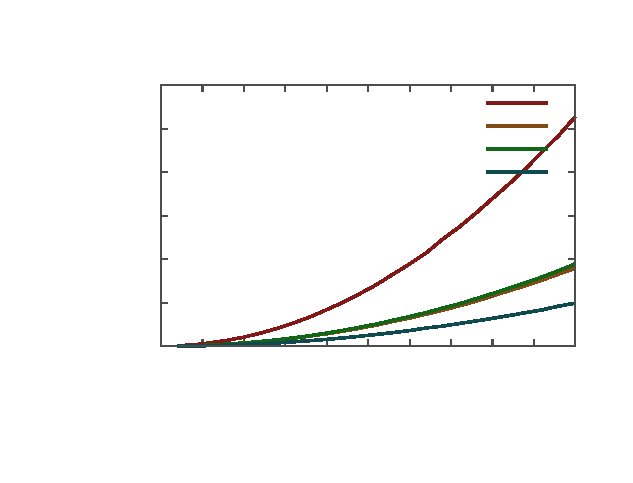
\includegraphics{./graficos/insercion-linux-opt}}%
    \gplfronttext
  \end{picture}%
\endgroup

	\end{center}
\end{frame}

\begin{frame}
\vspace{2em}
\textbf{Representante de $\boldsymbol{O(n\log n)}$}
	\begin{center}
		% GNUPLOT: LaTeX picture with Postscript
\begingroup
  \makeatletter
  \providecommand\color[2][]{%
    \GenericError{(gnuplot) \space\space\space\@spaces}{%
      Package color not loaded in conjunction with
      terminal option `colourtext'%
    }{See the gnuplot documentation for explanation.%
    }{Either use 'blacktext' in gnuplot or load the package
      color.sty in LaTeX.}%
    \renewcommand\color[2][]{}%
  }%
  \providecommand\includegraphics[2][]{%
    \GenericError{(gnuplot) \space\space\space\@spaces}{%
      Package graphicx or graphics not loaded%
    }{See the gnuplot documentation for explanation.%
    }{The gnuplot epslatex terminal needs graphicx.sty or graphics.sty.}%
    \renewcommand\includegraphics[2][]{}%
  }%
  \providecommand\rotatebox[2]{#2}%
  \@ifundefined{ifGPcolor}{%
    \newif\ifGPcolor
    \GPcolortrue
  }{}%
  \@ifundefined{ifGPblacktext}{%
    \newif\ifGPblacktext
    \GPblacktextfalse
  }{}%
  % define a \g@addto@macro without @ in the name:
  \let\gplgaddtomacro\g@addto@macro
  % define empty templates for all commands taking text:
  \gdef\gplbacktext{}%
  \gdef\gplfronttext{}%
  \makeatother
  \ifGPblacktext
    % no textcolor at all
    \def\colorrgb#1{}%
    \def\colorgray#1{}%
  \else
    % gray or color?
    \ifGPcolor
      \def\colorrgb#1{\color[rgb]{#1}}%
      \def\colorgray#1{\color[gray]{#1}}%
      \expandafter\def\csname LTw\endcsname{\color{white}}%
      \expandafter\def\csname LTb\endcsname{\color{black}}%
      \expandafter\def\csname LTa\endcsname{\color{black}}%
      \expandafter\def\csname LT0\endcsname{\color[rgb]{1,0,0}}%
      \expandafter\def\csname LT1\endcsname{\color[rgb]{0,1,0}}%
      \expandafter\def\csname LT2\endcsname{\color[rgb]{0,0,1}}%
      \expandafter\def\csname LT3\endcsname{\color[rgb]{1,0,1}}%
      \expandafter\def\csname LT4\endcsname{\color[rgb]{0,1,1}}%
      \expandafter\def\csname LT5\endcsname{\color[rgb]{1,1,0}}%
      \expandafter\def\csname LT6\endcsname{\color[rgb]{0,0,0}}%
      \expandafter\def\csname LT7\endcsname{\color[rgb]{1,0.3,0}}%
      \expandafter\def\csname LT8\endcsname{\color[rgb]{0.5,0.5,0.5}}%
    \else
      % gray
      \def\colorrgb#1{\color{black}}%
      \def\colorgray#1{\color[gray]{#1}}%
      \expandafter\def\csname LTw\endcsname{\color{white}}%
      \expandafter\def\csname LTb\endcsname{\color{black}}%
      \expandafter\def\csname LTa\endcsname{\color{black}}%
      \expandafter\def\csname LT0\endcsname{\color{black}}%
      \expandafter\def\csname LT1\endcsname{\color{black}}%
      \expandafter\def\csname LT2\endcsname{\color{black}}%
      \expandafter\def\csname LT3\endcsname{\color{black}}%
      \expandafter\def\csname LT4\endcsname{\color{black}}%
      \expandafter\def\csname LT5\endcsname{\color{black}}%
      \expandafter\def\csname LT6\endcsname{\color{black}}%
      \expandafter\def\csname LT7\endcsname{\color{black}}%
      \expandafter\def\csname LT8\endcsname{\color{black}}%
    \fi
  \fi
    \setlength{\unitlength}{0.0500bp}%
    \ifx\gptboxheight\undefined%
      \newlength{\gptboxheight}%
      \newlength{\gptboxwidth}%
      \newsavebox{\gptboxtext}%
    \fi%
    \setlength{\fboxrule}{0.5pt}%
    \setlength{\fboxsep}{1pt}%
\begin{picture}(5760.00,4320.00)%
    \gplgaddtomacro\gplbacktext{%
      \colorrgb{0.30,0.30,0.30}%
      \put(1518,1246){\makebox(0,0)[r]{\strut{}$\textcolor{text}{0}$}}%
      \colorrgb{0.30,0.30,0.30}%
      \put(1518,1729){\makebox(0,0)[r]{\strut{}$\textcolor{text}{0.005}$}}%
      \colorrgb{0.30,0.30,0.30}%
      \put(1518,2211){\makebox(0,0)[r]{\strut{}$\textcolor{text}{0.01}$}}%
      \colorrgb{0.30,0.30,0.30}%
      \put(1518,2694){\makebox(0,0)[r]{\strut{}$\textcolor{text}{0.015}$}}%
      \colorrgb{0.30,0.30,0.30}%
      \put(1518,3176){\makebox(0,0)[r]{\strut{}$\textcolor{text}{0.02}$}}%
      \colorrgb{0.30,0.30,0.30}%
      \put(1518,3659){\makebox(0,0)[r]{\strut{}$\textcolor{text}{0.025}$}}%
      \colorrgb{0.30,0.30,0.30}%
      \put(1650,1114){\rotatebox{45}{\makebox(0,0)[r]{\strut{}$\textcolor{text}{0}$}}}%
      \colorrgb{0.30,0.30,0.30}%
      \put(2114,1114){\rotatebox{45}{\makebox(0,0)[r]{\strut{}$\textcolor{text}{20000}$}}}%
      \colorrgb{0.30,0.30,0.30}%
      \put(2578,1114){\rotatebox{45}{\makebox(0,0)[r]{\strut{}$\textcolor{text}{40000}$}}}%
      \colorrgb{0.30,0.30,0.30}%
      \put(3042,1114){\rotatebox{45}{\makebox(0,0)[r]{\strut{}$\textcolor{text}{60000}$}}}%
      \colorrgb{0.30,0.30,0.30}%
      \put(3507,1114){\rotatebox{45}{\makebox(0,0)[r]{\strut{}$\textcolor{text}{80000}$}}}%
      \colorrgb{0.30,0.30,0.30}%
      \put(3971,1114){\rotatebox{45}{\makebox(0,0)[r]{\strut{}$\textcolor{text}{100000}$}}}%
      \colorrgb{0.30,0.30,0.30}%
      \put(4435,1114){\rotatebox{45}{\makebox(0,0)[r]{\strut{}$\textcolor{text}{120000}$}}}%
      \colorrgb{0.30,0.30,0.30}%
      \put(4899,1114){\rotatebox{45}{\makebox(0,0)[r]{\strut{}$\textcolor{text}{140000}$}}}%
      \colorrgb{0.30,0.30,0.30}%
      \put(5363,1114){\rotatebox{45}{\makebox(0,0)[r]{\strut{}$\textcolor{text}{160000}$}}}%
    }%
    \gplgaddtomacro\gplfronttext{%
      \colorrgb{0.30,0.30,0.30}%
      \put(220,2452){\rotatebox{-270}{\makebox(0,0){\strut{}Tiempo de ejecución (s)}}}%
      \colorrgb{0.30,0.30,0.30}%
      \put(3506,220){\makebox(0,0){\strut{}Tamaño del vector (elementos)}}%
      \colorrgb{0.30,0.30,0.30}%
      \put(3506,3989){\makebox(0,0){\strut{}Comparación quicksort en macOS y Linux}}%
      \csname LTb\endcsname%
      \put(4376,3486){\makebox(0,0)[r]{\strut{}Linux}}%
      \csname LTb\endcsname%
      \put(4376,3266){\makebox(0,0)[r]{\strut{}Mac}}%
    }%
    \gplbacktext
    \put(0,0){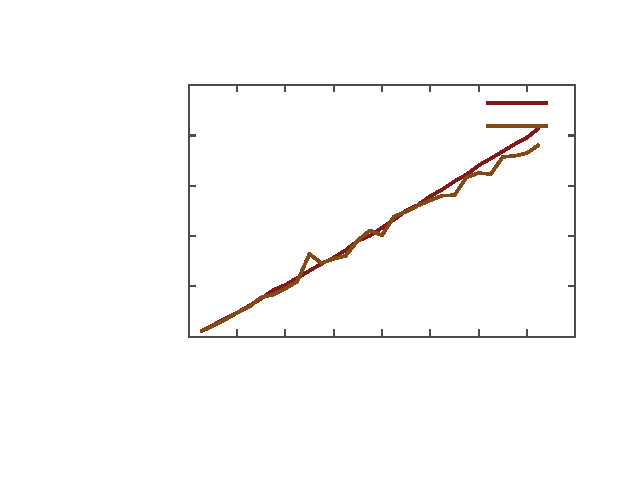
\includegraphics{./graficos/quicksort-maclinux}}%
    \gplfronttext
  \end{picture}%
\endgroup

	\end{center}
\end{frame}

\begin{frame}
\vspace{2em}
\textbf{Representante de $\boldsymbol{O(n\log n)}$}
	\begin{center}
		% GNUPLOT: LaTeX picture with Postscript
\begingroup
  \makeatletter
  \providecommand\color[2][]{%
    \GenericError{(gnuplot) \space\space\space\@spaces}{%
      Package color not loaded in conjunction with
      terminal option `colourtext'%
    }{See the gnuplot documentation for explanation.%
    }{Either use 'blacktext' in gnuplot or load the package
      color.sty in LaTeX.}%
    \renewcommand\color[2][]{}%
  }%
  \providecommand\includegraphics[2][]{%
    \GenericError{(gnuplot) \space\space\space\@spaces}{%
      Package graphicx or graphics not loaded%
    }{See the gnuplot documentation for explanation.%
    }{The gnuplot epslatex terminal needs graphicx.sty or graphics.sty.}%
    \renewcommand\includegraphics[2][]{}%
  }%
  \providecommand\rotatebox[2]{#2}%
  \@ifundefined{ifGPcolor}{%
    \newif\ifGPcolor
    \GPcolortrue
  }{}%
  \@ifundefined{ifGPblacktext}{%
    \newif\ifGPblacktext
    \GPblacktextfalse
  }{}%
  % define a \g@addto@macro without @ in the name:
  \let\gplgaddtomacro\g@addto@macro
  % define empty templates for all commands taking text:
  \gdef\gplbacktext{}%
  \gdef\gplfronttext{}%
  \makeatother
  \ifGPblacktext
    % no textcolor at all
    \def\colorrgb#1{}%
    \def\colorgray#1{}%
  \else
    % gray or color?
    \ifGPcolor
      \def\colorrgb#1{\color[rgb]{#1}}%
      \def\colorgray#1{\color[gray]{#1}}%
      \expandafter\def\csname LTw\endcsname{\color{white}}%
      \expandafter\def\csname LTb\endcsname{\color{black}}%
      \expandafter\def\csname LTa\endcsname{\color{black}}%
      \expandafter\def\csname LT0\endcsname{\color[rgb]{1,0,0}}%
      \expandafter\def\csname LT1\endcsname{\color[rgb]{0,1,0}}%
      \expandafter\def\csname LT2\endcsname{\color[rgb]{0,0,1}}%
      \expandafter\def\csname LT3\endcsname{\color[rgb]{1,0,1}}%
      \expandafter\def\csname LT4\endcsname{\color[rgb]{0,1,1}}%
      \expandafter\def\csname LT5\endcsname{\color[rgb]{1,1,0}}%
      \expandafter\def\csname LT6\endcsname{\color[rgb]{0,0,0}}%
      \expandafter\def\csname LT7\endcsname{\color[rgb]{1,0.3,0}}%
      \expandafter\def\csname LT8\endcsname{\color[rgb]{0.5,0.5,0.5}}%
    \else
      % gray
      \def\colorrgb#1{\color{black}}%
      \def\colorgray#1{\color[gray]{#1}}%
      \expandafter\def\csname LTw\endcsname{\color{white}}%
      \expandafter\def\csname LTb\endcsname{\color{black}}%
      \expandafter\def\csname LTa\endcsname{\color{black}}%
      \expandafter\def\csname LT0\endcsname{\color{black}}%
      \expandafter\def\csname LT1\endcsname{\color{black}}%
      \expandafter\def\csname LT2\endcsname{\color{black}}%
      \expandafter\def\csname LT3\endcsname{\color{black}}%
      \expandafter\def\csname LT4\endcsname{\color{black}}%
      \expandafter\def\csname LT5\endcsname{\color{black}}%
      \expandafter\def\csname LT6\endcsname{\color{black}}%
      \expandafter\def\csname LT7\endcsname{\color{black}}%
      \expandafter\def\csname LT8\endcsname{\color{black}}%
    \fi
  \fi
    \setlength{\unitlength}{0.0500bp}%
    \ifx\gptboxheight\undefined%
      \newlength{\gptboxheight}%
      \newlength{\gptboxwidth}%
      \newsavebox{\gptboxtext}%
    \fi%
    \setlength{\fboxrule}{0.5pt}%
    \setlength{\fboxsep}{1pt}%
\begin{picture}(5760.00,4320.00)%
    \gplgaddtomacro\gplbacktext{%
      \colorrgb{0.30,0.30,0.30}%
      \put(1518,1246){\makebox(0,0)[r]{\strut{}$\textcolor{text}{0}$}}%
      \colorrgb{0.30,0.30,0.30}%
      \put(1518,1729){\makebox(0,0)[r]{\strut{}$\textcolor{text}{0.005}$}}%
      \colorrgb{0.30,0.30,0.30}%
      \put(1518,2211){\makebox(0,0)[r]{\strut{}$\textcolor{text}{0.01}$}}%
      \colorrgb{0.30,0.30,0.30}%
      \put(1518,2694){\makebox(0,0)[r]{\strut{}$\textcolor{text}{0.015}$}}%
      \colorrgb{0.30,0.30,0.30}%
      \put(1518,3176){\makebox(0,0)[r]{\strut{}$\textcolor{text}{0.02}$}}%
      \colorrgb{0.30,0.30,0.30}%
      \put(1518,3659){\makebox(0,0)[r]{\strut{}$\textcolor{text}{0.025}$}}%
      \colorrgb{0.30,0.30,0.30}%
      \put(1650,1114){\rotatebox{45}{\makebox(0,0)[r]{\strut{}$\textcolor{text}{0}$}}}%
      \colorrgb{0.30,0.30,0.30}%
      \put(2114,1114){\rotatebox{45}{\makebox(0,0)[r]{\strut{}$\textcolor{text}{20000}$}}}%
      \colorrgb{0.30,0.30,0.30}%
      \put(2578,1114){\rotatebox{45}{\makebox(0,0)[r]{\strut{}$\textcolor{text}{40000}$}}}%
      \colorrgb{0.30,0.30,0.30}%
      \put(3042,1114){\rotatebox{45}{\makebox(0,0)[r]{\strut{}$\textcolor{text}{60000}$}}}%
      \colorrgb{0.30,0.30,0.30}%
      \put(3507,1114){\rotatebox{45}{\makebox(0,0)[r]{\strut{}$\textcolor{text}{80000}$}}}%
      \colorrgb{0.30,0.30,0.30}%
      \put(3971,1114){\rotatebox{45}{\makebox(0,0)[r]{\strut{}$\textcolor{text}{100000}$}}}%
      \colorrgb{0.30,0.30,0.30}%
      \put(4435,1114){\rotatebox{45}{\makebox(0,0)[r]{\strut{}$\textcolor{text}{120000}$}}}%
      \colorrgb{0.30,0.30,0.30}%
      \put(4899,1114){\rotatebox{45}{\makebox(0,0)[r]{\strut{}$\textcolor{text}{140000}$}}}%
      \colorrgb{0.30,0.30,0.30}%
      \put(5363,1114){\rotatebox{45}{\makebox(0,0)[r]{\strut{}$\textcolor{text}{160000}$}}}%
    }%
    \gplgaddtomacro\gplfronttext{%
      \colorrgb{0.30,0.30,0.30}%
      \put(220,2452){\rotatebox{-270}{\makebox(0,0){\strut{}Tiempo de ejecución (s)}}}%
      \colorrgb{0.30,0.30,0.30}%
      \put(3506,220){\makebox(0,0){\strut{}Tamaño del vector (elementos)}}%
      \colorrgb{0.30,0.30,0.30}%
      \put(3506,3989){\makebox(0,0){\strut{}Comparación quicksort en Linux con distinta optimización}}%
      \csname LTb\endcsname%
      \put(4376,3486){\makebox(0,0)[r]{\strut{}O0}}%
      \csname LTb\endcsname%
      \put(4376,3266){\makebox(0,0)[r]{\strut{}O1}}%
      \csname LTb\endcsname%
      \put(4376,3046){\makebox(0,0)[r]{\strut{}O2}}%
      \csname LTb\endcsname%
      \put(4376,2826){\makebox(0,0)[r]{\strut{}O3}}%
    }%
    \gplbacktext
    \put(0,0){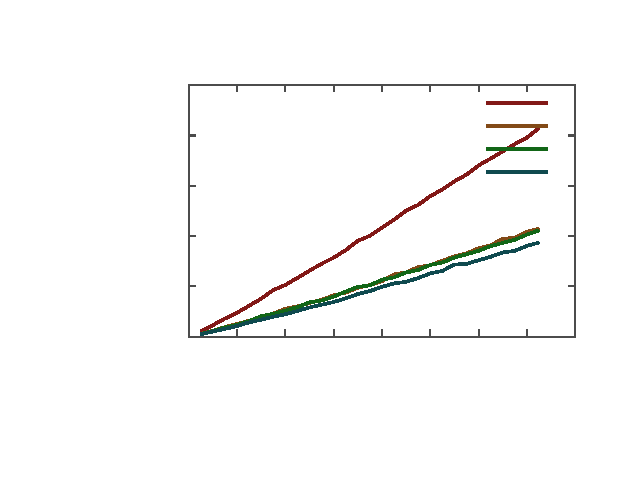
\includegraphics{./graficos/quicksort-linux-opt}}%
    \gplfronttext
  \end{picture}%
\endgroup

	\end{center}
\end{frame}

\begin{frame}
\vspace{2em}
\textbf{Representante de $\boldsymbol{O(n^3)}$}
	\begin{center}
		% GNUPLOT: LaTeX picture with Postscript
\begingroup
  \makeatletter
  \providecommand\color[2][]{%
    \GenericError{(gnuplot) \space\space\space\@spaces}{%
      Package color not loaded in conjunction with
      terminal option `colourtext'%
    }{See the gnuplot documentation for explanation.%
    }{Either use 'blacktext' in gnuplot or load the package
      color.sty in LaTeX.}%
    \renewcommand\color[2][]{}%
  }%
  \providecommand\includegraphics[2][]{%
    \GenericError{(gnuplot) \space\space\space\@spaces}{%
      Package graphicx or graphics not loaded%
    }{See the gnuplot documentation for explanation.%
    }{The gnuplot epslatex terminal needs graphicx.sty or graphics.sty.}%
    \renewcommand\includegraphics[2][]{}%
  }%
  \providecommand\rotatebox[2]{#2}%
  \@ifundefined{ifGPcolor}{%
    \newif\ifGPcolor
    \GPcolortrue
  }{}%
  \@ifundefined{ifGPblacktext}{%
    \newif\ifGPblacktext
    \GPblacktextfalse
  }{}%
  % define a \g@addto@macro without @ in the name:
  \let\gplgaddtomacro\g@addto@macro
  % define empty templates for all commands taking text:
  \gdef\gplbacktext{}%
  \gdef\gplfronttext{}%
  \makeatother
  \ifGPblacktext
    % no textcolor at all
    \def\colorrgb#1{}%
    \def\colorgray#1{}%
  \else
    % gray or color?
    \ifGPcolor
      \def\colorrgb#1{\color[rgb]{#1}}%
      \def\colorgray#1{\color[gray]{#1}}%
      \expandafter\def\csname LTw\endcsname{\color{white}}%
      \expandafter\def\csname LTb\endcsname{\color{black}}%
      \expandafter\def\csname LTa\endcsname{\color{black}}%
      \expandafter\def\csname LT0\endcsname{\color[rgb]{1,0,0}}%
      \expandafter\def\csname LT1\endcsname{\color[rgb]{0,1,0}}%
      \expandafter\def\csname LT2\endcsname{\color[rgb]{0,0,1}}%
      \expandafter\def\csname LT3\endcsname{\color[rgb]{1,0,1}}%
      \expandafter\def\csname LT4\endcsname{\color[rgb]{0,1,1}}%
      \expandafter\def\csname LT5\endcsname{\color[rgb]{1,1,0}}%
      \expandafter\def\csname LT6\endcsname{\color[rgb]{0,0,0}}%
      \expandafter\def\csname LT7\endcsname{\color[rgb]{1,0.3,0}}%
      \expandafter\def\csname LT8\endcsname{\color[rgb]{0.5,0.5,0.5}}%
    \else
      % gray
      \def\colorrgb#1{\color{black}}%
      \def\colorgray#1{\color[gray]{#1}}%
      \expandafter\def\csname LTw\endcsname{\color{white}}%
      \expandafter\def\csname LTb\endcsname{\color{black}}%
      \expandafter\def\csname LTa\endcsname{\color{black}}%
      \expandafter\def\csname LT0\endcsname{\color{black}}%
      \expandafter\def\csname LT1\endcsname{\color{black}}%
      \expandafter\def\csname LT2\endcsname{\color{black}}%
      \expandafter\def\csname LT3\endcsname{\color{black}}%
      \expandafter\def\csname LT4\endcsname{\color{black}}%
      \expandafter\def\csname LT5\endcsname{\color{black}}%
      \expandafter\def\csname LT6\endcsname{\color{black}}%
      \expandafter\def\csname LT7\endcsname{\color{black}}%
      \expandafter\def\csname LT8\endcsname{\color{black}}%
    \fi
  \fi
    \setlength{\unitlength}{0.0500bp}%
    \ifx\gptboxheight\undefined%
      \newlength{\gptboxheight}%
      \newlength{\gptboxwidth}%
      \newsavebox{\gptboxtext}%
    \fi%
    \setlength{\fboxrule}{0.5pt}%
    \setlength{\fboxsep}{1pt}%
\begin{picture}(5760.00,4320.00)%
    \gplgaddtomacro\gplbacktext{%
      \colorrgb{0.30,0.30,0.30}%
      \put(1122,1060){\makebox(0,0)[r]{\strut{}$\textcolor{text}{0}$}}%
      \colorrgb{0.30,0.30,0.30}%
      \put(1122,1320){\makebox(0,0)[r]{\strut{}$\textcolor{text}{2}$}}%
      \colorrgb{0.30,0.30,0.30}%
      \put(1122,1580){\makebox(0,0)[r]{\strut{}$\textcolor{text}{4}$}}%
      \colorrgb{0.30,0.30,0.30}%
      \put(1122,1840){\makebox(0,0)[r]{\strut{}$\textcolor{text}{6}$}}%
      \colorrgb{0.30,0.30,0.30}%
      \put(1122,2100){\makebox(0,0)[r]{\strut{}$\textcolor{text}{8}$}}%
      \colorrgb{0.30,0.30,0.30}%
      \put(1122,2360){\makebox(0,0)[r]{\strut{}$\textcolor{text}{10}$}}%
      \colorrgb{0.30,0.30,0.30}%
      \put(1122,2619){\makebox(0,0)[r]{\strut{}$\textcolor{text}{12}$}}%
      \colorrgb{0.30,0.30,0.30}%
      \put(1122,2879){\makebox(0,0)[r]{\strut{}$\textcolor{text}{14}$}}%
      \colorrgb{0.30,0.30,0.30}%
      \put(1122,3139){\makebox(0,0)[r]{\strut{}$\textcolor{text}{16}$}}%
      \colorrgb{0.30,0.30,0.30}%
      \put(1122,3399){\makebox(0,0)[r]{\strut{}$\textcolor{text}{18}$}}%
      \colorrgb{0.30,0.30,0.30}%
      \put(1122,3659){\makebox(0,0)[r]{\strut{}$\textcolor{text}{20}$}}%
      \colorrgb{0.30,0.30,0.30}%
      \put(1254,928){\rotatebox{45}{\makebox(0,0)[r]{\strut{}$\textcolor{text}{0}$}}}%
      \colorrgb{0.30,0.30,0.30}%
      \put(1768,928){\rotatebox{45}{\makebox(0,0)[r]{\strut{}$\textcolor{text}{200}$}}}%
      \colorrgb{0.30,0.30,0.30}%
      \put(2281,928){\rotatebox{45}{\makebox(0,0)[r]{\strut{}$\textcolor{text}{400}$}}}%
      \colorrgb{0.30,0.30,0.30}%
      \put(2795,928){\rotatebox{45}{\makebox(0,0)[r]{\strut{}$\textcolor{text}{600}$}}}%
      \colorrgb{0.30,0.30,0.30}%
      \put(3309,928){\rotatebox{45}{\makebox(0,0)[r]{\strut{}$\textcolor{text}{800}$}}}%
      \colorrgb{0.30,0.30,0.30}%
      \put(3822,928){\rotatebox{45}{\makebox(0,0)[r]{\strut{}$\textcolor{text}{1000}$}}}%
      \colorrgb{0.30,0.30,0.30}%
      \put(4336,928){\rotatebox{45}{\makebox(0,0)[r]{\strut{}$\textcolor{text}{1200}$}}}%
      \colorrgb{0.30,0.30,0.30}%
      \put(4849,928){\rotatebox{45}{\makebox(0,0)[r]{\strut{}$\textcolor{text}{1400}$}}}%
      \colorrgb{0.30,0.30,0.30}%
      \put(5363,928){\rotatebox{45}{\makebox(0,0)[r]{\strut{}$\textcolor{text}{1600}$}}}%
    }%
    \gplgaddtomacro\gplfronttext{%
      \colorrgb{0.30,0.30,0.30}%
      \put(220,2359){\rotatebox{-270}{\makebox(0,0){\strut{}Tiempo de ejecución (s)}}}%
      \colorrgb{0.30,0.30,0.30}%
      \put(3308,220){\makebox(0,0){\strut{}Tamaño del vector (elementos)}}%
      \colorrgb{0.30,0.30,0.30}%
      \put(3308,3989){\makebox(0,0){\strut{}Comparación floyd en macOS y Linux}}%
      \csname LTb\endcsname%
      \put(4376,3486){\makebox(0,0)[r]{\strut{}Linux}}%
      \csname LTb\endcsname%
      \put(4376,3266){\makebox(0,0)[r]{\strut{}Mac}}%
    }%
    \gplbacktext
    \put(0,0){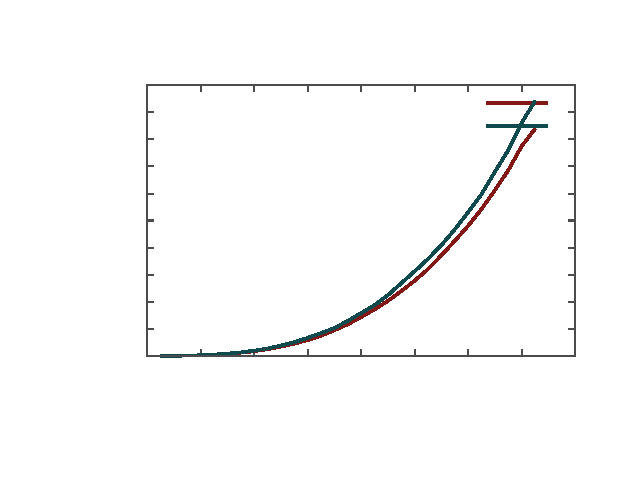
\includegraphics{./graficos/floyd-maclinux}}%
    \gplfronttext
  \end{picture}%
\endgroup

	\end{center}
\end{frame}

\begin{frame}
\vspace{2em}
\textbf{Representante de $\boldsymbol{O(n^3)}$}
	\begin{center}
		% GNUPLOT: LaTeX picture with Postscript
\begingroup
  \makeatletter
  \providecommand\color[2][]{%
    \GenericError{(gnuplot) \space\space\space\@spaces}{%
      Package color not loaded in conjunction with
      terminal option `colourtext'%
    }{See the gnuplot documentation for explanation.%
    }{Either use 'blacktext' in gnuplot or load the package
      color.sty in LaTeX.}%
    \renewcommand\color[2][]{}%
  }%
  \providecommand\includegraphics[2][]{%
    \GenericError{(gnuplot) \space\space\space\@spaces}{%
      Package graphicx or graphics not loaded%
    }{See the gnuplot documentation for explanation.%
    }{The gnuplot epslatex terminal needs graphicx.sty or graphics.sty.}%
    \renewcommand\includegraphics[2][]{}%
  }%
  \providecommand\rotatebox[2]{#2}%
  \@ifundefined{ifGPcolor}{%
    \newif\ifGPcolor
    \GPcolortrue
  }{}%
  \@ifundefined{ifGPblacktext}{%
    \newif\ifGPblacktext
    \GPblacktextfalse
  }{}%
  % define a \g@addto@macro without @ in the name:
  \let\gplgaddtomacro\g@addto@macro
  % define empty templates for all commands taking text:
  \gdef\gplbacktext{}%
  \gdef\gplfronttext{}%
  \makeatother
  \ifGPblacktext
    % no textcolor at all
    \def\colorrgb#1{}%
    \def\colorgray#1{}%
  \else
    % gray or color?
    \ifGPcolor
      \def\colorrgb#1{\color[rgb]{#1}}%
      \def\colorgray#1{\color[gray]{#1}}%
      \expandafter\def\csname LTw\endcsname{\color{white}}%
      \expandafter\def\csname LTb\endcsname{\color{black}}%
      \expandafter\def\csname LTa\endcsname{\color{black}}%
      \expandafter\def\csname LT0\endcsname{\color[rgb]{1,0,0}}%
      \expandafter\def\csname LT1\endcsname{\color[rgb]{0,1,0}}%
      \expandafter\def\csname LT2\endcsname{\color[rgb]{0,0,1}}%
      \expandafter\def\csname LT3\endcsname{\color[rgb]{1,0,1}}%
      \expandafter\def\csname LT4\endcsname{\color[rgb]{0,1,1}}%
      \expandafter\def\csname LT5\endcsname{\color[rgb]{1,1,0}}%
      \expandafter\def\csname LT6\endcsname{\color[rgb]{0,0,0}}%
      \expandafter\def\csname LT7\endcsname{\color[rgb]{1,0.3,0}}%
      \expandafter\def\csname LT8\endcsname{\color[rgb]{0.5,0.5,0.5}}%
    \else
      % gray
      \def\colorrgb#1{\color{black}}%
      \def\colorgray#1{\color[gray]{#1}}%
      \expandafter\def\csname LTw\endcsname{\color{white}}%
      \expandafter\def\csname LTb\endcsname{\color{black}}%
      \expandafter\def\csname LTa\endcsname{\color{black}}%
      \expandafter\def\csname LT0\endcsname{\color{black}}%
      \expandafter\def\csname LT1\endcsname{\color{black}}%
      \expandafter\def\csname LT2\endcsname{\color{black}}%
      \expandafter\def\csname LT3\endcsname{\color{black}}%
      \expandafter\def\csname LT4\endcsname{\color{black}}%
      \expandafter\def\csname LT5\endcsname{\color{black}}%
      \expandafter\def\csname LT6\endcsname{\color{black}}%
      \expandafter\def\csname LT7\endcsname{\color{black}}%
      \expandafter\def\csname LT8\endcsname{\color{black}}%
    \fi
  \fi
    \setlength{\unitlength}{0.0500bp}%
    \ifx\gptboxheight\undefined%
      \newlength{\gptboxheight}%
      \newlength{\gptboxwidth}%
      \newsavebox{\gptboxtext}%
    \fi%
    \setlength{\fboxrule}{0.5pt}%
    \setlength{\fboxsep}{1pt}%
\begin{picture}(5760.00,4320.00)%
    \gplgaddtomacro\gplbacktext{%
      \colorrgb{0.30,0.30,0.30}%
      \put(1122,1060){\makebox(0,0)[r]{\strut{}$\textcolor{text}{0}$}}%
      \colorrgb{0.30,0.30,0.30}%
      \put(1122,1349){\makebox(0,0)[r]{\strut{}$\textcolor{text}{2}$}}%
      \colorrgb{0.30,0.30,0.30}%
      \put(1122,1638){\makebox(0,0)[r]{\strut{}$\textcolor{text}{4}$}}%
      \colorrgb{0.30,0.30,0.30}%
      \put(1122,1926){\makebox(0,0)[r]{\strut{}$\textcolor{text}{6}$}}%
      \colorrgb{0.30,0.30,0.30}%
      \put(1122,2215){\makebox(0,0)[r]{\strut{}$\textcolor{text}{8}$}}%
      \colorrgb{0.30,0.30,0.30}%
      \put(1122,2504){\makebox(0,0)[r]{\strut{}$\textcolor{text}{10}$}}%
      \colorrgb{0.30,0.30,0.30}%
      \put(1122,2793){\makebox(0,0)[r]{\strut{}$\textcolor{text}{12}$}}%
      \colorrgb{0.30,0.30,0.30}%
      \put(1122,3081){\makebox(0,0)[r]{\strut{}$\textcolor{text}{14}$}}%
      \colorrgb{0.30,0.30,0.30}%
      \put(1122,3370){\makebox(0,0)[r]{\strut{}$\textcolor{text}{16}$}}%
      \colorrgb{0.30,0.30,0.30}%
      \put(1122,3659){\makebox(0,0)[r]{\strut{}$\textcolor{text}{18}$}}%
      \colorrgb{0.30,0.30,0.30}%
      \put(1254,928){\rotatebox{45}{\makebox(0,0)[r]{\strut{}$\textcolor{text}{0}$}}}%
      \colorrgb{0.30,0.30,0.30}%
      \put(1768,928){\rotatebox{45}{\makebox(0,0)[r]{\strut{}$\textcolor{text}{200}$}}}%
      \colorrgb{0.30,0.30,0.30}%
      \put(2281,928){\rotatebox{45}{\makebox(0,0)[r]{\strut{}$\textcolor{text}{400}$}}}%
      \colorrgb{0.30,0.30,0.30}%
      \put(2795,928){\rotatebox{45}{\makebox(0,0)[r]{\strut{}$\textcolor{text}{600}$}}}%
      \colorrgb{0.30,0.30,0.30}%
      \put(3309,928){\rotatebox{45}{\makebox(0,0)[r]{\strut{}$\textcolor{text}{800}$}}}%
      \colorrgb{0.30,0.30,0.30}%
      \put(3822,928){\rotatebox{45}{\makebox(0,0)[r]{\strut{}$\textcolor{text}{1000}$}}}%
      \colorrgb{0.30,0.30,0.30}%
      \put(4336,928){\rotatebox{45}{\makebox(0,0)[r]{\strut{}$\textcolor{text}{1200}$}}}%
      \colorrgb{0.30,0.30,0.30}%
      \put(4849,928){\rotatebox{45}{\makebox(0,0)[r]{\strut{}$\textcolor{text}{1400}$}}}%
      \colorrgb{0.30,0.30,0.30}%
      \put(5363,928){\rotatebox{45}{\makebox(0,0)[r]{\strut{}$\textcolor{text}{1600}$}}}%
    }%
    \gplgaddtomacro\gplfronttext{%
      \colorrgb{0.30,0.30,0.30}%
      \put(220,2359){\rotatebox{-270}{\makebox(0,0){\strut{}Tiempo de ejecución (s)}}}%
      \colorrgb{0.30,0.30,0.30}%
      \put(3308,220){\makebox(0,0){\strut{}Tamaño del vector (elementos)}}%
      \colorrgb{0.30,0.30,0.30}%
      \put(3308,3989){\makebox(0,0){\strut{}Comparación floyd en Linux con distinta optimización}}%
      \csname LTb\endcsname%
      \put(4376,3486){\makebox(0,0)[r]{\strut{}O0}}%
      \csname LTb\endcsname%
      \put(4376,3266){\makebox(0,0)[r]{\strut{}O1}}%
      \csname LTb\endcsname%
      \put(4376,3046){\makebox(0,0)[r]{\strut{}O2}}%
      \csname LTb\endcsname%
      \put(4376,2826){\makebox(0,0)[r]{\strut{}O3}}%
    }%
    \gplbacktext
    \put(0,0){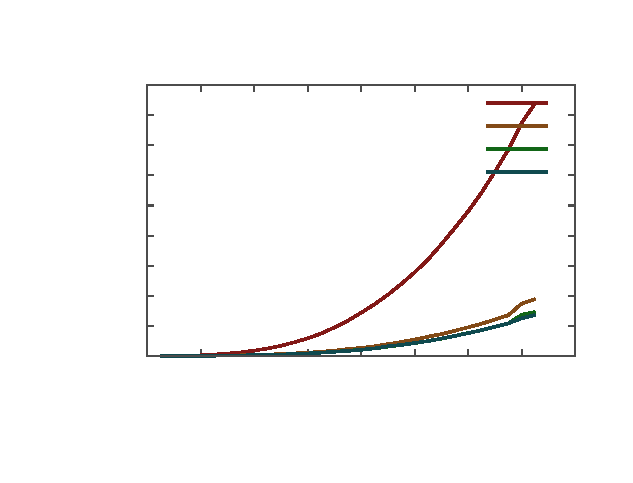
\includegraphics{./graficos/floyd-linux-opt}}%
    \gplfronttext
  \end{picture}%
\endgroup

	\end{center}
\end{frame}

\begin{frame}
\vspace{2em}
\textbf{Representante de $\boldsymbol{O(2^n)}$}
	\begin{center}
		% GNUPLOT: LaTeX picture with Postscript
\begingroup
  \makeatletter
  \providecommand\color[2][]{%
    \GenericError{(gnuplot) \space\space\space\@spaces}{%
      Package color not loaded in conjunction with
      terminal option `colourtext'%
    }{See the gnuplot documentation for explanation.%
    }{Either use 'blacktext' in gnuplot or load the package
      color.sty in LaTeX.}%
    \renewcommand\color[2][]{}%
  }%
  \providecommand\includegraphics[2][]{%
    \GenericError{(gnuplot) \space\space\space\@spaces}{%
      Package graphicx or graphics not loaded%
    }{See the gnuplot documentation for explanation.%
    }{The gnuplot epslatex terminal needs graphicx.sty or graphics.sty.}%
    \renewcommand\includegraphics[2][]{}%
  }%
  \providecommand\rotatebox[2]{#2}%
  \@ifundefined{ifGPcolor}{%
    \newif\ifGPcolor
    \GPcolortrue
  }{}%
  \@ifundefined{ifGPblacktext}{%
    \newif\ifGPblacktext
    \GPblacktextfalse
  }{}%
  % define a \g@addto@macro without @ in the name:
  \let\gplgaddtomacro\g@addto@macro
  % define empty templates for all commands taking text:
  \gdef\gplbacktext{}%
  \gdef\gplfronttext{}%
  \makeatother
  \ifGPblacktext
    % no textcolor at all
    \def\colorrgb#1{}%
    \def\colorgray#1{}%
  \else
    % gray or color?
    \ifGPcolor
      \def\colorrgb#1{\color[rgb]{#1}}%
      \def\colorgray#1{\color[gray]{#1}}%
      \expandafter\def\csname LTw\endcsname{\color{white}}%
      \expandafter\def\csname LTb\endcsname{\color{black}}%
      \expandafter\def\csname LTa\endcsname{\color{black}}%
      \expandafter\def\csname LT0\endcsname{\color[rgb]{1,0,0}}%
      \expandafter\def\csname LT1\endcsname{\color[rgb]{0,1,0}}%
      \expandafter\def\csname LT2\endcsname{\color[rgb]{0,0,1}}%
      \expandafter\def\csname LT3\endcsname{\color[rgb]{1,0,1}}%
      \expandafter\def\csname LT4\endcsname{\color[rgb]{0,1,1}}%
      \expandafter\def\csname LT5\endcsname{\color[rgb]{1,1,0}}%
      \expandafter\def\csname LT6\endcsname{\color[rgb]{0,0,0}}%
      \expandafter\def\csname LT7\endcsname{\color[rgb]{1,0.3,0}}%
      \expandafter\def\csname LT8\endcsname{\color[rgb]{0.5,0.5,0.5}}%
    \else
      % gray
      \def\colorrgb#1{\color{black}}%
      \def\colorgray#1{\color[gray]{#1}}%
      \expandafter\def\csname LTw\endcsname{\color{white}}%
      \expandafter\def\csname LTb\endcsname{\color{black}}%
      \expandafter\def\csname LTa\endcsname{\color{black}}%
      \expandafter\def\csname LT0\endcsname{\color{black}}%
      \expandafter\def\csname LT1\endcsname{\color{black}}%
      \expandafter\def\csname LT2\endcsname{\color{black}}%
      \expandafter\def\csname LT3\endcsname{\color{black}}%
      \expandafter\def\csname LT4\endcsname{\color{black}}%
      \expandafter\def\csname LT5\endcsname{\color{black}}%
      \expandafter\def\csname LT6\endcsname{\color{black}}%
      \expandafter\def\csname LT7\endcsname{\color{black}}%
      \expandafter\def\csname LT8\endcsname{\color{black}}%
    \fi
  \fi
    \setlength{\unitlength}{0.0500bp}%
    \ifx\gptboxheight\undefined%
      \newlength{\gptboxheight}%
      \newlength{\gptboxwidth}%
      \newsavebox{\gptboxtext}%
    \fi%
    \setlength{\fboxrule}{0.5pt}%
    \setlength{\fboxsep}{1pt}%
\begin{picture}(5760.00,4320.00)%
    \gplgaddtomacro\gplbacktext{%
      \colorrgb{0.30,0.30,0.30}%
      \put(990,873){\makebox(0,0)[r]{\strut{}$\textcolor{text}{0}$}}%
      \colorrgb{0.30,0.30,0.30}%
      \put(990,1271){\makebox(0,0)[r]{\strut{}$\textcolor{text}{1}$}}%
      \colorrgb{0.30,0.30,0.30}%
      \put(990,1669){\makebox(0,0)[r]{\strut{}$\textcolor{text}{2}$}}%
      \colorrgb{0.30,0.30,0.30}%
      \put(990,2067){\makebox(0,0)[r]{\strut{}$\textcolor{text}{3}$}}%
      \colorrgb{0.30,0.30,0.30}%
      \put(990,2465){\makebox(0,0)[r]{\strut{}$\textcolor{text}{4}$}}%
      \colorrgb{0.30,0.30,0.30}%
      \put(990,2863){\makebox(0,0)[r]{\strut{}$\textcolor{text}{5}$}}%
      \colorrgb{0.30,0.30,0.30}%
      \put(990,3261){\makebox(0,0)[r]{\strut{}$\textcolor{text}{6}$}}%
      \colorrgb{0.30,0.30,0.30}%
      \put(990,3659){\makebox(0,0)[r]{\strut{}$\textcolor{text}{7}$}}%
      \colorrgb{0.30,0.30,0.30}%
      \put(1122,741){\rotatebox{45}{\makebox(0,0)[r]{\strut{}$\textcolor{text}{5}$}}}%
      \colorrgb{0.30,0.30,0.30}%
      \put(1970,741){\rotatebox{45}{\makebox(0,0)[r]{\strut{}$\textcolor{text}{10}$}}}%
      \colorrgb{0.30,0.30,0.30}%
      \put(2818,741){\rotatebox{45}{\makebox(0,0)[r]{\strut{}$\textcolor{text}{15}$}}}%
      \colorrgb{0.30,0.30,0.30}%
      \put(3667,741){\rotatebox{45}{\makebox(0,0)[r]{\strut{}$\textcolor{text}{20}$}}}%
      \colorrgb{0.30,0.30,0.30}%
      \put(4515,741){\rotatebox{45}{\makebox(0,0)[r]{\strut{}$\textcolor{text}{25}$}}}%
      \colorrgb{0.30,0.30,0.30}%
      \put(5363,741){\rotatebox{45}{\makebox(0,0)[r]{\strut{}$\textcolor{text}{30}$}}}%
    }%
    \gplgaddtomacro\gplfronttext{%
      \colorrgb{0.30,0.30,0.30}%
      \put(220,2266){\rotatebox{-270}{\makebox(0,0){\strut{}Tiempo de ejecución (s)}}}%
      \colorrgb{0.30,0.30,0.30}%
      \put(3242,220){\makebox(0,0){\strut{}Tamaño del vector (elementos)}}%
      \colorrgb{0.30,0.30,0.30}%
      \put(3242,3989){\makebox(0,0){\strut{}Comparación hanoi en macOS y Linux}}%
      \csname LTb\endcsname%
      \put(4376,3486){\makebox(0,0)[r]{\strut{}Linux}}%
      \csname LTb\endcsname%
      \put(4376,3266){\makebox(0,0)[r]{\strut{}Mac}}%
    }%
    \gplbacktext
    \put(0,0){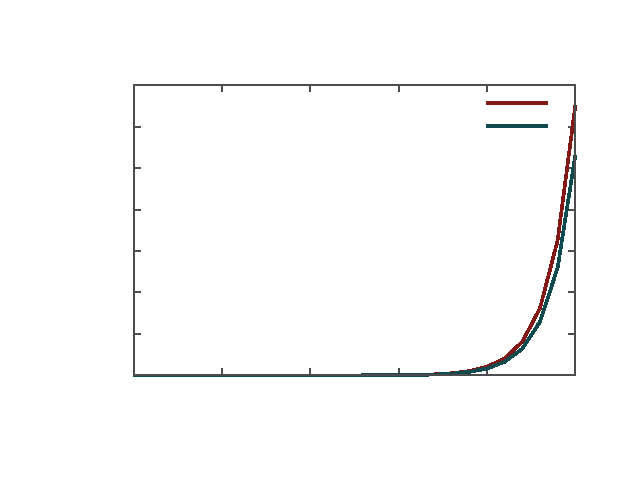
\includegraphics{./graficos/hanoi-maclinux}}%
    \gplfronttext
  \end{picture}%
\endgroup

	\end{center}
\end{frame}

\begin{frame}
\vspace{2em}
\textbf{Representante de $\boldsymbol{O(2^n)}$}
	\begin{center}
		% GNUPLOT: LaTeX picture with Postscript
\begingroup
  \makeatletter
  \providecommand\color[2][]{%
    \GenericError{(gnuplot) \space\space\space\@spaces}{%
      Package color not loaded in conjunction with
      terminal option `colourtext'%
    }{See the gnuplot documentation for explanation.%
    }{Either use 'blacktext' in gnuplot or load the package
      color.sty in LaTeX.}%
    \renewcommand\color[2][]{}%
  }%
  \providecommand\includegraphics[2][]{%
    \GenericError{(gnuplot) \space\space\space\@spaces}{%
      Package graphicx or graphics not loaded%
    }{See the gnuplot documentation for explanation.%
    }{The gnuplot epslatex terminal needs graphicx.sty or graphics.sty.}%
    \renewcommand\includegraphics[2][]{}%
  }%
  \providecommand\rotatebox[2]{#2}%
  \@ifundefined{ifGPcolor}{%
    \newif\ifGPcolor
    \GPcolortrue
  }{}%
  \@ifundefined{ifGPblacktext}{%
    \newif\ifGPblacktext
    \GPblacktextfalse
  }{}%
  % define a \g@addto@macro without @ in the name:
  \let\gplgaddtomacro\g@addto@macro
  % define empty templates for all commands taking text:
  \gdef\gplbacktext{}%
  \gdef\gplfronttext{}%
  \makeatother
  \ifGPblacktext
    % no textcolor at all
    \def\colorrgb#1{}%
    \def\colorgray#1{}%
  \else
    % gray or color?
    \ifGPcolor
      \def\colorrgb#1{\color[rgb]{#1}}%
      \def\colorgray#1{\color[gray]{#1}}%
      \expandafter\def\csname LTw\endcsname{\color{white}}%
      \expandafter\def\csname LTb\endcsname{\color{black}}%
      \expandafter\def\csname LTa\endcsname{\color{black}}%
      \expandafter\def\csname LT0\endcsname{\color[rgb]{1,0,0}}%
      \expandafter\def\csname LT1\endcsname{\color[rgb]{0,1,0}}%
      \expandafter\def\csname LT2\endcsname{\color[rgb]{0,0,1}}%
      \expandafter\def\csname LT3\endcsname{\color[rgb]{1,0,1}}%
      \expandafter\def\csname LT4\endcsname{\color[rgb]{0,1,1}}%
      \expandafter\def\csname LT5\endcsname{\color[rgb]{1,1,0}}%
      \expandafter\def\csname LT6\endcsname{\color[rgb]{0,0,0}}%
      \expandafter\def\csname LT7\endcsname{\color[rgb]{1,0.3,0}}%
      \expandafter\def\csname LT8\endcsname{\color[rgb]{0.5,0.5,0.5}}%
    \else
      % gray
      \def\colorrgb#1{\color{black}}%
      \def\colorgray#1{\color[gray]{#1}}%
      \expandafter\def\csname LTw\endcsname{\color{white}}%
      \expandafter\def\csname LTb\endcsname{\color{black}}%
      \expandafter\def\csname LTa\endcsname{\color{black}}%
      \expandafter\def\csname LT0\endcsname{\color{black}}%
      \expandafter\def\csname LT1\endcsname{\color{black}}%
      \expandafter\def\csname LT2\endcsname{\color{black}}%
      \expandafter\def\csname LT3\endcsname{\color{black}}%
      \expandafter\def\csname LT4\endcsname{\color{black}}%
      \expandafter\def\csname LT5\endcsname{\color{black}}%
      \expandafter\def\csname LT6\endcsname{\color{black}}%
      \expandafter\def\csname LT7\endcsname{\color{black}}%
      \expandafter\def\csname LT8\endcsname{\color{black}}%
    \fi
  \fi
    \setlength{\unitlength}{0.0500bp}%
    \ifx\gptboxheight\undefined%
      \newlength{\gptboxheight}%
      \newlength{\gptboxwidth}%
      \newsavebox{\gptboxtext}%
    \fi%
    \setlength{\fboxrule}{0.5pt}%
    \setlength{\fboxsep}{1pt}%
\begin{picture}(5760.00,4320.00)%
    \gplgaddtomacro\gplbacktext{%
      \colorrgb{0.30,0.30,0.30}%
      \put(990,873){\makebox(0,0)[r]{\strut{}$\textcolor{text}{0}$}}%
      \colorrgb{0.30,0.30,0.30}%
      \put(990,1271){\makebox(0,0)[r]{\strut{}$\textcolor{text}{1}$}}%
      \colorrgb{0.30,0.30,0.30}%
      \put(990,1669){\makebox(0,0)[r]{\strut{}$\textcolor{text}{2}$}}%
      \colorrgb{0.30,0.30,0.30}%
      \put(990,2067){\makebox(0,0)[r]{\strut{}$\textcolor{text}{3}$}}%
      \colorrgb{0.30,0.30,0.30}%
      \put(990,2465){\makebox(0,0)[r]{\strut{}$\textcolor{text}{4}$}}%
      \colorrgb{0.30,0.30,0.30}%
      \put(990,2863){\makebox(0,0)[r]{\strut{}$\textcolor{text}{5}$}}%
      \colorrgb{0.30,0.30,0.30}%
      \put(990,3261){\makebox(0,0)[r]{\strut{}$\textcolor{text}{6}$}}%
      \colorrgb{0.30,0.30,0.30}%
      \put(990,3659){\makebox(0,0)[r]{\strut{}$\textcolor{text}{7}$}}%
      \colorrgb{0.30,0.30,0.30}%
      \put(1122,741){\rotatebox{45}{\makebox(0,0)[r]{\strut{}$\textcolor{text}{5}$}}}%
      \colorrgb{0.30,0.30,0.30}%
      \put(1970,741){\rotatebox{45}{\makebox(0,0)[r]{\strut{}$\textcolor{text}{10}$}}}%
      \colorrgb{0.30,0.30,0.30}%
      \put(2818,741){\rotatebox{45}{\makebox(0,0)[r]{\strut{}$\textcolor{text}{15}$}}}%
      \colorrgb{0.30,0.30,0.30}%
      \put(3667,741){\rotatebox{45}{\makebox(0,0)[r]{\strut{}$\textcolor{text}{20}$}}}%
      \colorrgb{0.30,0.30,0.30}%
      \put(4515,741){\rotatebox{45}{\makebox(0,0)[r]{\strut{}$\textcolor{text}{25}$}}}%
      \colorrgb{0.30,0.30,0.30}%
      \put(5363,741){\rotatebox{45}{\makebox(0,0)[r]{\strut{}$\textcolor{text}{30}$}}}%
    }%
    \gplgaddtomacro\gplfronttext{%
      \colorrgb{0.30,0.30,0.30}%
      \put(220,2266){\rotatebox{-270}{\makebox(0,0){\strut{}Tiempo de ejecución (s)}}}%
      \colorrgb{0.30,0.30,0.30}%
      \put(3242,220){\makebox(0,0){\strut{}Tamaño del vector (elementos)}}%
      \colorrgb{0.30,0.30,0.30}%
      \put(3242,3989){\makebox(0,0){\strut{}Comparación hanoi en Linux con distinta optimización}}%
      \csname LTb\endcsname%
      \put(4376,3486){\makebox(0,0)[r]{\strut{}O0}}%
      \csname LTb\endcsname%
      \put(4376,3266){\makebox(0,0)[r]{\strut{}O1}}%
      \csname LTb\endcsname%
      \put(4376,3046){\makebox(0,0)[r]{\strut{}O2}}%
      \csname LTb\endcsname%
      \put(4376,2826){\makebox(0,0)[r]{\strut{}O3}}%
    }%
    \gplbacktext
    \put(0,0){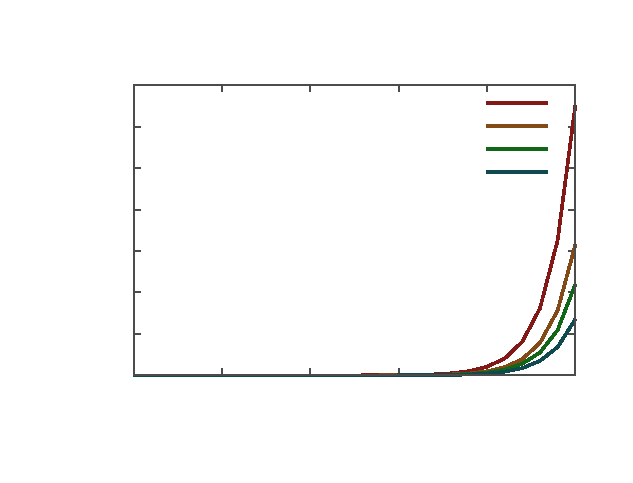
\includegraphics{./graficos/hanoi-linux-opt}}%
    \gplfronttext
  \end{picture}%
\endgroup

	\end{center}
\end{frame}

\begin{frame}{Eficiencia híbrida}
	A continuación se recogen los gráficos que muestran tanto la eficiencia empírica como la función ajustada o \textit{eficiencia híbrida} de cada algoritmo.	
	\vskip 0.5 cm
	También se muestran, para cada algoritmo, las constantes ocultas en la expresión de la eficiencia teórica.
\end{frame}

\begin{frame}
    \vspace{2.5em}
    \textbf{Burbuja}
	\fontsize{8pt}{7.2}\selectfont
	\begin{center}
		% GNUPLOT: LaTeX picture with Postscript
\begingroup
  \makeatletter
  \providecommand\color[2][]{%
    \GenericError{(gnuplot) \space\space\space\@spaces}{%
      Package color not loaded in conjunction with
      terminal option `colourtext'%
    }{See the gnuplot documentation for explanation.%
    }{Either use 'blacktext' in gnuplot or load the package
      color.sty in LaTeX.}%
    \renewcommand\color[2][]{}%
  }%
  \providecommand\includegraphics[2][]{%
    \GenericError{(gnuplot) \space\space\space\@spaces}{%
      Package graphicx or graphics not loaded%
    }{See the gnuplot documentation for explanation.%
    }{The gnuplot epslatex terminal needs graphicx.sty or graphics.sty.}%
    \renewcommand\includegraphics[2][]{}%
  }%
  \providecommand\rotatebox[2]{#2}%
  \@ifundefined{ifGPcolor}{%
    \newif\ifGPcolor
    \GPcolortrue
  }{}%
  \@ifundefined{ifGPblacktext}{%
    \newif\ifGPblacktext
    \GPblacktextfalse
  }{}%
  % define a \g@addto@macro without @ in the name:
  \let\gplgaddtomacro\g@addto@macro
  % define empty templates for all commands taking text:
  \gdef\gplbacktext{}%
  \gdef\gplfronttext{}%
  \makeatother
  \ifGPblacktext
    % no textcolor at all
    \def\colorrgb#1{}%
    \def\colorgray#1{}%
  \else
    % gray or color?
    \ifGPcolor
      \def\colorrgb#1{\color[rgb]{#1}}%
      \def\colorgray#1{\color[gray]{#1}}%
      \expandafter\def\csname LTw\endcsname{\color{white}}%
      \expandafter\def\csname LTb\endcsname{\color{black}}%
      \expandafter\def\csname LTa\endcsname{\color{black}}%
      \expandafter\def\csname LT0\endcsname{\color[rgb]{1,0,0}}%
      \expandafter\def\csname LT1\endcsname{\color[rgb]{0,1,0}}%
      \expandafter\def\csname LT2\endcsname{\color[rgb]{0,0,1}}%
      \expandafter\def\csname LT3\endcsname{\color[rgb]{1,0,1}}%
      \expandafter\def\csname LT4\endcsname{\color[rgb]{0,1,1}}%
      \expandafter\def\csname LT5\endcsname{\color[rgb]{1,1,0}}%
      \expandafter\def\csname LT6\endcsname{\color[rgb]{0,0,0}}%
      \expandafter\def\csname LT7\endcsname{\color[rgb]{1,0.3,0}}%
      \expandafter\def\csname LT8\endcsname{\color[rgb]{0.5,0.5,0.5}}%
    \else
      % gray
      \def\colorrgb#1{\color{black}}%
      \def\colorgray#1{\color[gray]{#1}}%
      \expandafter\def\csname LTw\endcsname{\color{white}}%
      \expandafter\def\csname LTb\endcsname{\color{black}}%
      \expandafter\def\csname LTa\endcsname{\color{black}}%
      \expandafter\def\csname LT0\endcsname{\color{black}}%
      \expandafter\def\csname LT1\endcsname{\color{black}}%
      \expandafter\def\csname LT2\endcsname{\color{black}}%
      \expandafter\def\csname LT3\endcsname{\color{black}}%
      \expandafter\def\csname LT4\endcsname{\color{black}}%
      \expandafter\def\csname LT5\endcsname{\color{black}}%
      \expandafter\def\csname LT6\endcsname{\color{black}}%
      \expandafter\def\csname LT7\endcsname{\color{black}}%
      \expandafter\def\csname LT8\endcsname{\color{black}}%
    \fi
  \fi
    \setlength{\unitlength}{0.0500bp}%
    \ifx\gptboxheight\undefined%
      \newlength{\gptboxheight}%
      \newlength{\gptboxwidth}%
      \newsavebox{\gptboxtext}%
    \fi%
    \setlength{\fboxrule}{0.5pt}%
    \setlength{\fboxsep}{1pt}%
\begin{picture}(5760.00,4320.00)%
    \gplgaddtomacro\gplbacktext{%
      \colorrgb{0.30,0.30,0.30}%
      \put(990,1153){\makebox(0,0)[r]{\strut{}$\textcolor{text}{0}$}}%
      \colorrgb{0.30,0.30,0.30}%
      \put(990,1466){\makebox(0,0)[r]{\strut{}$\textcolor{text}{1}$}}%
      \colorrgb{0.30,0.30,0.30}%
      \put(990,1780){\makebox(0,0)[r]{\strut{}$\textcolor{text}{2}$}}%
      \colorrgb{0.30,0.30,0.30}%
      \put(990,2093){\makebox(0,0)[r]{\strut{}$\textcolor{text}{3}$}}%
      \colorrgb{0.30,0.30,0.30}%
      \put(990,2406){\makebox(0,0)[r]{\strut{}$\textcolor{text}{4}$}}%
      \colorrgb{0.30,0.30,0.30}%
      \put(990,2719){\makebox(0,0)[r]{\strut{}$\textcolor{text}{5}$}}%
      \colorrgb{0.30,0.30,0.30}%
      \put(990,3033){\makebox(0,0)[r]{\strut{}$\textcolor{text}{6}$}}%
      \colorrgb{0.30,0.30,0.30}%
      \put(990,3346){\makebox(0,0)[r]{\strut{}$\textcolor{text}{7}$}}%
      \colorrgb{0.30,0.30,0.30}%
      \put(990,3659){\makebox(0,0)[r]{\strut{}$\textcolor{text}{8}$}}%
      \colorrgb{0.30,0.30,0.30}%
      \put(1122,1021){\rotatebox{45}{\makebox(0,0)[r]{\strut{}$\textcolor{text}{0}$}}}%
      \colorrgb{0.30,0.30,0.30}%
      \put(1546,1021){\rotatebox{45}{\makebox(0,0)[r]{\strut{}$\textcolor{text}{5000}$}}}%
      \colorrgb{0.30,0.30,0.30}%
      \put(1970,1021){\rotatebox{45}{\makebox(0,0)[r]{\strut{}$\textcolor{text}{10000}$}}}%
      \colorrgb{0.30,0.30,0.30}%
      \put(2394,1021){\rotatebox{45}{\makebox(0,0)[r]{\strut{}$\textcolor{text}{15000}$}}}%
      \colorrgb{0.30,0.30,0.30}%
      \put(2818,1021){\rotatebox{45}{\makebox(0,0)[r]{\strut{}$\textcolor{text}{20000}$}}}%
      \colorrgb{0.30,0.30,0.30}%
      \put(3243,1021){\rotatebox{45}{\makebox(0,0)[r]{\strut{}$\textcolor{text}{25000}$}}}%
      \colorrgb{0.30,0.30,0.30}%
      \put(3667,1021){\rotatebox{45}{\makebox(0,0)[r]{\strut{}$\textcolor{text}{30000}$}}}%
      \colorrgb{0.30,0.30,0.30}%
      \put(4091,1021){\rotatebox{45}{\makebox(0,0)[r]{\strut{}$\textcolor{text}{35000}$}}}%
      \colorrgb{0.30,0.30,0.30}%
      \put(4515,1021){\rotatebox{45}{\makebox(0,0)[r]{\strut{}$\textcolor{text}{40000}$}}}%
      \colorrgb{0.30,0.30,0.30}%
      \put(4939,1021){\rotatebox{45}{\makebox(0,0)[r]{\strut{}$\textcolor{text}{45000}$}}}%
      \colorrgb{0.30,0.30,0.30}%
      \put(5363,1021){\rotatebox{45}{\makebox(0,0)[r]{\strut{}$\textcolor{text}{50000}$}}}%
    }%
    \gplgaddtomacro\gplfronttext{%
      \colorrgb{0.30,0.30,0.30}%
      \put(220,2406){\rotatebox{-270}{\makebox(0,0){\strut{}Tiempo de ejecución (s)}}}%
      \colorrgb{0.30,0.30,0.30}%
      \put(3242,220){\makebox(0,0){\strut{}Tamaño del vector (elementos)}}%
      \colorrgb{0.30,0.30,0.30}%
      \put(3242,3989){\makebox(0,0){\strut{}Ajuste Burbuja}}%
      \csname LTb\endcsname%
      \put(4376,3486){\makebox(0,0)[r]{\strut{}3.19e-09$x^2$+-5.20e-06$x$+5.81e-04}}%
      \csname LTb\endcsname%
      \put(4376,3266){\makebox(0,0)[r]{\strut{}Burbuja}}%
    }%
    \gplbacktext
    \put(0,0){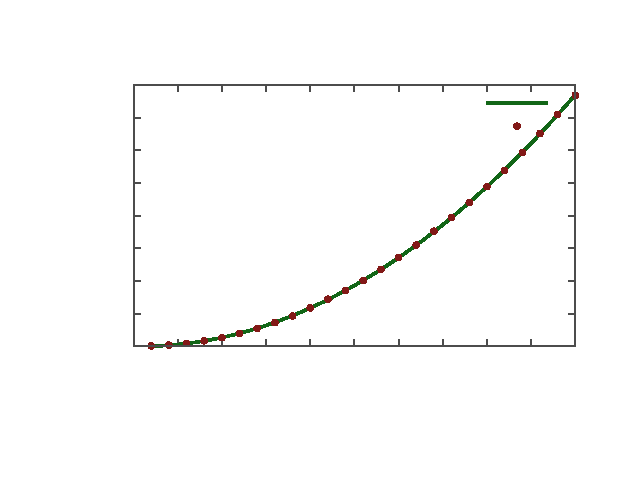
\includegraphics{./graficos/ajuste-burbuja}}%
    \gplfronttext
  \end{picture}%
\endgroup

	\end{center}
\end{frame}

\begin{frame}
    \vspace{2.5em}
    \textbf{Inserción}
	\fontsize{8pt}{7.2}\selectfont
	\begin{center}
		% GNUPLOT: LaTeX picture with Postscript
\begingroup
  \makeatletter
  \providecommand\color[2][]{%
    \GenericError{(gnuplot) \space\space\space\@spaces}{%
      Package color not loaded in conjunction with
      terminal option `colourtext'%
    }{See the gnuplot documentation for explanation.%
    }{Either use 'blacktext' in gnuplot or load the package
      color.sty in LaTeX.}%
    \renewcommand\color[2][]{}%
  }%
  \providecommand\includegraphics[2][]{%
    \GenericError{(gnuplot) \space\space\space\@spaces}{%
      Package graphicx or graphics not loaded%
    }{See the gnuplot documentation for explanation.%
    }{The gnuplot epslatex terminal needs graphicx.sty or graphics.sty.}%
    \renewcommand\includegraphics[2][]{}%
  }%
  \providecommand\rotatebox[2]{#2}%
  \@ifundefined{ifGPcolor}{%
    \newif\ifGPcolor
    \GPcolortrue
  }{}%
  \@ifundefined{ifGPblacktext}{%
    \newif\ifGPblacktext
    \GPblacktextfalse
  }{}%
  % define a \g@addto@macro without @ in the name:
  \let\gplgaddtomacro\g@addto@macro
  % define empty templates for all commands taking text:
  \gdef\gplbacktext{}%
  \gdef\gplfronttext{}%
  \makeatother
  \ifGPblacktext
    % no textcolor at all
    \def\colorrgb#1{}%
    \def\colorgray#1{}%
  \else
    % gray or color?
    \ifGPcolor
      \def\colorrgb#1{\color[rgb]{#1}}%
      \def\colorgray#1{\color[gray]{#1}}%
      \expandafter\def\csname LTw\endcsname{\color{white}}%
      \expandafter\def\csname LTb\endcsname{\color{black}}%
      \expandafter\def\csname LTa\endcsname{\color{black}}%
      \expandafter\def\csname LT0\endcsname{\color[rgb]{1,0,0}}%
      \expandafter\def\csname LT1\endcsname{\color[rgb]{0,1,0}}%
      \expandafter\def\csname LT2\endcsname{\color[rgb]{0,0,1}}%
      \expandafter\def\csname LT3\endcsname{\color[rgb]{1,0,1}}%
      \expandafter\def\csname LT4\endcsname{\color[rgb]{0,1,1}}%
      \expandafter\def\csname LT5\endcsname{\color[rgb]{1,1,0}}%
      \expandafter\def\csname LT6\endcsname{\color[rgb]{0,0,0}}%
      \expandafter\def\csname LT7\endcsname{\color[rgb]{1,0.3,0}}%
      \expandafter\def\csname LT8\endcsname{\color[rgb]{0.5,0.5,0.5}}%
    \else
      % gray
      \def\colorrgb#1{\color{black}}%
      \def\colorgray#1{\color[gray]{#1}}%
      \expandafter\def\csname LTw\endcsname{\color{white}}%
      \expandafter\def\csname LTb\endcsname{\color{black}}%
      \expandafter\def\csname LTa\endcsname{\color{black}}%
      \expandafter\def\csname LT0\endcsname{\color{black}}%
      \expandafter\def\csname LT1\endcsname{\color{black}}%
      \expandafter\def\csname LT2\endcsname{\color{black}}%
      \expandafter\def\csname LT3\endcsname{\color{black}}%
      \expandafter\def\csname LT4\endcsname{\color{black}}%
      \expandafter\def\csname LT5\endcsname{\color{black}}%
      \expandafter\def\csname LT6\endcsname{\color{black}}%
      \expandafter\def\csname LT7\endcsname{\color{black}}%
      \expandafter\def\csname LT8\endcsname{\color{black}}%
    \fi
  \fi
    \setlength{\unitlength}{0.0500bp}%
    \ifx\gptboxheight\undefined%
      \newlength{\gptboxheight}%
      \newlength{\gptboxwidth}%
      \newsavebox{\gptboxtext}%
    \fi%
    \setlength{\fboxrule}{0.5pt}%
    \setlength{\fboxsep}{1pt}%
\begin{picture}(5760.00,4320.00)%
    \gplgaddtomacro\gplbacktext{%
      \colorrgb{0.30,0.30,0.30}%
      \put(1254,1153){\makebox(0,0)[r]{\strut{}$\textcolor{text}{0}$}}%
      \colorrgb{0.30,0.30,0.30}%
      \put(1254,1571){\makebox(0,0)[r]{\strut{}$\textcolor{text}{0.5}$}}%
      \colorrgb{0.30,0.30,0.30}%
      \put(1254,1988){\makebox(0,0)[r]{\strut{}$\textcolor{text}{1}$}}%
      \colorrgb{0.30,0.30,0.30}%
      \put(1254,2406){\makebox(0,0)[r]{\strut{}$\textcolor{text}{1.5}$}}%
      \colorrgb{0.30,0.30,0.30}%
      \put(1254,2824){\makebox(0,0)[r]{\strut{}$\textcolor{text}{2}$}}%
      \colorrgb{0.30,0.30,0.30}%
      \put(1254,3241){\makebox(0,0)[r]{\strut{}$\textcolor{text}{2.5}$}}%
      \colorrgb{0.30,0.30,0.30}%
      \put(1254,3659){\makebox(0,0)[r]{\strut{}$\textcolor{text}{3}$}}%
      \colorrgb{0.30,0.30,0.30}%
      \put(1386,1021){\rotatebox{45}{\makebox(0,0)[r]{\strut{}$\textcolor{text}{0}$}}}%
      \colorrgb{0.30,0.30,0.30}%
      \put(1784,1021){\rotatebox{45}{\makebox(0,0)[r]{\strut{}$\textcolor{text}{5000}$}}}%
      \colorrgb{0.30,0.30,0.30}%
      \put(2181,1021){\rotatebox{45}{\makebox(0,0)[r]{\strut{}$\textcolor{text}{10000}$}}}%
      \colorrgb{0.30,0.30,0.30}%
      \put(2579,1021){\rotatebox{45}{\makebox(0,0)[r]{\strut{}$\textcolor{text}{15000}$}}}%
      \colorrgb{0.30,0.30,0.30}%
      \put(2977,1021){\rotatebox{45}{\makebox(0,0)[r]{\strut{}$\textcolor{text}{20000}$}}}%
      \colorrgb{0.30,0.30,0.30}%
      \put(3375,1021){\rotatebox{45}{\makebox(0,0)[r]{\strut{}$\textcolor{text}{25000}$}}}%
      \colorrgb{0.30,0.30,0.30}%
      \put(3772,1021){\rotatebox{45}{\makebox(0,0)[r]{\strut{}$\textcolor{text}{30000}$}}}%
      \colorrgb{0.30,0.30,0.30}%
      \put(4170,1021){\rotatebox{45}{\makebox(0,0)[r]{\strut{}$\textcolor{text}{35000}$}}}%
      \colorrgb{0.30,0.30,0.30}%
      \put(4568,1021){\rotatebox{45}{\makebox(0,0)[r]{\strut{}$\textcolor{text}{40000}$}}}%
      \colorrgb{0.30,0.30,0.30}%
      \put(4965,1021){\rotatebox{45}{\makebox(0,0)[r]{\strut{}$\textcolor{text}{45000}$}}}%
      \colorrgb{0.30,0.30,0.30}%
      \put(5363,1021){\rotatebox{45}{\makebox(0,0)[r]{\strut{}$\textcolor{text}{50000}$}}}%
    }%
    \gplgaddtomacro\gplfronttext{%
      \colorrgb{0.30,0.30,0.30}%
      \put(220,2406){\rotatebox{-270}{\makebox(0,0){\strut{}Tiempo de ejecución (s)}}}%
      \colorrgb{0.30,0.30,0.30}%
      \put(3374,220){\makebox(0,0){\strut{}Tamaño del vector (elementos)}}%
      \colorrgb{0.30,0.30,0.30}%
      \put(3374,3989){\makebox(0,0){\strut{}Ajuste Inserción}}%
      \csname LTb\endcsname%
      \put(4376,3486){\makebox(0,0)[r]{\strut{}1.14e-09$x^2$+-2.64e-06$x$+1.87e-02}}%
      \csname LTb\endcsname%
      \put(4376,3266){\makebox(0,0)[r]{\strut{}Inserción}}%
    }%
    \gplbacktext
    \put(0,0){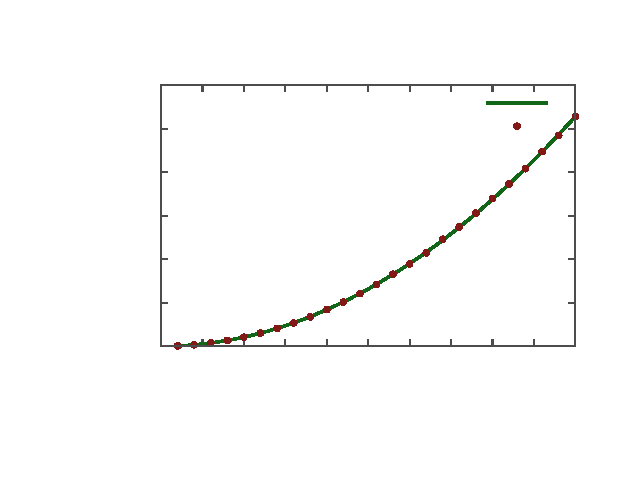
\includegraphics{./graficos/ajuste-insercion}}%
    \gplfronttext
  \end{picture}%
\endgroup

	\end{center}
\end{frame}

\begin{frame}
    \vspace{2.5em}
    \textbf{Selección}
	\fontsize{8pt}{7.2}\selectfont
	\begin{center}
		% GNUPLOT: LaTeX picture with Postscript
\begingroup
  \makeatletter
  \providecommand\color[2][]{%
    \GenericError{(gnuplot) \space\space\space\@spaces}{%
      Package color not loaded in conjunction with
      terminal option `colourtext'%
    }{See the gnuplot documentation for explanation.%
    }{Either use 'blacktext' in gnuplot or load the package
      color.sty in LaTeX.}%
    \renewcommand\color[2][]{}%
  }%
  \providecommand\includegraphics[2][]{%
    \GenericError{(gnuplot) \space\space\space\@spaces}{%
      Package graphicx or graphics not loaded%
    }{See the gnuplot documentation for explanation.%
    }{The gnuplot epslatex terminal needs graphicx.sty or graphics.sty.}%
    \renewcommand\includegraphics[2][]{}%
  }%
  \providecommand\rotatebox[2]{#2}%
  \@ifundefined{ifGPcolor}{%
    \newif\ifGPcolor
    \GPcolortrue
  }{}%
  \@ifundefined{ifGPblacktext}{%
    \newif\ifGPblacktext
    \GPblacktextfalse
  }{}%
  % define a \g@addto@macro without @ in the name:
  \let\gplgaddtomacro\g@addto@macro
  % define empty templates for all commands taking text:
  \gdef\gplbacktext{}%
  \gdef\gplfronttext{}%
  \makeatother
  \ifGPblacktext
    % no textcolor at all
    \def\colorrgb#1{}%
    \def\colorgray#1{}%
  \else
    % gray or color?
    \ifGPcolor
      \def\colorrgb#1{\color[rgb]{#1}}%
      \def\colorgray#1{\color[gray]{#1}}%
      \expandafter\def\csname LTw\endcsname{\color{white}}%
      \expandafter\def\csname LTb\endcsname{\color{black}}%
      \expandafter\def\csname LTa\endcsname{\color{black}}%
      \expandafter\def\csname LT0\endcsname{\color[rgb]{1,0,0}}%
      \expandafter\def\csname LT1\endcsname{\color[rgb]{0,1,0}}%
      \expandafter\def\csname LT2\endcsname{\color[rgb]{0,0,1}}%
      \expandafter\def\csname LT3\endcsname{\color[rgb]{1,0,1}}%
      \expandafter\def\csname LT4\endcsname{\color[rgb]{0,1,1}}%
      \expandafter\def\csname LT5\endcsname{\color[rgb]{1,1,0}}%
      \expandafter\def\csname LT6\endcsname{\color[rgb]{0,0,0}}%
      \expandafter\def\csname LT7\endcsname{\color[rgb]{1,0.3,0}}%
      \expandafter\def\csname LT8\endcsname{\color[rgb]{0.5,0.5,0.5}}%
    \else
      % gray
      \def\colorrgb#1{\color{black}}%
      \def\colorgray#1{\color[gray]{#1}}%
      \expandafter\def\csname LTw\endcsname{\color{white}}%
      \expandafter\def\csname LTb\endcsname{\color{black}}%
      \expandafter\def\csname LTa\endcsname{\color{black}}%
      \expandafter\def\csname LT0\endcsname{\color{black}}%
      \expandafter\def\csname LT1\endcsname{\color{black}}%
      \expandafter\def\csname LT2\endcsname{\color{black}}%
      \expandafter\def\csname LT3\endcsname{\color{black}}%
      \expandafter\def\csname LT4\endcsname{\color{black}}%
      \expandafter\def\csname LT5\endcsname{\color{black}}%
      \expandafter\def\csname LT6\endcsname{\color{black}}%
      \expandafter\def\csname LT7\endcsname{\color{black}}%
      \expandafter\def\csname LT8\endcsname{\color{black}}%
    \fi
  \fi
    \setlength{\unitlength}{0.0500bp}%
    \ifx\gptboxheight\undefined%
      \newlength{\gptboxheight}%
      \newlength{\gptboxwidth}%
      \newsavebox{\gptboxtext}%
    \fi%
    \setlength{\fboxrule}{0.5pt}%
    \setlength{\fboxsep}{1pt}%
\begin{picture}(5760.00,4320.00)%
    \gplgaddtomacro\gplbacktext{%
      \colorrgb{0.30,0.30,0.30}%
      \put(1254,1153){\makebox(0,0)[r]{\strut{}$\textcolor{text}{0}$}}%
      \colorrgb{0.30,0.30,0.30}%
      \put(1254,1511){\makebox(0,0)[r]{\strut{}$\textcolor{text}{0.5}$}}%
      \colorrgb{0.30,0.30,0.30}%
      \put(1254,1869){\makebox(0,0)[r]{\strut{}$\textcolor{text}{1}$}}%
      \colorrgb{0.30,0.30,0.30}%
      \put(1254,2227){\makebox(0,0)[r]{\strut{}$\textcolor{text}{1.5}$}}%
      \colorrgb{0.30,0.30,0.30}%
      \put(1254,2585){\makebox(0,0)[r]{\strut{}$\textcolor{text}{2}$}}%
      \colorrgb{0.30,0.30,0.30}%
      \put(1254,2943){\makebox(0,0)[r]{\strut{}$\textcolor{text}{2.5}$}}%
      \colorrgb{0.30,0.30,0.30}%
      \put(1254,3301){\makebox(0,0)[r]{\strut{}$\textcolor{text}{3}$}}%
      \colorrgb{0.30,0.30,0.30}%
      \put(1254,3659){\makebox(0,0)[r]{\strut{}$\textcolor{text}{3.5}$}}%
      \colorrgb{0.30,0.30,0.30}%
      \put(1386,1021){\rotatebox{45}{\makebox(0,0)[r]{\strut{}$\textcolor{text}{0}$}}}%
      \colorrgb{0.30,0.30,0.30}%
      \put(1784,1021){\rotatebox{45}{\makebox(0,0)[r]{\strut{}$\textcolor{text}{5000}$}}}%
      \colorrgb{0.30,0.30,0.30}%
      \put(2181,1021){\rotatebox{45}{\makebox(0,0)[r]{\strut{}$\textcolor{text}{10000}$}}}%
      \colorrgb{0.30,0.30,0.30}%
      \put(2579,1021){\rotatebox{45}{\makebox(0,0)[r]{\strut{}$\textcolor{text}{15000}$}}}%
      \colorrgb{0.30,0.30,0.30}%
      \put(2977,1021){\rotatebox{45}{\makebox(0,0)[r]{\strut{}$\textcolor{text}{20000}$}}}%
      \colorrgb{0.30,0.30,0.30}%
      \put(3375,1021){\rotatebox{45}{\makebox(0,0)[r]{\strut{}$\textcolor{text}{25000}$}}}%
      \colorrgb{0.30,0.30,0.30}%
      \put(3772,1021){\rotatebox{45}{\makebox(0,0)[r]{\strut{}$\textcolor{text}{30000}$}}}%
      \colorrgb{0.30,0.30,0.30}%
      \put(4170,1021){\rotatebox{45}{\makebox(0,0)[r]{\strut{}$\textcolor{text}{35000}$}}}%
      \colorrgb{0.30,0.30,0.30}%
      \put(4568,1021){\rotatebox{45}{\makebox(0,0)[r]{\strut{}$\textcolor{text}{40000}$}}}%
      \colorrgb{0.30,0.30,0.30}%
      \put(4965,1021){\rotatebox{45}{\makebox(0,0)[r]{\strut{}$\textcolor{text}{45000}$}}}%
      \colorrgb{0.30,0.30,0.30}%
      \put(5363,1021){\rotatebox{45}{\makebox(0,0)[r]{\strut{}$\textcolor{text}{50000}$}}}%
    }%
    \gplgaddtomacro\gplfronttext{%
      \colorrgb{0.30,0.30,0.30}%
      \put(220,2406){\rotatebox{-270}{\makebox(0,0){\strut{}Tiempo de ejecución (s)}}}%
      \colorrgb{0.30,0.30,0.30}%
      \put(3374,220){\makebox(0,0){\strut{}Tamaño del vector (elementos)}}%
      \colorrgb{0.30,0.30,0.30}%
      \put(3374,3989){\makebox(0,0){\strut{}Ajuste Selección}}%
      \csname LTb\endcsname%
      \put(4376,3486){\makebox(0,0)[r]{\strut{}Selección ajustado}}%
      \csname LTb\endcsname%
      \put(4376,3266){\makebox(0,0)[r]{\strut{}Selección}}%
    }%
    \gplbacktext
    \put(0,0){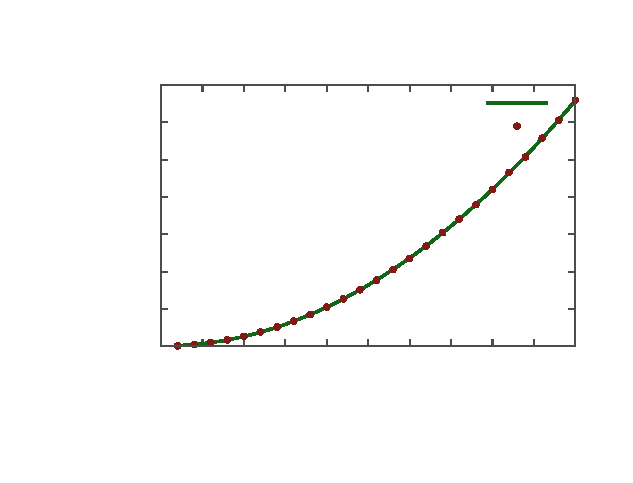
\includegraphics{./graficos/ajuste-seleccion}}%
    \gplfronttext
  \end{picture}%
\endgroup

	\end{center}
\end{frame}

\begin{frame}
    \vspace{2.5em}
    \textbf{Mergesort}
	\fontsize{5.8pt}{7.2}\selectfont
	\begin{center}
		% GNUPLOT: LaTeX picture with Postscript
\begingroup
  \makeatletter
  \providecommand\color[2][]{%
    \GenericError{(gnuplot) \space\space\space\@spaces}{%
      Package color not loaded in conjunction with
      terminal option `colourtext'%
    }{See the gnuplot documentation for explanation.%
    }{Either use 'blacktext' in gnuplot or load the package
      color.sty in LaTeX.}%
    \renewcommand\color[2][]{}%
  }%
  \providecommand\includegraphics[2][]{%
    \GenericError{(gnuplot) \space\space\space\@spaces}{%
      Package graphicx or graphics not loaded%
    }{See the gnuplot documentation for explanation.%
    }{The gnuplot epslatex terminal needs graphicx.sty or graphics.sty.}%
    \renewcommand\includegraphics[2][]{}%
  }%
  \providecommand\rotatebox[2]{#2}%
  \@ifundefined{ifGPcolor}{%
    \newif\ifGPcolor
    \GPcolortrue
  }{}%
  \@ifundefined{ifGPblacktext}{%
    \newif\ifGPblacktext
    \GPblacktextfalse
  }{}%
  % define a \g@addto@macro without @ in the name:
  \let\gplgaddtomacro\g@addto@macro
  % define empty templates for all commands taking text:
  \gdef\gplbacktext{}%
  \gdef\gplfronttext{}%
  \makeatother
  \ifGPblacktext
    % no textcolor at all
    \def\colorrgb#1{}%
    \def\colorgray#1{}%
  \else
    % gray or color?
    \ifGPcolor
      \def\colorrgb#1{\color[rgb]{#1}}%
      \def\colorgray#1{\color[gray]{#1}}%
      \expandafter\def\csname LTw\endcsname{\color{white}}%
      \expandafter\def\csname LTb\endcsname{\color{black}}%
      \expandafter\def\csname LTa\endcsname{\color{black}}%
      \expandafter\def\csname LT0\endcsname{\color[rgb]{1,0,0}}%
      \expandafter\def\csname LT1\endcsname{\color[rgb]{0,1,0}}%
      \expandafter\def\csname LT2\endcsname{\color[rgb]{0,0,1}}%
      \expandafter\def\csname LT3\endcsname{\color[rgb]{1,0,1}}%
      \expandafter\def\csname LT4\endcsname{\color[rgb]{0,1,1}}%
      \expandafter\def\csname LT5\endcsname{\color[rgb]{1,1,0}}%
      \expandafter\def\csname LT6\endcsname{\color[rgb]{0,0,0}}%
      \expandafter\def\csname LT7\endcsname{\color[rgb]{1,0.3,0}}%
      \expandafter\def\csname LT8\endcsname{\color[rgb]{0.5,0.5,0.5}}%
    \else
      % gray
      \def\colorrgb#1{\color{black}}%
      \def\colorgray#1{\color[gray]{#1}}%
      \expandafter\def\csname LTw\endcsname{\color{white}}%
      \expandafter\def\csname LTb\endcsname{\color{black}}%
      \expandafter\def\csname LTa\endcsname{\color{black}}%
      \expandafter\def\csname LT0\endcsname{\color{black}}%
      \expandafter\def\csname LT1\endcsname{\color{black}}%
      \expandafter\def\csname LT2\endcsname{\color{black}}%
      \expandafter\def\csname LT3\endcsname{\color{black}}%
      \expandafter\def\csname LT4\endcsname{\color{black}}%
      \expandafter\def\csname LT5\endcsname{\color{black}}%
      \expandafter\def\csname LT6\endcsname{\color{black}}%
      \expandafter\def\csname LT7\endcsname{\color{black}}%
      \expandafter\def\csname LT8\endcsname{\color{black}}%
    \fi
  \fi
    \setlength{\unitlength}{0.0500bp}%
    \ifx\gptboxheight\undefined%
      \newlength{\gptboxheight}%
      \newlength{\gptboxwidth}%
      \newsavebox{\gptboxtext}%
    \fi%
    \setlength{\fboxrule}{0.5pt}%
    \setlength{\fboxsep}{1pt}%
\begin{picture}(5760.00,4320.00)%
    \gplgaddtomacro\gplbacktext{%
      \colorrgb{0.30,0.30,0.30}%
      \put(1650,1246){\makebox(0,0)[r]{\strut{}$\textcolor{text}{0.0001}$}}%
      \colorrgb{0.30,0.30,0.30}%
      \put(1650,2050){\makebox(0,0)[r]{\strut{}$\textcolor{text}{0.001}$}}%
      \colorrgb{0.30,0.30,0.30}%
      \put(1650,2855){\makebox(0,0)[r]{\strut{}$\textcolor{text}{0.01}$}}%
      \colorrgb{0.30,0.30,0.30}%
      \put(1650,3659){\makebox(0,0)[r]{\strut{}$\textcolor{text}{0.1}$}}%
      \colorrgb{0.30,0.30,0.30}%
      \put(1782,1114){\rotatebox{45}{\makebox(0,0)[r]{\strut{}$\textcolor{text}{0}$}}}%
      \colorrgb{0.30,0.30,0.30}%
      \put(2230,1114){\rotatebox{45}{\makebox(0,0)[r]{\strut{}$\textcolor{text}{20000}$}}}%
      \colorrgb{0.30,0.30,0.30}%
      \put(2677,1114){\rotatebox{45}{\makebox(0,0)[r]{\strut{}$\textcolor{text}{40000}$}}}%
      \colorrgb{0.30,0.30,0.30}%
      \put(3125,1114){\rotatebox{45}{\makebox(0,0)[r]{\strut{}$\textcolor{text}{60000}$}}}%
      \colorrgb{0.30,0.30,0.30}%
      \put(3573,1114){\rotatebox{45}{\makebox(0,0)[r]{\strut{}$\textcolor{text}{80000}$}}}%
      \colorrgb{0.30,0.30,0.30}%
      \put(4020,1114){\rotatebox{45}{\makebox(0,0)[r]{\strut{}$\textcolor{text}{100000}$}}}%
      \colorrgb{0.30,0.30,0.30}%
      \put(4468,1114){\rotatebox{45}{\makebox(0,0)[r]{\strut{}$\textcolor{text}{120000}$}}}%
      \colorrgb{0.30,0.30,0.30}%
      \put(4915,1114){\rotatebox{45}{\makebox(0,0)[r]{\strut{}$\textcolor{text}{140000}$}}}%
      \colorrgb{0.30,0.30,0.30}%
      \put(5363,1114){\rotatebox{45}{\makebox(0,0)[r]{\strut{}$\textcolor{text}{160000}$}}}%
    }%
    \gplgaddtomacro\gplfronttext{%
      \colorrgb{0.30,0.30,0.30}%
      \put(220,2452){\rotatebox{-270}{\makebox(0,0){\strut{}Tiempo de ejecución (s)}}}%
      \colorrgb{0.30,0.30,0.30}%
      \put(3572,220){\makebox(0,0){\strut{}Tamaño del vector (elementos)}}%
      \colorrgb{0.30,0.30,0.30}%
      \put(3572,3989){\makebox(0,0){\strut{}Ajuste Mergesort}}%
      \csname LTb\endcsname%
      \put(4376,3486){\makebox(0,0)[r]{\strut{}Mergesort ajustado}}%
      \csname LTb\endcsname%
      \put(4376,3266){\makebox(0,0)[r]{\strut{}Mergesort}}%
    }%
    \gplbacktext
    \put(0,0){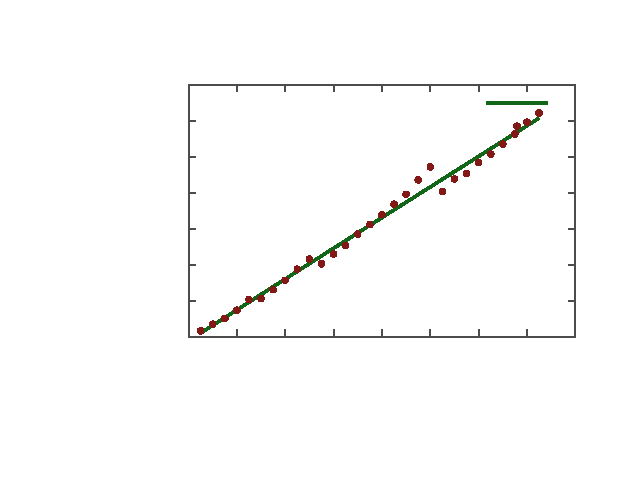
\includegraphics{./graficos/ajuste-mergesort}}%
    \gplfronttext
  \end{picture}%
\endgroup

	\end{center}
\end{frame}

\begin{frame}
    \vspace{2.5em}
    \textbf{Heapsort}
	\fontsize{5.8pt}{7.2}\selectfont
	\begin{center}
		% GNUPLOT: LaTeX picture with Postscript
\begingroup
  \makeatletter
  \providecommand\color[2][]{%
    \GenericError{(gnuplot) \space\space\space\@spaces}{%
      Package color not loaded in conjunction with
      terminal option `colourtext'%
    }{See the gnuplot documentation for explanation.%
    }{Either use 'blacktext' in gnuplot or load the package
      color.sty in LaTeX.}%
    \renewcommand\color[2][]{}%
  }%
  \providecommand\includegraphics[2][]{%
    \GenericError{(gnuplot) \space\space\space\@spaces}{%
      Package graphicx or graphics not loaded%
    }{See the gnuplot documentation for explanation.%
    }{The gnuplot epslatex terminal needs graphicx.sty or graphics.sty.}%
    \renewcommand\includegraphics[2][]{}%
  }%
  \providecommand\rotatebox[2]{#2}%
  \@ifundefined{ifGPcolor}{%
    \newif\ifGPcolor
    \GPcolortrue
  }{}%
  \@ifundefined{ifGPblacktext}{%
    \newif\ifGPblacktext
    \GPblacktextfalse
  }{}%
  % define a \g@addto@macro without @ in the name:
  \let\gplgaddtomacro\g@addto@macro
  % define empty templates for all commands taking text:
  \gdef\gplbacktext{}%
  \gdef\gplfronttext{}%
  \makeatother
  \ifGPblacktext
    % no textcolor at all
    \def\colorrgb#1{}%
    \def\colorgray#1{}%
  \else
    % gray or color?
    \ifGPcolor
      \def\colorrgb#1{\color[rgb]{#1}}%
      \def\colorgray#1{\color[gray]{#1}}%
      \expandafter\def\csname LTw\endcsname{\color{white}}%
      \expandafter\def\csname LTb\endcsname{\color{black}}%
      \expandafter\def\csname LTa\endcsname{\color{black}}%
      \expandafter\def\csname LT0\endcsname{\color[rgb]{1,0,0}}%
      \expandafter\def\csname LT1\endcsname{\color[rgb]{0,1,0}}%
      \expandafter\def\csname LT2\endcsname{\color[rgb]{0,0,1}}%
      \expandafter\def\csname LT3\endcsname{\color[rgb]{1,0,1}}%
      \expandafter\def\csname LT4\endcsname{\color[rgb]{0,1,1}}%
      \expandafter\def\csname LT5\endcsname{\color[rgb]{1,1,0}}%
      \expandafter\def\csname LT6\endcsname{\color[rgb]{0,0,0}}%
      \expandafter\def\csname LT7\endcsname{\color[rgb]{1,0.3,0}}%
      \expandafter\def\csname LT8\endcsname{\color[rgb]{0.5,0.5,0.5}}%
    \else
      % gray
      \def\colorrgb#1{\color{black}}%
      \def\colorgray#1{\color[gray]{#1}}%
      \expandafter\def\csname LTw\endcsname{\color{white}}%
      \expandafter\def\csname LTb\endcsname{\color{black}}%
      \expandafter\def\csname LTa\endcsname{\color{black}}%
      \expandafter\def\csname LT0\endcsname{\color{black}}%
      \expandafter\def\csname LT1\endcsname{\color{black}}%
      \expandafter\def\csname LT2\endcsname{\color{black}}%
      \expandafter\def\csname LT3\endcsname{\color{black}}%
      \expandafter\def\csname LT4\endcsname{\color{black}}%
      \expandafter\def\csname LT5\endcsname{\color{black}}%
      \expandafter\def\csname LT6\endcsname{\color{black}}%
      \expandafter\def\csname LT7\endcsname{\color{black}}%
      \expandafter\def\csname LT8\endcsname{\color{black}}%
    \fi
  \fi
    \setlength{\unitlength}{0.0500bp}%
    \ifx\gptboxheight\undefined%
      \newlength{\gptboxheight}%
      \newlength{\gptboxwidth}%
      \newsavebox{\gptboxtext}%
    \fi%
    \setlength{\fboxrule}{0.5pt}%
    \setlength{\fboxsep}{1pt}%
\begin{picture}(5760.00,4320.00)%
    \gplgaddtomacro\gplbacktext{%
      \colorrgb{0.30,0.30,0.30}%
      \put(1518,1246){\makebox(0,0)[r]{\strut{}$\textcolor{text}{0}$}}%
      \colorrgb{0.30,0.30,0.30}%
      \put(1518,1591){\makebox(0,0)[r]{\strut{}$\textcolor{text}{0.005}$}}%
      \colorrgb{0.30,0.30,0.30}%
      \put(1518,1935){\makebox(0,0)[r]{\strut{}$\textcolor{text}{0.01}$}}%
      \colorrgb{0.30,0.30,0.30}%
      \put(1518,2280){\makebox(0,0)[r]{\strut{}$\textcolor{text}{0.015}$}}%
      \colorrgb{0.30,0.30,0.30}%
      \put(1518,2625){\makebox(0,0)[r]{\strut{}$\textcolor{text}{0.02}$}}%
      \colorrgb{0.30,0.30,0.30}%
      \put(1518,2970){\makebox(0,0)[r]{\strut{}$\textcolor{text}{0.025}$}}%
      \colorrgb{0.30,0.30,0.30}%
      \put(1518,3314){\makebox(0,0)[r]{\strut{}$\textcolor{text}{0.03}$}}%
      \colorrgb{0.30,0.30,0.30}%
      \put(1518,3659){\makebox(0,0)[r]{\strut{}$\textcolor{text}{0.035}$}}%
      \colorrgb{0.30,0.30,0.30}%
      \put(1650,1114){\rotatebox{45}{\makebox(0,0)[r]{\strut{}$\textcolor{text}{0}$}}}%
      \colorrgb{0.30,0.30,0.30}%
      \put(2114,1114){\rotatebox{45}{\makebox(0,0)[r]{\strut{}$\textcolor{text}{20000}$}}}%
      \colorrgb{0.30,0.30,0.30}%
      \put(2578,1114){\rotatebox{45}{\makebox(0,0)[r]{\strut{}$\textcolor{text}{40000}$}}}%
      \colorrgb{0.30,0.30,0.30}%
      \put(3042,1114){\rotatebox{45}{\makebox(0,0)[r]{\strut{}$\textcolor{text}{60000}$}}}%
      \colorrgb{0.30,0.30,0.30}%
      \put(3507,1114){\rotatebox{45}{\makebox(0,0)[r]{\strut{}$\textcolor{text}{80000}$}}}%
      \colorrgb{0.30,0.30,0.30}%
      \put(3971,1114){\rotatebox{45}{\makebox(0,0)[r]{\strut{}$\textcolor{text}{100000}$}}}%
      \colorrgb{0.30,0.30,0.30}%
      \put(4435,1114){\rotatebox{45}{\makebox(0,0)[r]{\strut{}$\textcolor{text}{120000}$}}}%
      \colorrgb{0.30,0.30,0.30}%
      \put(4899,1114){\rotatebox{45}{\makebox(0,0)[r]{\strut{}$\textcolor{text}{140000}$}}}%
      \colorrgb{0.30,0.30,0.30}%
      \put(5363,1114){\rotatebox{45}{\makebox(0,0)[r]{\strut{}$\textcolor{text}{160000}$}}}%
    }%
    \gplgaddtomacro\gplfronttext{%
      \colorrgb{0.30,0.30,0.30}%
      \put(220,2452){\rotatebox{-270}{\makebox(0,0){\strut{}Tiempo de ejecución (s)}}}%
      \colorrgb{0.30,0.30,0.30}%
      \put(3506,220){\makebox(0,0){\strut{}Tamaño del vector (elementos)}}%
      \colorrgb{0.30,0.30,0.30}%
      \put(3506,3989){\makebox(0,0){\strut{}Ajuste Heapsort}}%
      \csname LTb\endcsname%
      \put(4376,3486){\makebox(0,0)[r]{\strut{}1.20e-11$ \cdot x^{7.04e-01}+x \cdot 1.60e-07$}}%
      \csname LTb\endcsname%
      \put(4376,3266){\makebox(0,0)[r]{\strut{}Heapsort}}%
    }%
    \gplbacktext
    \put(0,0){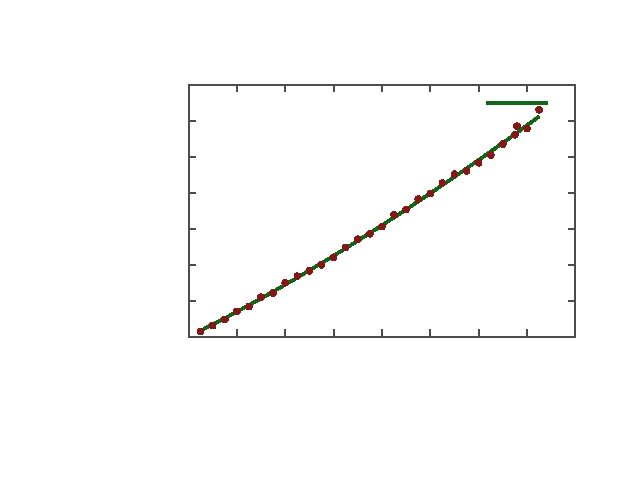
\includegraphics{./graficos/ajuste-heapsort}}%
    \gplfronttext
  \end{picture}%
\endgroup

	\end{center}
\end{frame}

\begin{frame}
    \vspace{2.5em}
    \textbf{Quicksort}
	\fontsize{5.8pt}{7.2}\selectfont
	\begin{center}
		% GNUPLOT: LaTeX picture with Postscript
\begingroup
  \makeatletter
  \providecommand\color[2][]{%
    \GenericError{(gnuplot) \space\space\space\@spaces}{%
      Package color not loaded in conjunction with
      terminal option `colourtext'%
    }{See the gnuplot documentation for explanation.%
    }{Either use 'blacktext' in gnuplot or load the package
      color.sty in LaTeX.}%
    \renewcommand\color[2][]{}%
  }%
  \providecommand\includegraphics[2][]{%
    \GenericError{(gnuplot) \space\space\space\@spaces}{%
      Package graphicx or graphics not loaded%
    }{See the gnuplot documentation for explanation.%
    }{The gnuplot epslatex terminal needs graphicx.sty or graphics.sty.}%
    \renewcommand\includegraphics[2][]{}%
  }%
  \providecommand\rotatebox[2]{#2}%
  \@ifundefined{ifGPcolor}{%
    \newif\ifGPcolor
    \GPcolortrue
  }{}%
  \@ifundefined{ifGPblacktext}{%
    \newif\ifGPblacktext
    \GPblacktextfalse
  }{}%
  % define a \g@addto@macro without @ in the name:
  \let\gplgaddtomacro\g@addto@macro
  % define empty templates for all commands taking text:
  \gdef\gplbacktext{}%
  \gdef\gplfronttext{}%
  \makeatother
  \ifGPblacktext
    % no textcolor at all
    \def\colorrgb#1{}%
    \def\colorgray#1{}%
  \else
    % gray or color?
    \ifGPcolor
      \def\colorrgb#1{\color[rgb]{#1}}%
      \def\colorgray#1{\color[gray]{#1}}%
      \expandafter\def\csname LTw\endcsname{\color{white}}%
      \expandafter\def\csname LTb\endcsname{\color{black}}%
      \expandafter\def\csname LTa\endcsname{\color{black}}%
      \expandafter\def\csname LT0\endcsname{\color[rgb]{1,0,0}}%
      \expandafter\def\csname LT1\endcsname{\color[rgb]{0,1,0}}%
      \expandafter\def\csname LT2\endcsname{\color[rgb]{0,0,1}}%
      \expandafter\def\csname LT3\endcsname{\color[rgb]{1,0,1}}%
      \expandafter\def\csname LT4\endcsname{\color[rgb]{0,1,1}}%
      \expandafter\def\csname LT5\endcsname{\color[rgb]{1,1,0}}%
      \expandafter\def\csname LT6\endcsname{\color[rgb]{0,0,0}}%
      \expandafter\def\csname LT7\endcsname{\color[rgb]{1,0.3,0}}%
      \expandafter\def\csname LT8\endcsname{\color[rgb]{0.5,0.5,0.5}}%
    \else
      % gray
      \def\colorrgb#1{\color{black}}%
      \def\colorgray#1{\color[gray]{#1}}%
      \expandafter\def\csname LTw\endcsname{\color{white}}%
      \expandafter\def\csname LTb\endcsname{\color{black}}%
      \expandafter\def\csname LTa\endcsname{\color{black}}%
      \expandafter\def\csname LT0\endcsname{\color{black}}%
      \expandafter\def\csname LT1\endcsname{\color{black}}%
      \expandafter\def\csname LT2\endcsname{\color{black}}%
      \expandafter\def\csname LT3\endcsname{\color{black}}%
      \expandafter\def\csname LT4\endcsname{\color{black}}%
      \expandafter\def\csname LT5\endcsname{\color{black}}%
      \expandafter\def\csname LT6\endcsname{\color{black}}%
      \expandafter\def\csname LT7\endcsname{\color{black}}%
      \expandafter\def\csname LT8\endcsname{\color{black}}%
    \fi
  \fi
    \setlength{\unitlength}{0.0500bp}%
    \ifx\gptboxheight\undefined%
      \newlength{\gptboxheight}%
      \newlength{\gptboxwidth}%
      \newsavebox{\gptboxtext}%
    \fi%
    \setlength{\fboxrule}{0.5pt}%
    \setlength{\fboxsep}{1pt}%
\begin{picture}(5760.00,4320.00)%
    \gplgaddtomacro\gplbacktext{%
      \colorrgb{0.30,0.30,0.30}%
      \put(1518,1246){\makebox(0,0)[r]{\strut{}$\textcolor{text}{0}$}}%
      \colorrgb{0.30,0.30,0.30}%
      \put(1518,1729){\makebox(0,0)[r]{\strut{}$\textcolor{text}{0.005}$}}%
      \colorrgb{0.30,0.30,0.30}%
      \put(1518,2211){\makebox(0,0)[r]{\strut{}$\textcolor{text}{0.01}$}}%
      \colorrgb{0.30,0.30,0.30}%
      \put(1518,2694){\makebox(0,0)[r]{\strut{}$\textcolor{text}{0.015}$}}%
      \colorrgb{0.30,0.30,0.30}%
      \put(1518,3176){\makebox(0,0)[r]{\strut{}$\textcolor{text}{0.02}$}}%
      \colorrgb{0.30,0.30,0.30}%
      \put(1518,3659){\makebox(0,0)[r]{\strut{}$\textcolor{text}{0.025}$}}%
      \colorrgb{0.30,0.30,0.30}%
      \put(1650,1114){\rotatebox{45}{\makebox(0,0)[r]{\strut{}$\textcolor{text}{0}$}}}%
      \colorrgb{0.30,0.30,0.30}%
      \put(2114,1114){\rotatebox{45}{\makebox(0,0)[r]{\strut{}$\textcolor{text}{20000}$}}}%
      \colorrgb{0.30,0.30,0.30}%
      \put(2578,1114){\rotatebox{45}{\makebox(0,0)[r]{\strut{}$\textcolor{text}{40000}$}}}%
      \colorrgb{0.30,0.30,0.30}%
      \put(3042,1114){\rotatebox{45}{\makebox(0,0)[r]{\strut{}$\textcolor{text}{60000}$}}}%
      \colorrgb{0.30,0.30,0.30}%
      \put(3507,1114){\rotatebox{45}{\makebox(0,0)[r]{\strut{}$\textcolor{text}{80000}$}}}%
      \colorrgb{0.30,0.30,0.30}%
      \put(3971,1114){\rotatebox{45}{\makebox(0,0)[r]{\strut{}$\textcolor{text}{100000}$}}}%
      \colorrgb{0.30,0.30,0.30}%
      \put(4435,1114){\rotatebox{45}{\makebox(0,0)[r]{\strut{}$\textcolor{text}{120000}$}}}%
      \colorrgb{0.30,0.30,0.30}%
      \put(4899,1114){\rotatebox{45}{\makebox(0,0)[r]{\strut{}$\textcolor{text}{140000}$}}}%
      \colorrgb{0.30,0.30,0.30}%
      \put(5363,1114){\rotatebox{45}{\makebox(0,0)[r]{\strut{}$\textcolor{text}{160000}$}}}%
    }%
    \gplgaddtomacro\gplfronttext{%
      \colorrgb{0.30,0.30,0.30}%
      \put(220,2452){\rotatebox{-270}{\makebox(0,0){\strut{}Tiempo de ejecución (s)}}}%
      \colorrgb{0.30,0.30,0.30}%
      \put(3506,220){\makebox(0,0){\strut{}Tamaño del vector (elementos)}}%
      \colorrgb{0.30,0.30,0.30}%
      \put(3506,3989){\makebox(0,0){\strut{}Ajuste Quicksort}}%
      \csname LTb\endcsname%
      \put(4376,3486){\makebox(0,0)[r]{\strut{}$ 1.14e-08 \cdot x\log x + 7.66e-09 x + 4.91e-06$}}%
      \csname LTb\endcsname%
      \put(4376,3266){\makebox(0,0)[r]{\strut{}Quicksort}}%
    }%
    \gplbacktext
    \put(0,0){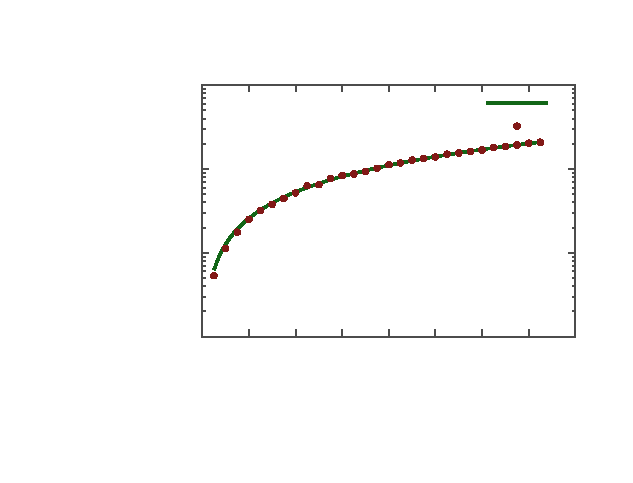
\includegraphics{./graficos/ajuste-quicksort}}%
    \gplfronttext
  \end{picture}%
\endgroup

	\end{center}
\end{frame}

\begin{frame}
    \vspace{2.5em}
    \textbf{Floyd}
	\fontsize{7pt}{7.2}\selectfont
	\begin{center}
		% GNUPLOT: LaTeX picture with Postscript
\begingroup
  \makeatletter
  \providecommand\color[2][]{%
    \GenericError{(gnuplot) \space\space\space\@spaces}{%
      Package color not loaded in conjunction with
      terminal option `colourtext'%
    }{See the gnuplot documentation for explanation.%
    }{Either use 'blacktext' in gnuplot or load the package
      color.sty in LaTeX.}%
    \renewcommand\color[2][]{}%
  }%
  \providecommand\includegraphics[2][]{%
    \GenericError{(gnuplot) \space\space\space\@spaces}{%
      Package graphicx or graphics not loaded%
    }{See the gnuplot documentation for explanation.%
    }{The gnuplot epslatex terminal needs graphicx.sty or graphics.sty.}%
    \renewcommand\includegraphics[2][]{}%
  }%
  \providecommand\rotatebox[2]{#2}%
  \@ifundefined{ifGPcolor}{%
    \newif\ifGPcolor
    \GPcolortrue
  }{}%
  \@ifundefined{ifGPblacktext}{%
    \newif\ifGPblacktext
    \GPblacktextfalse
  }{}%
  % define a \g@addto@macro without @ in the name:
  \let\gplgaddtomacro\g@addto@macro
  % define empty templates for all commands taking text:
  \gdef\gplbacktext{}%
  \gdef\gplfronttext{}%
  \makeatother
  \ifGPblacktext
    % no textcolor at all
    \def\colorrgb#1{}%
    \def\colorgray#1{}%
  \else
    % gray or color?
    \ifGPcolor
      \def\colorrgb#1{\color[rgb]{#1}}%
      \def\colorgray#1{\color[gray]{#1}}%
      \expandafter\def\csname LTw\endcsname{\color{white}}%
      \expandafter\def\csname LTb\endcsname{\color{black}}%
      \expandafter\def\csname LTa\endcsname{\color{black}}%
      \expandafter\def\csname LT0\endcsname{\color[rgb]{1,0,0}}%
      \expandafter\def\csname LT1\endcsname{\color[rgb]{0,1,0}}%
      \expandafter\def\csname LT2\endcsname{\color[rgb]{0,0,1}}%
      \expandafter\def\csname LT3\endcsname{\color[rgb]{1,0,1}}%
      \expandafter\def\csname LT4\endcsname{\color[rgb]{0,1,1}}%
      \expandafter\def\csname LT5\endcsname{\color[rgb]{1,1,0}}%
      \expandafter\def\csname LT6\endcsname{\color[rgb]{0,0,0}}%
      \expandafter\def\csname LT7\endcsname{\color[rgb]{1,0.3,0}}%
      \expandafter\def\csname LT8\endcsname{\color[rgb]{0.5,0.5,0.5}}%
    \else
      % gray
      \def\colorrgb#1{\color{black}}%
      \def\colorgray#1{\color[gray]{#1}}%
      \expandafter\def\csname LTw\endcsname{\color{white}}%
      \expandafter\def\csname LTb\endcsname{\color{black}}%
      \expandafter\def\csname LTa\endcsname{\color{black}}%
      \expandafter\def\csname LT0\endcsname{\color{black}}%
      \expandafter\def\csname LT1\endcsname{\color{black}}%
      \expandafter\def\csname LT2\endcsname{\color{black}}%
      \expandafter\def\csname LT3\endcsname{\color{black}}%
      \expandafter\def\csname LT4\endcsname{\color{black}}%
      \expandafter\def\csname LT5\endcsname{\color{black}}%
      \expandafter\def\csname LT6\endcsname{\color{black}}%
      \expandafter\def\csname LT7\endcsname{\color{black}}%
      \expandafter\def\csname LT8\endcsname{\color{black}}%
    \fi
  \fi
    \setlength{\unitlength}{0.0500bp}%
    \ifx\gptboxheight\undefined%
      \newlength{\gptboxheight}%
      \newlength{\gptboxwidth}%
      \newsavebox{\gptboxtext}%
    \fi%
    \setlength{\fboxrule}{0.5pt}%
    \setlength{\fboxsep}{1pt}%
\begin{picture}(5760.00,4320.00)%
    \gplgaddtomacro\gplbacktext{%
      \colorrgb{0.30,0.30,0.30}%
      \put(1122,1060){\makebox(0,0)[r]{\strut{}$\textcolor{text}{0}$}}%
      \colorrgb{0.30,0.30,0.30}%
      \put(1122,1349){\makebox(0,0)[r]{\strut{}$\textcolor{text}{2}$}}%
      \colorrgb{0.30,0.30,0.30}%
      \put(1122,1638){\makebox(0,0)[r]{\strut{}$\textcolor{text}{4}$}}%
      \colorrgb{0.30,0.30,0.30}%
      \put(1122,1926){\makebox(0,0)[r]{\strut{}$\textcolor{text}{6}$}}%
      \colorrgb{0.30,0.30,0.30}%
      \put(1122,2215){\makebox(0,0)[r]{\strut{}$\textcolor{text}{8}$}}%
      \colorrgb{0.30,0.30,0.30}%
      \put(1122,2504){\makebox(0,0)[r]{\strut{}$\textcolor{text}{10}$}}%
      \colorrgb{0.30,0.30,0.30}%
      \put(1122,2793){\makebox(0,0)[r]{\strut{}$\textcolor{text}{12}$}}%
      \colorrgb{0.30,0.30,0.30}%
      \put(1122,3081){\makebox(0,0)[r]{\strut{}$\textcolor{text}{14}$}}%
      \colorrgb{0.30,0.30,0.30}%
      \put(1122,3370){\makebox(0,0)[r]{\strut{}$\textcolor{text}{16}$}}%
      \colorrgb{0.30,0.30,0.30}%
      \put(1122,3659){\makebox(0,0)[r]{\strut{}$\textcolor{text}{18}$}}%
      \colorrgb{0.30,0.30,0.30}%
      \put(1254,928){\rotatebox{45}{\makebox(0,0)[r]{\strut{}$\textcolor{text}{0}$}}}%
      \colorrgb{0.30,0.30,0.30}%
      \put(1768,928){\rotatebox{45}{\makebox(0,0)[r]{\strut{}$\textcolor{text}{200}$}}}%
      \colorrgb{0.30,0.30,0.30}%
      \put(2281,928){\rotatebox{45}{\makebox(0,0)[r]{\strut{}$\textcolor{text}{400}$}}}%
      \colorrgb{0.30,0.30,0.30}%
      \put(2795,928){\rotatebox{45}{\makebox(0,0)[r]{\strut{}$\textcolor{text}{600}$}}}%
      \colorrgb{0.30,0.30,0.30}%
      \put(3309,928){\rotatebox{45}{\makebox(0,0)[r]{\strut{}$\textcolor{text}{800}$}}}%
      \colorrgb{0.30,0.30,0.30}%
      \put(3822,928){\rotatebox{45}{\makebox(0,0)[r]{\strut{}$\textcolor{text}{1000}$}}}%
      \colorrgb{0.30,0.30,0.30}%
      \put(4336,928){\rotatebox{45}{\makebox(0,0)[r]{\strut{}$\textcolor{text}{1200}$}}}%
      \colorrgb{0.30,0.30,0.30}%
      \put(4849,928){\rotatebox{45}{\makebox(0,0)[r]{\strut{}$\textcolor{text}{1400}$}}}%
      \colorrgb{0.30,0.30,0.30}%
      \put(5363,928){\rotatebox{45}{\makebox(0,0)[r]{\strut{}$\textcolor{text}{1600}$}}}%
    }%
    \gplgaddtomacro\gplfronttext{%
      \colorrgb{0.30,0.30,0.30}%
      \put(220,2359){\rotatebox{-270}{\makebox(0,0){\strut{}Tiempo de ejecución (s)}}}%
      \colorrgb{0.30,0.30,0.30}%
      \put(3308,220){\makebox(0,0){\strut{}Tamaño del vector (elementos)}}%
      \colorrgb{0.30,0.30,0.30}%
      \put(3308,3989){\makebox(0,0){\strut{}Ajuste Floyd}}%
      \csname LTb\endcsname%
      \put(4376,3486){\makebox(0,0)[r]{\strut{}5.38e-09$x^3$+4.48e-07$x^2$+-2.70e-04$x$+3.11e-02}}%
      \csname LTb\endcsname%
      \put(4376,3266){\makebox(0,0)[r]{\strut{}Floyd}}%
    }%
    \gplbacktext
    \put(0,0){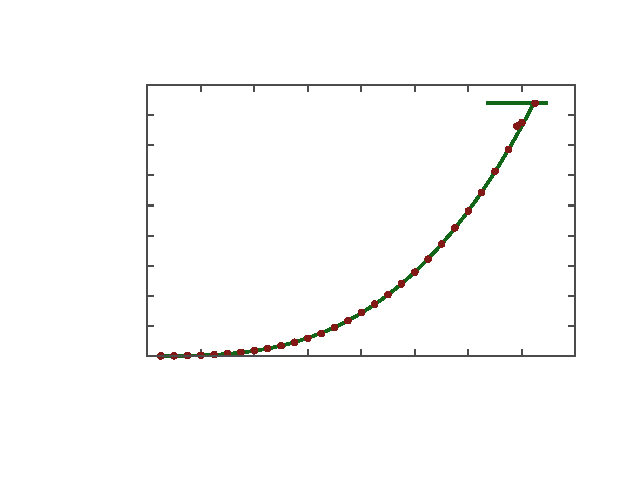
\includegraphics{./graficos/ajuste-floyd}}%
    \gplfronttext
  \end{picture}%
\endgroup

	\end{center}
\end{frame}

\begin{frame}
    \vspace{2.5em}
    \textbf{Hanoi}
	\fontsize{8pt}{7.2}\selectfont
	\begin{center}
		% GNUPLOT: LaTeX picture with Postscript
\begingroup
  \makeatletter
  \providecommand\color[2][]{%
    \GenericError{(gnuplot) \space\space\space\@spaces}{%
      Package color not loaded in conjunction with
      terminal option `colourtext'%
    }{See the gnuplot documentation for explanation.%
    }{Either use 'blacktext' in gnuplot or load the package
      color.sty in LaTeX.}%
    \renewcommand\color[2][]{}%
  }%
  \providecommand\includegraphics[2][]{%
    \GenericError{(gnuplot) \space\space\space\@spaces}{%
      Package graphicx or graphics not loaded%
    }{See the gnuplot documentation for explanation.%
    }{The gnuplot epslatex terminal needs graphicx.sty or graphics.sty.}%
    \renewcommand\includegraphics[2][]{}%
  }%
  \providecommand\rotatebox[2]{#2}%
  \@ifundefined{ifGPcolor}{%
    \newif\ifGPcolor
    \GPcolortrue
  }{}%
  \@ifundefined{ifGPblacktext}{%
    \newif\ifGPblacktext
    \GPblacktextfalse
  }{}%
  % define a \g@addto@macro without @ in the name:
  \let\gplgaddtomacro\g@addto@macro
  % define empty templates for all commands taking text:
  \gdef\gplbacktext{}%
  \gdef\gplfronttext{}%
  \makeatother
  \ifGPblacktext
    % no textcolor at all
    \def\colorrgb#1{}%
    \def\colorgray#1{}%
  \else
    % gray or color?
    \ifGPcolor
      \def\colorrgb#1{\color[rgb]{#1}}%
      \def\colorgray#1{\color[gray]{#1}}%
      \expandafter\def\csname LTw\endcsname{\color{white}}%
      \expandafter\def\csname LTb\endcsname{\color{black}}%
      \expandafter\def\csname LTa\endcsname{\color{black}}%
      \expandafter\def\csname LT0\endcsname{\color[rgb]{1,0,0}}%
      \expandafter\def\csname LT1\endcsname{\color[rgb]{0,1,0}}%
      \expandafter\def\csname LT2\endcsname{\color[rgb]{0,0,1}}%
      \expandafter\def\csname LT3\endcsname{\color[rgb]{1,0,1}}%
      \expandafter\def\csname LT4\endcsname{\color[rgb]{0,1,1}}%
      \expandafter\def\csname LT5\endcsname{\color[rgb]{1,1,0}}%
      \expandafter\def\csname LT6\endcsname{\color[rgb]{0,0,0}}%
      \expandafter\def\csname LT7\endcsname{\color[rgb]{1,0.3,0}}%
      \expandafter\def\csname LT8\endcsname{\color[rgb]{0.5,0.5,0.5}}%
    \else
      % gray
      \def\colorrgb#1{\color{black}}%
      \def\colorgray#1{\color[gray]{#1}}%
      \expandafter\def\csname LTw\endcsname{\color{white}}%
      \expandafter\def\csname LTb\endcsname{\color{black}}%
      \expandafter\def\csname LTa\endcsname{\color{black}}%
      \expandafter\def\csname LT0\endcsname{\color{black}}%
      \expandafter\def\csname LT1\endcsname{\color{black}}%
      \expandafter\def\csname LT2\endcsname{\color{black}}%
      \expandafter\def\csname LT3\endcsname{\color{black}}%
      \expandafter\def\csname LT4\endcsname{\color{black}}%
      \expandafter\def\csname LT5\endcsname{\color{black}}%
      \expandafter\def\csname LT6\endcsname{\color{black}}%
      \expandafter\def\csname LT7\endcsname{\color{black}}%
      \expandafter\def\csname LT8\endcsname{\color{black}}%
    \fi
  \fi
    \setlength{\unitlength}{0.0500bp}%
    \ifx\gptboxheight\undefined%
      \newlength{\gptboxheight}%
      \newlength{\gptboxwidth}%
      \newsavebox{\gptboxtext}%
    \fi%
    \setlength{\fboxrule}{0.5pt}%
    \setlength{\fboxsep}{1pt}%
\begin{picture}(5760.00,4320.00)%
    \gplgaddtomacro\gplbacktext{%
      \colorrgb{0.30,0.30,0.30}%
      \put(990,873){\makebox(0,0)[r]{\strut{}$\textcolor{text}{0}$}}%
      \colorrgb{0.30,0.30,0.30}%
      \put(990,1271){\makebox(0,0)[r]{\strut{}$\textcolor{text}{1}$}}%
      \colorrgb{0.30,0.30,0.30}%
      \put(990,1669){\makebox(0,0)[r]{\strut{}$\textcolor{text}{2}$}}%
      \colorrgb{0.30,0.30,0.30}%
      \put(990,2067){\makebox(0,0)[r]{\strut{}$\textcolor{text}{3}$}}%
      \colorrgb{0.30,0.30,0.30}%
      \put(990,2465){\makebox(0,0)[r]{\strut{}$\textcolor{text}{4}$}}%
      \colorrgb{0.30,0.30,0.30}%
      \put(990,2863){\makebox(0,0)[r]{\strut{}$\textcolor{text}{5}$}}%
      \colorrgb{0.30,0.30,0.30}%
      \put(990,3261){\makebox(0,0)[r]{\strut{}$\textcolor{text}{6}$}}%
      \colorrgb{0.30,0.30,0.30}%
      \put(990,3659){\makebox(0,0)[r]{\strut{}$\textcolor{text}{7}$}}%
      \colorrgb{0.30,0.30,0.30}%
      \put(1122,741){\rotatebox{45}{\makebox(0,0)[r]{\strut{}$\textcolor{text}{5}$}}}%
      \colorrgb{0.30,0.30,0.30}%
      \put(1970,741){\rotatebox{45}{\makebox(0,0)[r]{\strut{}$\textcolor{text}{10}$}}}%
      \colorrgb{0.30,0.30,0.30}%
      \put(2818,741){\rotatebox{45}{\makebox(0,0)[r]{\strut{}$\textcolor{text}{15}$}}}%
      \colorrgb{0.30,0.30,0.30}%
      \put(3667,741){\rotatebox{45}{\makebox(0,0)[r]{\strut{}$\textcolor{text}{20}$}}}%
      \colorrgb{0.30,0.30,0.30}%
      \put(4515,741){\rotatebox{45}{\makebox(0,0)[r]{\strut{}$\textcolor{text}{25}$}}}%
      \colorrgb{0.30,0.30,0.30}%
      \put(5363,741){\rotatebox{45}{\makebox(0,0)[r]{\strut{}$\textcolor{text}{30}$}}}%
    }%
    \gplgaddtomacro\gplfronttext{%
      \colorrgb{0.30,0.30,0.30}%
      \put(220,2266){\rotatebox{-270}{\makebox(0,0){\strut{}Tiempo de ejecución (s)}}}%
      \colorrgb{0.30,0.30,0.30}%
      \put(3242,220){\makebox(0,0){\strut{}Tamaño del vector (elementos)}}%
      \colorrgb{0.30,0.30,0.30}%
      \put(3242,3989){\makebox(0,0){\strut{}Ajuste hanoi}}%
      \csname LTb\endcsname%
      \put(4376,3486){\makebox(0,0)[r]{\strut{}Hanoi ajustado}}%
      \csname LTb\endcsname%
      \put(4376,3266){\makebox(0,0)[r]{\strut{}Hanoi}}%
    }%
    \gplbacktext
    \put(0,0){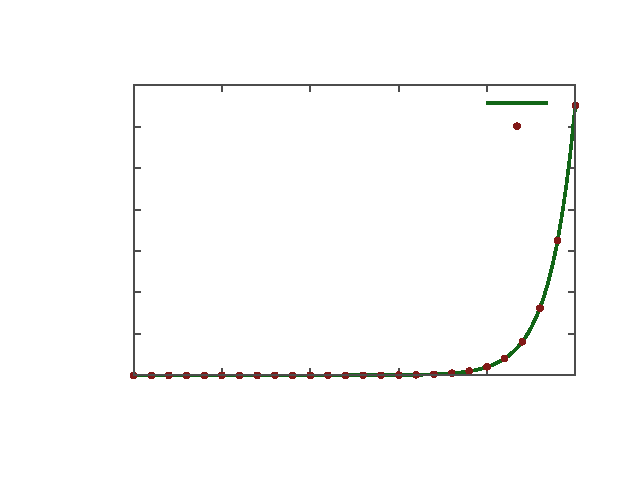
\includegraphics{./graficos/ajuste-hanoi}}%
    \gplfronttext
  \end{picture}%
\endgroup

	\end{center}
\end{frame}

\begin{frame}{Ajustes con otras funciones}
	Veamos por último lo que ocurre si intentamos ajustar los datos recogidos experimentalmente a una función que no coincide con la eficiencia teórica del algoritmo.
\end{frame}

\begin{frame}{Burbuja con función logarítmica}
	\fontsize{8pt}{7.2}\selectfont
	\begin{center}
		% GNUPLOT: LaTeX picture with Postscript
\begingroup
  \makeatletter
  \providecommand\color[2][]{%
    \GenericError{(gnuplot) \space\space\space\@spaces}{%
      Package color not loaded in conjunction with
      terminal option `colourtext'%
    }{See the gnuplot documentation for explanation.%
    }{Either use 'blacktext' in gnuplot or load the package
      color.sty in LaTeX.}%
    \renewcommand\color[2][]{}%
  }%
  \providecommand\includegraphics[2][]{%
    \GenericError{(gnuplot) \space\space\space\@spaces}{%
      Package graphicx or graphics not loaded%
    }{See the gnuplot documentation for explanation.%
    }{The gnuplot epslatex terminal needs graphicx.sty or graphics.sty.}%
    \renewcommand\includegraphics[2][]{}%
  }%
  \providecommand\rotatebox[2]{#2}%
  \@ifundefined{ifGPcolor}{%
    \newif\ifGPcolor
    \GPcolortrue
  }{}%
  \@ifundefined{ifGPblacktext}{%
    \newif\ifGPblacktext
    \GPblacktextfalse
  }{}%
  % define a \g@addto@macro without @ in the name:
  \let\gplgaddtomacro\g@addto@macro
  % define empty templates for all commands taking text:
  \gdef\gplbacktext{}%
  \gdef\gplfronttext{}%
  \makeatother
  \ifGPblacktext
    % no textcolor at all
    \def\colorrgb#1{}%
    \def\colorgray#1{}%
  \else
    % gray or color?
    \ifGPcolor
      \def\colorrgb#1{\color[rgb]{#1}}%
      \def\colorgray#1{\color[gray]{#1}}%
      \expandafter\def\csname LTw\endcsname{\color{white}}%
      \expandafter\def\csname LTb\endcsname{\color{black}}%
      \expandafter\def\csname LTa\endcsname{\color{black}}%
      \expandafter\def\csname LT0\endcsname{\color[rgb]{1,0,0}}%
      \expandafter\def\csname LT1\endcsname{\color[rgb]{0,1,0}}%
      \expandafter\def\csname LT2\endcsname{\color[rgb]{0,0,1}}%
      \expandafter\def\csname LT3\endcsname{\color[rgb]{1,0,1}}%
      \expandafter\def\csname LT4\endcsname{\color[rgb]{0,1,1}}%
      \expandafter\def\csname LT5\endcsname{\color[rgb]{1,1,0}}%
      \expandafter\def\csname LT6\endcsname{\color[rgb]{0,0,0}}%
      \expandafter\def\csname LT7\endcsname{\color[rgb]{1,0.3,0}}%
      \expandafter\def\csname LT8\endcsname{\color[rgb]{0.5,0.5,0.5}}%
    \else
      % gray
      \def\colorrgb#1{\color{black}}%
      \def\colorgray#1{\color[gray]{#1}}%
      \expandafter\def\csname LTw\endcsname{\color{white}}%
      \expandafter\def\csname LTb\endcsname{\color{black}}%
      \expandafter\def\csname LTa\endcsname{\color{black}}%
      \expandafter\def\csname LT0\endcsname{\color{black}}%
      \expandafter\def\csname LT1\endcsname{\color{black}}%
      \expandafter\def\csname LT2\endcsname{\color{black}}%
      \expandafter\def\csname LT3\endcsname{\color{black}}%
      \expandafter\def\csname LT4\endcsname{\color{black}}%
      \expandafter\def\csname LT5\endcsname{\color{black}}%
      \expandafter\def\csname LT6\endcsname{\color{black}}%
      \expandafter\def\csname LT7\endcsname{\color{black}}%
      \expandafter\def\csname LT8\endcsname{\color{black}}%
    \fi
  \fi
    \setlength{\unitlength}{0.0500bp}%
    \ifx\gptboxheight\undefined%
      \newlength{\gptboxheight}%
      \newlength{\gptboxwidth}%
      \newsavebox{\gptboxtext}%
    \fi%
    \setlength{\fboxrule}{0.5pt}%
    \setlength{\fboxsep}{1pt}%
\begin{picture}(5760.00,4320.00)%
    \gplgaddtomacro\gplbacktext{%
      \colorrgb{0.30,0.30,0.30}%
      \put(1122,1153){\makebox(0,0)[r]{\strut{}$\textcolor{text}{-4}$}}%
      \colorrgb{0.30,0.30,0.30}%
      \put(1122,1571){\makebox(0,0)[r]{\strut{}$\textcolor{text}{-2}$}}%
      \colorrgb{0.30,0.30,0.30}%
      \put(1122,1988){\makebox(0,0)[r]{\strut{}$\textcolor{text}{0}$}}%
      \colorrgb{0.30,0.30,0.30}%
      \put(1122,2406){\makebox(0,0)[r]{\strut{}$\textcolor{text}{2}$}}%
      \colorrgb{0.30,0.30,0.30}%
      \put(1122,2824){\makebox(0,0)[r]{\strut{}$\textcolor{text}{4}$}}%
      \colorrgb{0.30,0.30,0.30}%
      \put(1122,3241){\makebox(0,0)[r]{\strut{}$\textcolor{text}{6}$}}%
      \colorrgb{0.30,0.30,0.30}%
      \put(1122,3659){\makebox(0,0)[r]{\strut{}$\textcolor{text}{8}$}}%
      \colorrgb{0.30,0.30,0.30}%
      \put(1254,1021){\rotatebox{45}{\makebox(0,0)[r]{\strut{}$\textcolor{text}{0}$}}}%
      \colorrgb{0.30,0.30,0.30}%
      \put(1665,1021){\rotatebox{45}{\makebox(0,0)[r]{\strut{}$\textcolor{text}{5000}$}}}%
      \colorrgb{0.30,0.30,0.30}%
      \put(2076,1021){\rotatebox{45}{\makebox(0,0)[r]{\strut{}$\textcolor{text}{10000}$}}}%
      \colorrgb{0.30,0.30,0.30}%
      \put(2487,1021){\rotatebox{45}{\makebox(0,0)[r]{\strut{}$\textcolor{text}{15000}$}}}%
      \colorrgb{0.30,0.30,0.30}%
      \put(2898,1021){\rotatebox{45}{\makebox(0,0)[r]{\strut{}$\textcolor{text}{20000}$}}}%
      \colorrgb{0.30,0.30,0.30}%
      \put(3309,1021){\rotatebox{45}{\makebox(0,0)[r]{\strut{}$\textcolor{text}{25000}$}}}%
      \colorrgb{0.30,0.30,0.30}%
      \put(3719,1021){\rotatebox{45}{\makebox(0,0)[r]{\strut{}$\textcolor{text}{30000}$}}}%
      \colorrgb{0.30,0.30,0.30}%
      \put(4130,1021){\rotatebox{45}{\makebox(0,0)[r]{\strut{}$\textcolor{text}{35000}$}}}%
      \colorrgb{0.30,0.30,0.30}%
      \put(4541,1021){\rotatebox{45}{\makebox(0,0)[r]{\strut{}$\textcolor{text}{40000}$}}}%
      \colorrgb{0.30,0.30,0.30}%
      \put(4952,1021){\rotatebox{45}{\makebox(0,0)[r]{\strut{}$\textcolor{text}{45000}$}}}%
      \colorrgb{0.30,0.30,0.30}%
      \put(5363,1021){\rotatebox{45}{\makebox(0,0)[r]{\strut{}$\textcolor{text}{50000}$}}}%
    }%
    \gplgaddtomacro\gplfronttext{%
      \colorrgb{0.30,0.30,0.30}%
      \put(220,2406){\rotatebox{-270}{\makebox(0,0){\strut{}Tiempo de ejecución (s)}}}%
      \colorrgb{0.30,0.30,0.30}%
      \put(3308,220){\makebox(0,0){\strut{}Tamaño del vector (elementos)}}%
      \colorrgb{0.30,0.30,0.30}%
      \put(3308,3989){\makebox(0,0){\strut{}Ajuste Burbuja logarítmico}}%
      \csname LTb\endcsname%
      \put(4376,3486){\makebox(0,0)[r]{\strut{}2.38$log x$+  -20.94}}%
      \csname LTb\endcsname%
      \put(4376,3266){\makebox(0,0)[r]{\strut{}Burbuja}}%
    }%
    \gplbacktext
    \put(0,0){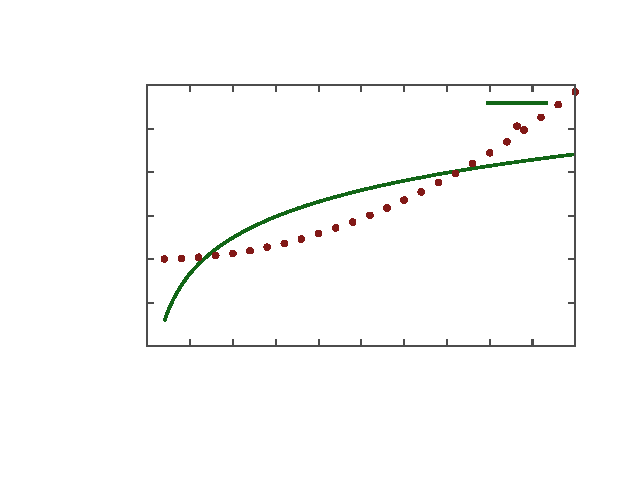
\includegraphics{./graficos/ajuste-burbuja-malo}}%
    \gplfronttext
  \end{picture}%
\endgroup

	\end{center}
\end{frame}

\begin{frame}{Hanoi con función potencial de orden 4}
	\fontsize{8pt}{7.2}\selectfont
	\begin{center}
		% GNUPLOT: LaTeX picture with Postscript
\begingroup
  \makeatletter
  \providecommand\color[2][]{%
    \GenericError{(gnuplot) \space\space\space\@spaces}{%
      Package color not loaded in conjunction with
      terminal option `colourtext'%
    }{See the gnuplot documentation for explanation.%
    }{Either use 'blacktext' in gnuplot or load the package
      color.sty in LaTeX.}%
    \renewcommand\color[2][]{}%
  }%
  \providecommand\includegraphics[2][]{%
    \GenericError{(gnuplot) \space\space\space\@spaces}{%
      Package graphicx or graphics not loaded%
    }{See the gnuplot documentation for explanation.%
    }{The gnuplot epslatex terminal needs graphicx.sty or graphics.sty.}%
    \renewcommand\includegraphics[2][]{}%
  }%
  \providecommand\rotatebox[2]{#2}%
  \@ifundefined{ifGPcolor}{%
    \newif\ifGPcolor
    \GPcolortrue
  }{}%
  \@ifundefined{ifGPblacktext}{%
    \newif\ifGPblacktext
    \GPblacktextfalse
  }{}%
  % define a \g@addto@macro without @ in the name:
  \let\gplgaddtomacro\g@addto@macro
  % define empty templates for all commands taking text:
  \gdef\gplbacktext{}%
  \gdef\gplfronttext{}%
  \makeatother
  \ifGPblacktext
    % no textcolor at all
    \def\colorrgb#1{}%
    \def\colorgray#1{}%
  \else
    % gray or color?
    \ifGPcolor
      \def\colorrgb#1{\color[rgb]{#1}}%
      \def\colorgray#1{\color[gray]{#1}}%
      \expandafter\def\csname LTw\endcsname{\color{white}}%
      \expandafter\def\csname LTb\endcsname{\color{black}}%
      \expandafter\def\csname LTa\endcsname{\color{black}}%
      \expandafter\def\csname LT0\endcsname{\color[rgb]{1,0,0}}%
      \expandafter\def\csname LT1\endcsname{\color[rgb]{0,1,0}}%
      \expandafter\def\csname LT2\endcsname{\color[rgb]{0,0,1}}%
      \expandafter\def\csname LT3\endcsname{\color[rgb]{1,0,1}}%
      \expandafter\def\csname LT4\endcsname{\color[rgb]{0,1,1}}%
      \expandafter\def\csname LT5\endcsname{\color[rgb]{1,1,0}}%
      \expandafter\def\csname LT6\endcsname{\color[rgb]{0,0,0}}%
      \expandafter\def\csname LT7\endcsname{\color[rgb]{1,0.3,0}}%
      \expandafter\def\csname LT8\endcsname{\color[rgb]{0.5,0.5,0.5}}%
    \else
      % gray
      \def\colorrgb#1{\color{black}}%
      \def\colorgray#1{\color[gray]{#1}}%
      \expandafter\def\csname LTw\endcsname{\color{white}}%
      \expandafter\def\csname LTb\endcsname{\color{black}}%
      \expandafter\def\csname LTa\endcsname{\color{black}}%
      \expandafter\def\csname LT0\endcsname{\color{black}}%
      \expandafter\def\csname LT1\endcsname{\color{black}}%
      \expandafter\def\csname LT2\endcsname{\color{black}}%
      \expandafter\def\csname LT3\endcsname{\color{black}}%
      \expandafter\def\csname LT4\endcsname{\color{black}}%
      \expandafter\def\csname LT5\endcsname{\color{black}}%
      \expandafter\def\csname LT6\endcsname{\color{black}}%
      \expandafter\def\csname LT7\endcsname{\color{black}}%
      \expandafter\def\csname LT8\endcsname{\color{black}}%
    \fi
  \fi
    \setlength{\unitlength}{0.0500bp}%
    \ifx\gptboxheight\undefined%
      \newlength{\gptboxheight}%
      \newlength{\gptboxwidth}%
      \newsavebox{\gptboxtext}%
    \fi%
    \setlength{\fboxrule}{0.5pt}%
    \setlength{\fboxsep}{1pt}%
\begin{picture}(5760.00,4320.00)%
    \gplgaddtomacro\gplbacktext{%
      \colorrgb{0.30,0.30,0.30}%
      \put(1122,873){\makebox(0,0)[r]{\strut{}$\textcolor{text}{-1}$}}%
      \colorrgb{0.30,0.30,0.30}%
      \put(1122,1221){\makebox(0,0)[r]{\strut{}$\textcolor{text}{0}$}}%
      \colorrgb{0.30,0.30,0.30}%
      \put(1122,1570){\makebox(0,0)[r]{\strut{}$\textcolor{text}{1}$}}%
      \colorrgb{0.30,0.30,0.30}%
      \put(1122,1918){\makebox(0,0)[r]{\strut{}$\textcolor{text}{2}$}}%
      \colorrgb{0.30,0.30,0.30}%
      \put(1122,2266){\makebox(0,0)[r]{\strut{}$\textcolor{text}{3}$}}%
      \colorrgb{0.30,0.30,0.30}%
      \put(1122,2614){\makebox(0,0)[r]{\strut{}$\textcolor{text}{4}$}}%
      \colorrgb{0.30,0.30,0.30}%
      \put(1122,2963){\makebox(0,0)[r]{\strut{}$\textcolor{text}{5}$}}%
      \colorrgb{0.30,0.30,0.30}%
      \put(1122,3311){\makebox(0,0)[r]{\strut{}$\textcolor{text}{6}$}}%
      \colorrgb{0.30,0.30,0.30}%
      \put(1122,3659){\makebox(0,0)[r]{\strut{}$\textcolor{text}{7}$}}%
      \colorrgb{0.30,0.30,0.30}%
      \put(1254,741){\rotatebox{45}{\makebox(0,0)[r]{\strut{}$\textcolor{text}{5}$}}}%
      \colorrgb{0.30,0.30,0.30}%
      \put(2076,741){\rotatebox{45}{\makebox(0,0)[r]{\strut{}$\textcolor{text}{10}$}}}%
      \colorrgb{0.30,0.30,0.30}%
      \put(2898,741){\rotatebox{45}{\makebox(0,0)[r]{\strut{}$\textcolor{text}{15}$}}}%
      \colorrgb{0.30,0.30,0.30}%
      \put(3719,741){\rotatebox{45}{\makebox(0,0)[r]{\strut{}$\textcolor{text}{20}$}}}%
      \colorrgb{0.30,0.30,0.30}%
      \put(4541,741){\rotatebox{45}{\makebox(0,0)[r]{\strut{}$\textcolor{text}{25}$}}}%
      \colorrgb{0.30,0.30,0.30}%
      \put(5363,741){\rotatebox{45}{\makebox(0,0)[r]{\strut{}$\textcolor{text}{30}$}}}%
    }%
    \gplgaddtomacro\gplfronttext{%
      \colorrgb{0.30,0.30,0.30}%
      \put(220,2266){\rotatebox{-270}{\makebox(0,0){\strut{}Tiempo de ejecución (s)}}}%
      \colorrgb{0.30,0.30,0.30}%
      \put(3308,220){\makebox(0,0){\strut{}Tamaño del vector (elementos)}}%
      \colorrgb{0.30,0.30,0.30}%
      \put(3308,3989){\makebox(0,0){\strut{}Ajuste Hanoi potencial de orden 4}}%
      \csname LTb\endcsname%
      \put(4376,3486){\makebox(0,0)[r]{\strut{}0.00$x^4$+-0.01$x^3$ + 0.27$x^2$ + -2.34$x$ +  6.68}}%
      \csname LTb\endcsname%
      \put(4376,3266){\makebox(0,0)[r]{\strut{}Hanoi}}%
    }%
    \gplbacktext
    \put(0,0){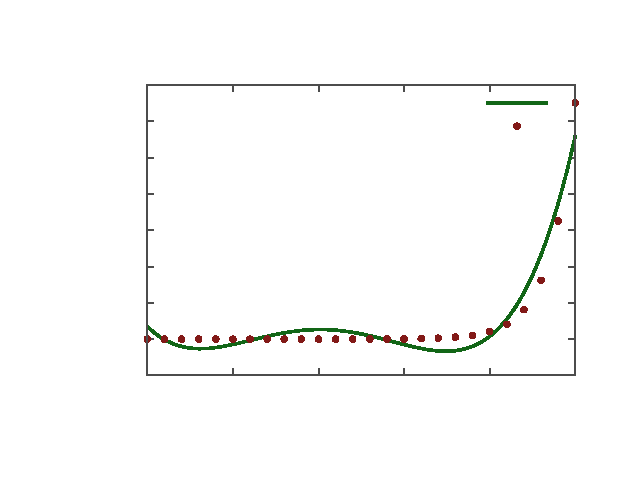
\includegraphics{./graficos/ajuste-hanoi-malo}}%
    \gplfronttext
  \end{picture}%
\endgroup

	\end{center}
\end{frame}


\begin{frame}{Características de los PC donde se ha ejecutado}
\begin{itemize}
\item Apple MacBook Pro, Intel(R) Core(TM) i5-5257U CPU @ 2.70GHz, 8GB RAM.\\  Compilador: clang-800.0.38 \\
Sistema operativo: macOS Sierra
\vskip 0.5 cm
\item Dell XPS 13, Intel(R) Core(TM) i5-7200U CPU @ 2.50GHz, 8GB RAM.\\
Compilador: g++ 6.3.1\\
Sistema operativo: Arch Linux
\end{itemize}
	
\end{frame}

\end{document}

